% compile with XeLaTeX
\documentclass[dvipsnames,mathserif]{beamer}
%\definecolor{links}{HTML}{2A1B81}
\definecolor{links}{HTML}{159fea}

\hypersetup{colorlinks,linkcolor=,urlcolor=links}
%\setbeamerfont{title}{size=\tiny}
\setbeamertemplate{footline}[frame number]
\setbeamercolor{footline}{fg=black}
\setbeamerfont{footline}{series=\bfseries}

\usepackage{tikz, babel}
\usepackage[export]{adjustbox}

\usetheme{Frankfurt}%1
%\usetheme{Darmstadt}%1

\makeatother

\setbeamerfont*{itemize/enumerate body}{size=\fontsize{9}{11}}
\setbeamerfont*{itemize/enumerate subbody}{parent=itemize/enumerate body}
\setbeamerfont*{itemize/enumerate subsubbody}{parent=itemize/enumerate body}

%% for RTL liste
%\makeatletter
%\newcommand{\RTListe}{\raggedleft\rightskip\leftm}
%\newcommand{\leftm}{\@totalleftmargin}
%\makeatother
%
%% RTL frame title
%\setbeamertemplate{frametitle}
%{\vspace*{-1mm}
%  \nointerlineskip
%    \begin{beamercolorbox}[sep=0.3cm,ht=2.2em,wd=\paperwidth]{frametitle}
%        \vbox{}\vskip-2ex%
%        \strut\hskip1ex\insertframetitle\strut
%        \vskip-0.8ex%
%    \end{beamercolorbox}
%}
%% align subsection in toc
%\makeatletter
%\setbeamertemplate{subsection in toc}
%{\leavevmode\rightskip=5ex%
%  \llap{\raise0.1ex\beamer@usesphere{subsection number projected}{bigsphere}\kern1ex}%
%  \inserttocsubsection\par%
%}
%\makeatother
%
%% RTL triangle for itemize
%\setbeamertemplate{itemize item}{\scriptsize\raise1.25pt\hbox{\donotcoloroutermaths$\blacktriangleleft$}} 
%
%%\setbeamertemplate{itemize item}{\rule{4pt}{4pt}}
%
%\defbeamertemplate{enumerate item}{square2}
%{\LR{
%    %
%    \hbox{%
%    \usebeamerfont*{item projected}%
%    \usebeamercolor[bg]{item projected}%
%    \vrule width2.25ex height1.85ex depth.4ex%
%    \hskip-2.25ex%
%    \hbox to2.25ex{%
%      \hfil%
%      {\color{fg}\insertenumlabel}%
%      \hfil}%
%  }%
%}}
%
%\setbeamertemplate{enumerate item}[square2]

%\setbeamertemplate{footline}{} %gets rid of footer completely
\setbeamertemplate{navigation symbols}{}


\titlegraphic { 
\begin{tikzpicture}[overlay,remember picture, opacity=0.1,]
\node[] at (0, 2.9){
    
\includegraphics[width=0.63\textwidth]{iCapital_logo_RGB.png}
};\end{tikzpicture}}
\setbeamertemplate{caption}[numbered]
\begin{document}

\rightskip\rightmargin
\title{Kalman Filters 101}
\author{ \Large \textbf{} }
\institute{\large\textbf{}\\
Arnav Sheth \\
iCapital Network}
\footnotesize{\date{January 17, 2023 }


\begin{frame}
	\maketitle
\end{frame}

\begin{frame}{Summary}
	\footnotesize \tableofcontents
\end{frame}

\section{Intro}

\begin{frame}{What is a Kalman Filter?}
    \begin{itemize}
    	\item State space model or regime-switching model.
	\item Traditionally rooted in engineering applications.
	\begin{itemize}
		\item For example, autonomous vehicles or trajectory analysis.
	\end{itemize}
	\item Now used in economics/finance.
	\item Can be interpreted as a natural extension of traditional ARMA models\footnote{\tiny See Harvey (1989), for example.}.
	\begin{itemize}
		\item Makes it easier to explain.
	\end{itemize}
    \end{itemize}
\end{frame}


\begin{frame}{What is a Kalman Filter?}
	\begin{itemize}
		\item Introduced in 1960 by Rudolf Kalman and Ruslan Bucy\footnote{\tiny See Kalman (1960) and Kalman and Bucy (1961).}. 
%		\begin{itemize}
%			\item Concept of state variables and state space of dynamical systems.
%		\end{itemize}
		\begin{block}{}
			The Kalman filter is an estimator of the conditional moments of a Gaussian linear system. It is an optimal recursive algorithm.
		\end{block}
		\item Used for:
		\begin{itemize}
			\item the calibration of time series model predictor variables; 
			\item also for data smoothing applications. 
			\item Appropriate for dealing with multivariable time-varying systems and non-stationary stochastic processes.
			\begin{itemize}
				\item Is an advantage over VAR since factors are non-stationary. 
				\item It's also a more realistic assumption.
			\end{itemize}
		\end{itemize}
	\end{itemize}
\end{frame}


\begin{frame}{Why Use Kalman Filters?}
	\begin{itemize}
		\item Kalman Filters have several desirable properties:
		\begin{enumerate}
			\item They are fast; amenable to large datasets.
			\item Good at dealing with unknown structural breaks and regime changes\footnote{\tiny See Renzi-Ricci (2016).}. 
			\item They preserve OLS property of being consistent, unbiased, and efficient.
			\item Can handle missing data in a fairly straightforward manner\footnote{\tiny See Brockwell and Davis (1991).}.
			\item Because they are constructed as recursions, can handle out-of-sample forecasting well.
		\end{enumerate}
	\end{itemize}
\end{frame}

\section{The Math}

\begin{frame}{A Simple Model}
	\begin{itemize}
		\item In its simplest setup, we have\footnote{\tiny These are variables but you can replace them with $K \times 1$ vectors (say).}:
		\begin{align}
			y_t 		&= \mu_t + u_t	\label{eq:measurement} \\ 
			\mu_{t+1}	&= T_t \mu_t + \eta_t \label{eq:transition}
		\end{align}
		\begin{itemize}
			\item Equation \eqref{eq:measurement} is known as the \textit{measurement} equation. 
			\item Equation \eqref{eq:transition} is known as the \textit{transition} equation.
		\end{itemize}
		\item For even more simplicity, let's assume $T_t$ to be constant, or 1.		
		\begin{itemize}
			\item Then $\mu_t$ follows a random walk.
		\end{itemize}
	\end{itemize}
\end{frame}

\begin{frame}{A Simple Model}
	\begin{itemize}
		\item In its simplest setup, we have\footnote{\tiny These are variables but you can replace them with $K \times 1$ vectors (say).}:
		\begin{align}
			y_t 		&= \mu_t + u_t	\label{eq:measurement} \\ 
			\mu_{t+1}	&= T_t \mu_t + \eta_t \label{eq:transition}
		\end{align}
		\begin{itemize}
			\item $u_t$ and $\eta_t$ are called, respectively, \textit{measurement} and \textit{observation} noise.
			\item $u_t \sim N(0, \sigma_u^2)$, $\eta \sim N(0, \sigma_\eta^2$, and $E[u_t \eta_t] = 0$.
		\end{itemize}
		\item The latent state, $\mu_t$ is hidden (unobserved). E.g., the true beta of a company, or state of the economy. 
		\begin{itemize}
			\item The data gives us $y_t$. 
		\end{itemize}
		\pause
		\item To evaluate the size of $\sigma_\eta^2$, we use the ratio of variances: $\sigma_\eta^2 / \sigma_u^2$.
	\end{itemize}
\end{frame}

\begin{frame}{A More Complex Model}
	\begin{align}
		y_t		&=	\alpha + \beta_t x_t + u_t	\\
		\beta_{t+1} 	&=	\beta_t + \eta_t
	\end{align}
	\begin{itemize}
		\item $\beta_t$ is the hidden state variable here. 
		\item For example:
		\begin{itemize}
			\item $y_t$ could be the excess return on a stock.
			\item $x_t$ could be the excess return on a market proxy.
		\end{itemize}
		\item We could generalize further and allow Jensen's alpha to vary over time.
		\pause
		\begin{itemize}
			\item Note that this is what we called $\mu_t$ in the previous example.
		\end{itemize}
	\end{itemize}
\end{frame}

\begin{frame}{Parameter Estimation}
	\begin{itemize}
		\item In traditional MLE, parameters are the slope and intercept.
		\begin{itemize}
			\item Recall that these could be time-varying in state space models.
		\end{itemize}
		\item In this setup, $\alpha$, $\beta$, and the variances ($\sigma_\eta^2$ and $\sigma_u^2$), are all parameters.
		\item For a \textit{filter}, you plug in variance values and estimate the slope and intercept.
		\item For a \textit{smoother}, you go back and use MLE to find the values that minimize the variances.
	\end{itemize}
\end{frame}

\begin{frame}{General Steps}
	\begin{enumerate}
		\item Specify an initial value for $\beta$, $\beta_1$. 
		\item Beginning with $t = 2$, apply the Kalman filter to $\beta_t$ to provide an estimate for $\beta_{t+1}$. 
		\begin{itemize}
			\item Estimates are denoted with hats: $\widehat{\beta}_{t+1}$ and $\widehat{y}_{t+1}$.
			\item At $t+1$ compare with the actual value, and compute the prediction error, termed the \textit{Kalman gain}.
			\item Adjust $\hat{\beta}_{t+1}$ appropriately.
		\end{itemize}
		\item Use the adjusted estimate of $\beta_{t+1}$ to get an estimate for $\beta_{t+2}$.
		\item Rinse and repeat.
	\end{enumerate}
\end{frame}

\section{References}

\begin{frame}{References}
	\begin{enumerate}
	\tiny
		\item Brockwell, P. J., \& Davis, R. A. (1991). \textit{Time series: theory and methods}. Springer Science \& Business Media.
		\item Brooks, C. (2009). \textit{Introductory Econometrics for Finance}. Cambridge University Press.
		\item Harvey, A. C. (1990). \textit{Forecasting, structural time series models and the Kalman filter}. Cambridge University Press.
		\item Jalles, J. T. (2009). Structural time series models and the Kalman filter: a concise review, \href{https://papers.ssrn.com/sol3/papers.cfm?abstract_id=1496864}{SSRN}.
		\item Kalman, R. E. (1960). A new approach to linear filtering and prediction problems, \textit{Transactions of the ASME - Journal of Basic Engineering}, 83 (Series D): 95-108. 
		\item Kalman, R. E., \& Bucy, R. S. (1961). New results in linear filtering and prediction theory, \textit{Transactions of the ASME - Journal of Basic Engineering}, 82 (Series D): 35-45. 
		\item Ljungqvist, L., \& Sargent, T. J. (2018). \textit{Recursive macroeconomic theory}. MIT press.
		\item Renzi-Ricci, G. (2016). Estimating equity betas: What can a time-varying approach add. A comparison of ordinary least squares and the Kalman filter. \textit{Insights in Economics}, 1-9.
	\end{enumerate}
\end{frame}

%\section{Motivation}
%
%\setbeamertemplate{caption}{\raggedright\insertcaption\par}
%\begin{frame}{Motivation}{Notation}
%%    \begin{figure}[!ht]
%%    	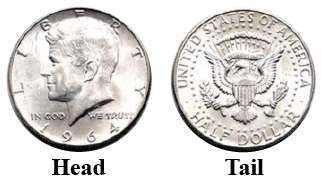
\includegraphics[width=155pt]{CoinToss2.png}
%%	\parbox{155pt}{\caption{\footnotesize  Probability and Statistics are two sides of the same coin}}
%%    \end{figure}
%
%\begin{itemize}
%	\item Let $X_{1:n} = (X_1, \ldots , X_n)$ be the outcomes of $n$ i.i.d. coin flips.
%	\item Let $\mathbb{P} (H) = \theta$, since we don't know what it is.
%	\item Probability: $\theta \longrightarrow X_{1:n}$.
%	\item Statistics: $X_{1:n} \longrightarrow \theta$.
%	\begin{itemize}
%		\item \footnotesize Maybe toss the coin a lot and look at the proportion of heads?
%	\end{itemize}
%\end{itemize}
%\end{frame}
%
%\section{Some History}
%
%\setbeamertemplate{caption}{\raggedright\insertcaption\par}
%\begin{frame}{Some History}
%%    \begin{figure}[!ht]
%%    	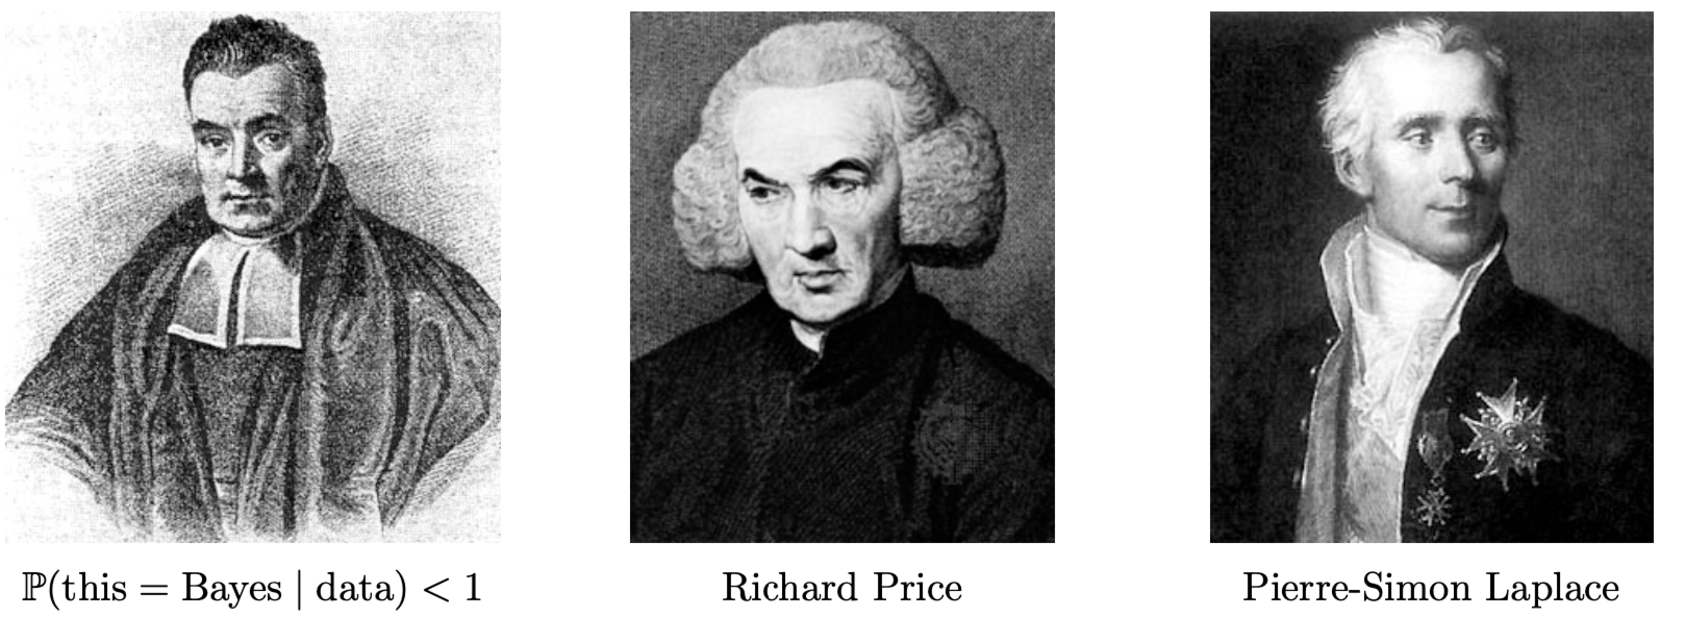
\includegraphics[width=275pt]{Bayes_etal.pdf}
%%%	\caption{$\mathcal{P}$ ( this = Bayes $\mid$ data ) $<$ 1}
%%    \end{figure}
%
%\begin{itemize}
%	\item Thomas Bayes (1701? - 1761) was a Presbyterian minister.
%	\item Work discovered by Richard Price, published in 1764.
%	\item Laplace developed it further; published in 1774.
%\end{itemize}
%
%\end{frame}
%
%
%\section{Frequentist Statistics}
%
%\begin{frame}{Frequentist Statistics}
%    \begin{itemize}
%    	\item The basic idea of frequentist statistics is that the world is described by parameters that are:
%    	\begin{itemize}
%        		\item fixed; and
%    		\item unknown.
%    	\end{itemize}
%    	\item That $\exists$ some true parameter value; we are estimating it using the sample we have.
%    	\item This true, fixed, unknown parameter describes something about the entire population.
%    \end{itemize}
%\end{frame}
%
%\section{Bayesian Statistics}
%
%
%\begin{frame}{Bayesian Statistics}
%    \begin{itemize}
%    	\item Bayesian statistics applies probabilistic methods and reasoning directly to the \textit{parameters}.
%    	\item Use the algebra of probabilities to quantify and describe how much we believe various propositions.
%	\item Bayesians apply probabilities directly to their knowledge of the world.
%	\begin{itemize}
%		\item \footnotesize Frequentists can only apply probabilities to the act of repeating an experiment.
%	\end{itemize}
%    \end{itemize}	
%\end{frame}
%
%\begin{frame}{The Math}
%	\begin{itemize}
%		\item Basic idea: assume a \textbf{prior} probability distribution for $\theta$.
%		\begin{itemize}
%			\item \footnotesize This represents the \textit{plausibility} of each possible value of $\theta$, BEFORE the data is observed.
%		\end{itemize}
%		\item The \textbf{posterior} distribution is used to make inferences about $\theta$.
%		\begin{itemize}
%			\item \footnotesize This represents the \textit{plausibility} of each possible value of $\theta$, AFTER the data is observed.
%		\end{itemize}
%		\item Mathematically, this is expressed:
%		\begin{align*}
%			p(\theta \mid x) = \frac{p(x \mid \theta) \times p(\theta)}{p(x)} 	&\propto p(x \mid \theta) \times p(\theta)	\\
%			\text{posterior~} \hspace{67pt} 							&\propto \text{~likelihood} \times \text{prior}
%		\end{align*}
%		where: 
%		\begin{itemize} \footnotesize
%			\item $x = x_{1:n}$ (for example, the coin flips from earlier); 
%			\item $p( \theta \mid x)$ is the posterior; 
%			\item $p(x \mid \theta)$ is the likelihood; and 
%			\item $p(\theta)$ is the prior.
%		\end{itemize}
%	\end{itemize}
%\end{frame}
%
%\section{Advantage: Bayesians?}
%
%\begin{frame}{Advantage: Bayesians?}
%%    \begin{figure}[!ht]
%%    	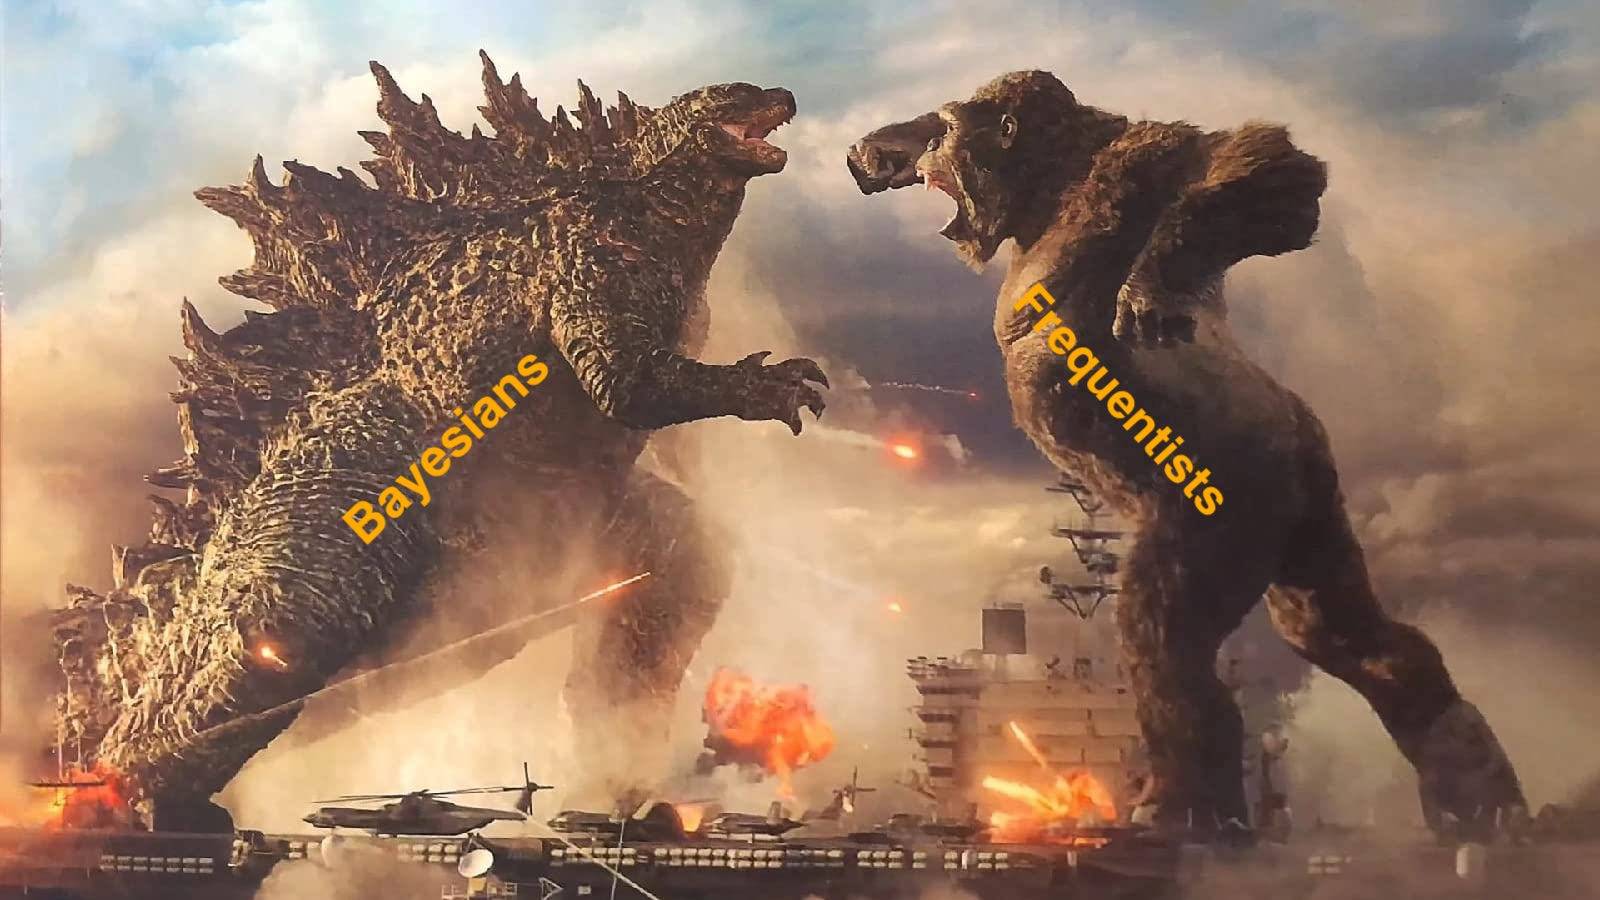
\includegraphics[height=125pt]{Godzilla_v_Kong.jpg}
%%%    	\caption{\footnotesize It's a war, baby! \text{\tiny (Just kidding)}}
%%    \end{figure}
%    
%    \begin{itemize}
%    	\item The results are understandable. \pause
%    %	\item Bayesian inference explicitly tracks and incorporates prior knowledge. \pause
%    	\item All parts of the model, including priors and other assumptions, are explicit and open to criticism. \pause
%    	\item The model is scrutable. \pause
%    	\item Admissibility. {\tiny (Thanks, Clinton)}\\
%    	{\tiny See, for example: Robert, Christian P. (1994). \textit{The Bayesian Choice}. Springer-Verlag. Also, Wald (1939).}
%    \end{itemize}
%\end{frame}
%
%\section{Some Examples}
%
%%\subsection{More Coin Tosses}
%%
%%\begin{frame}{Ten Coin Tosses}
%%    	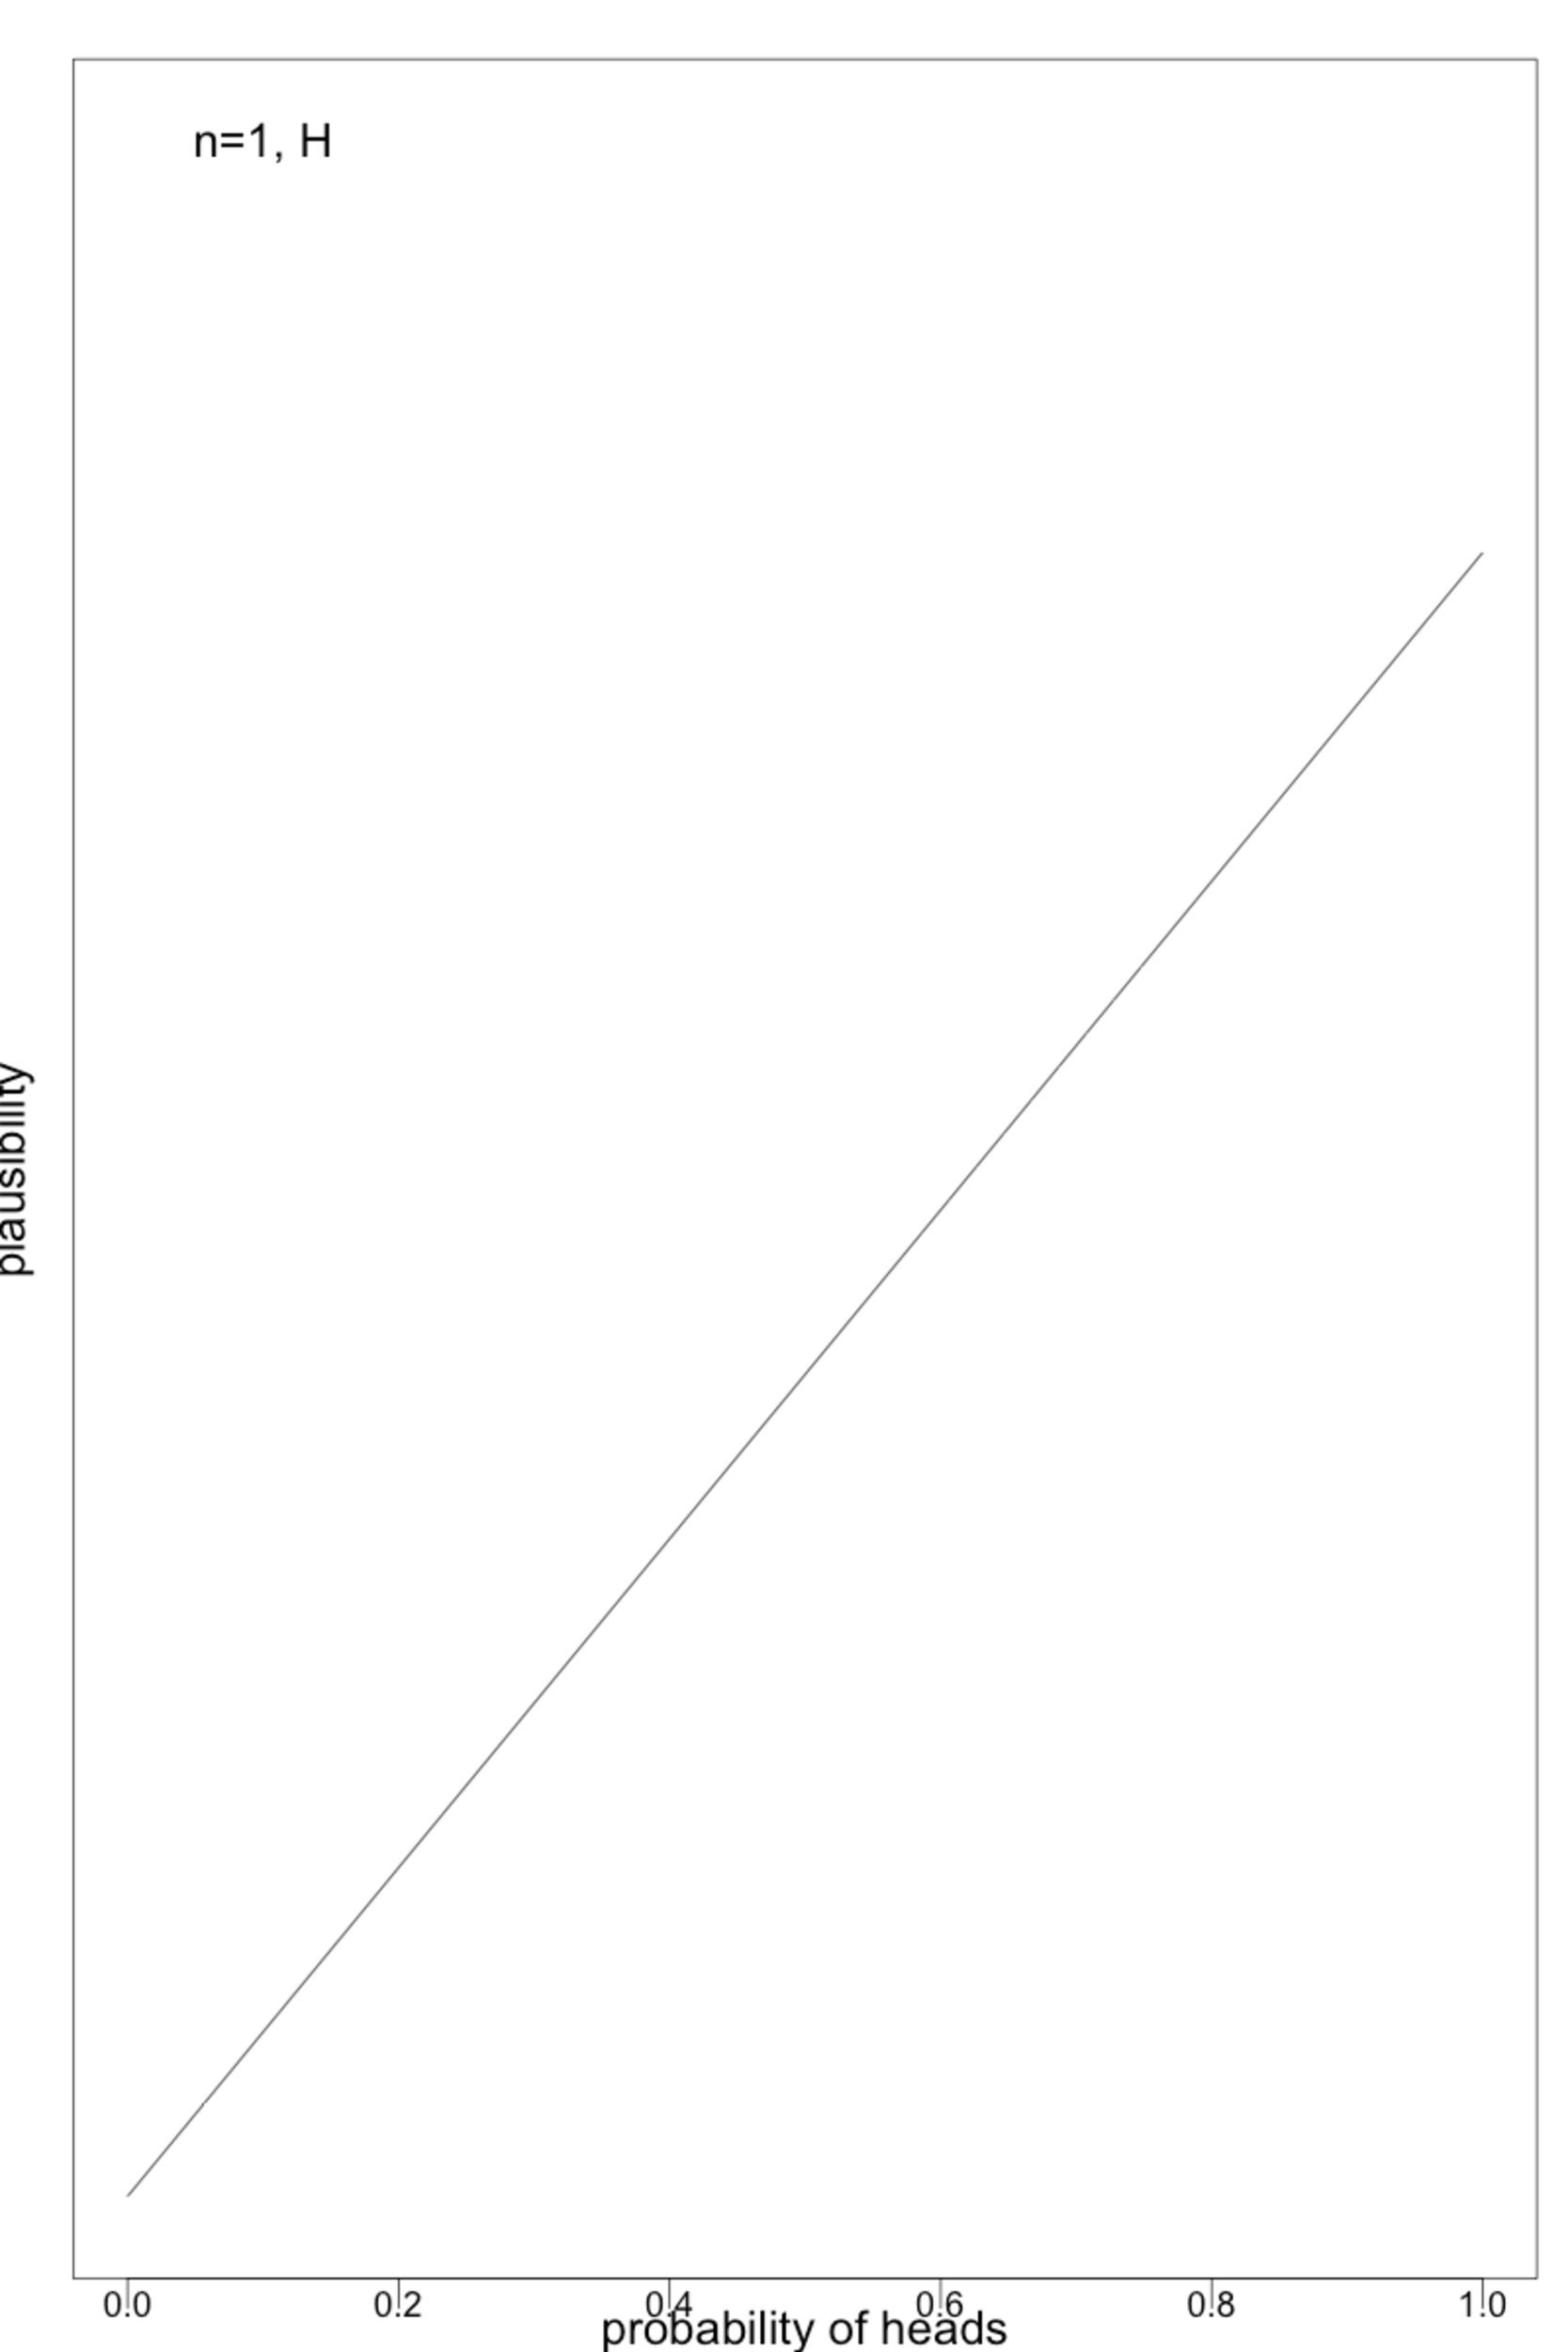
\includegraphics[width=100pt]{cointosses/One.pdf} 	\pause
%%    	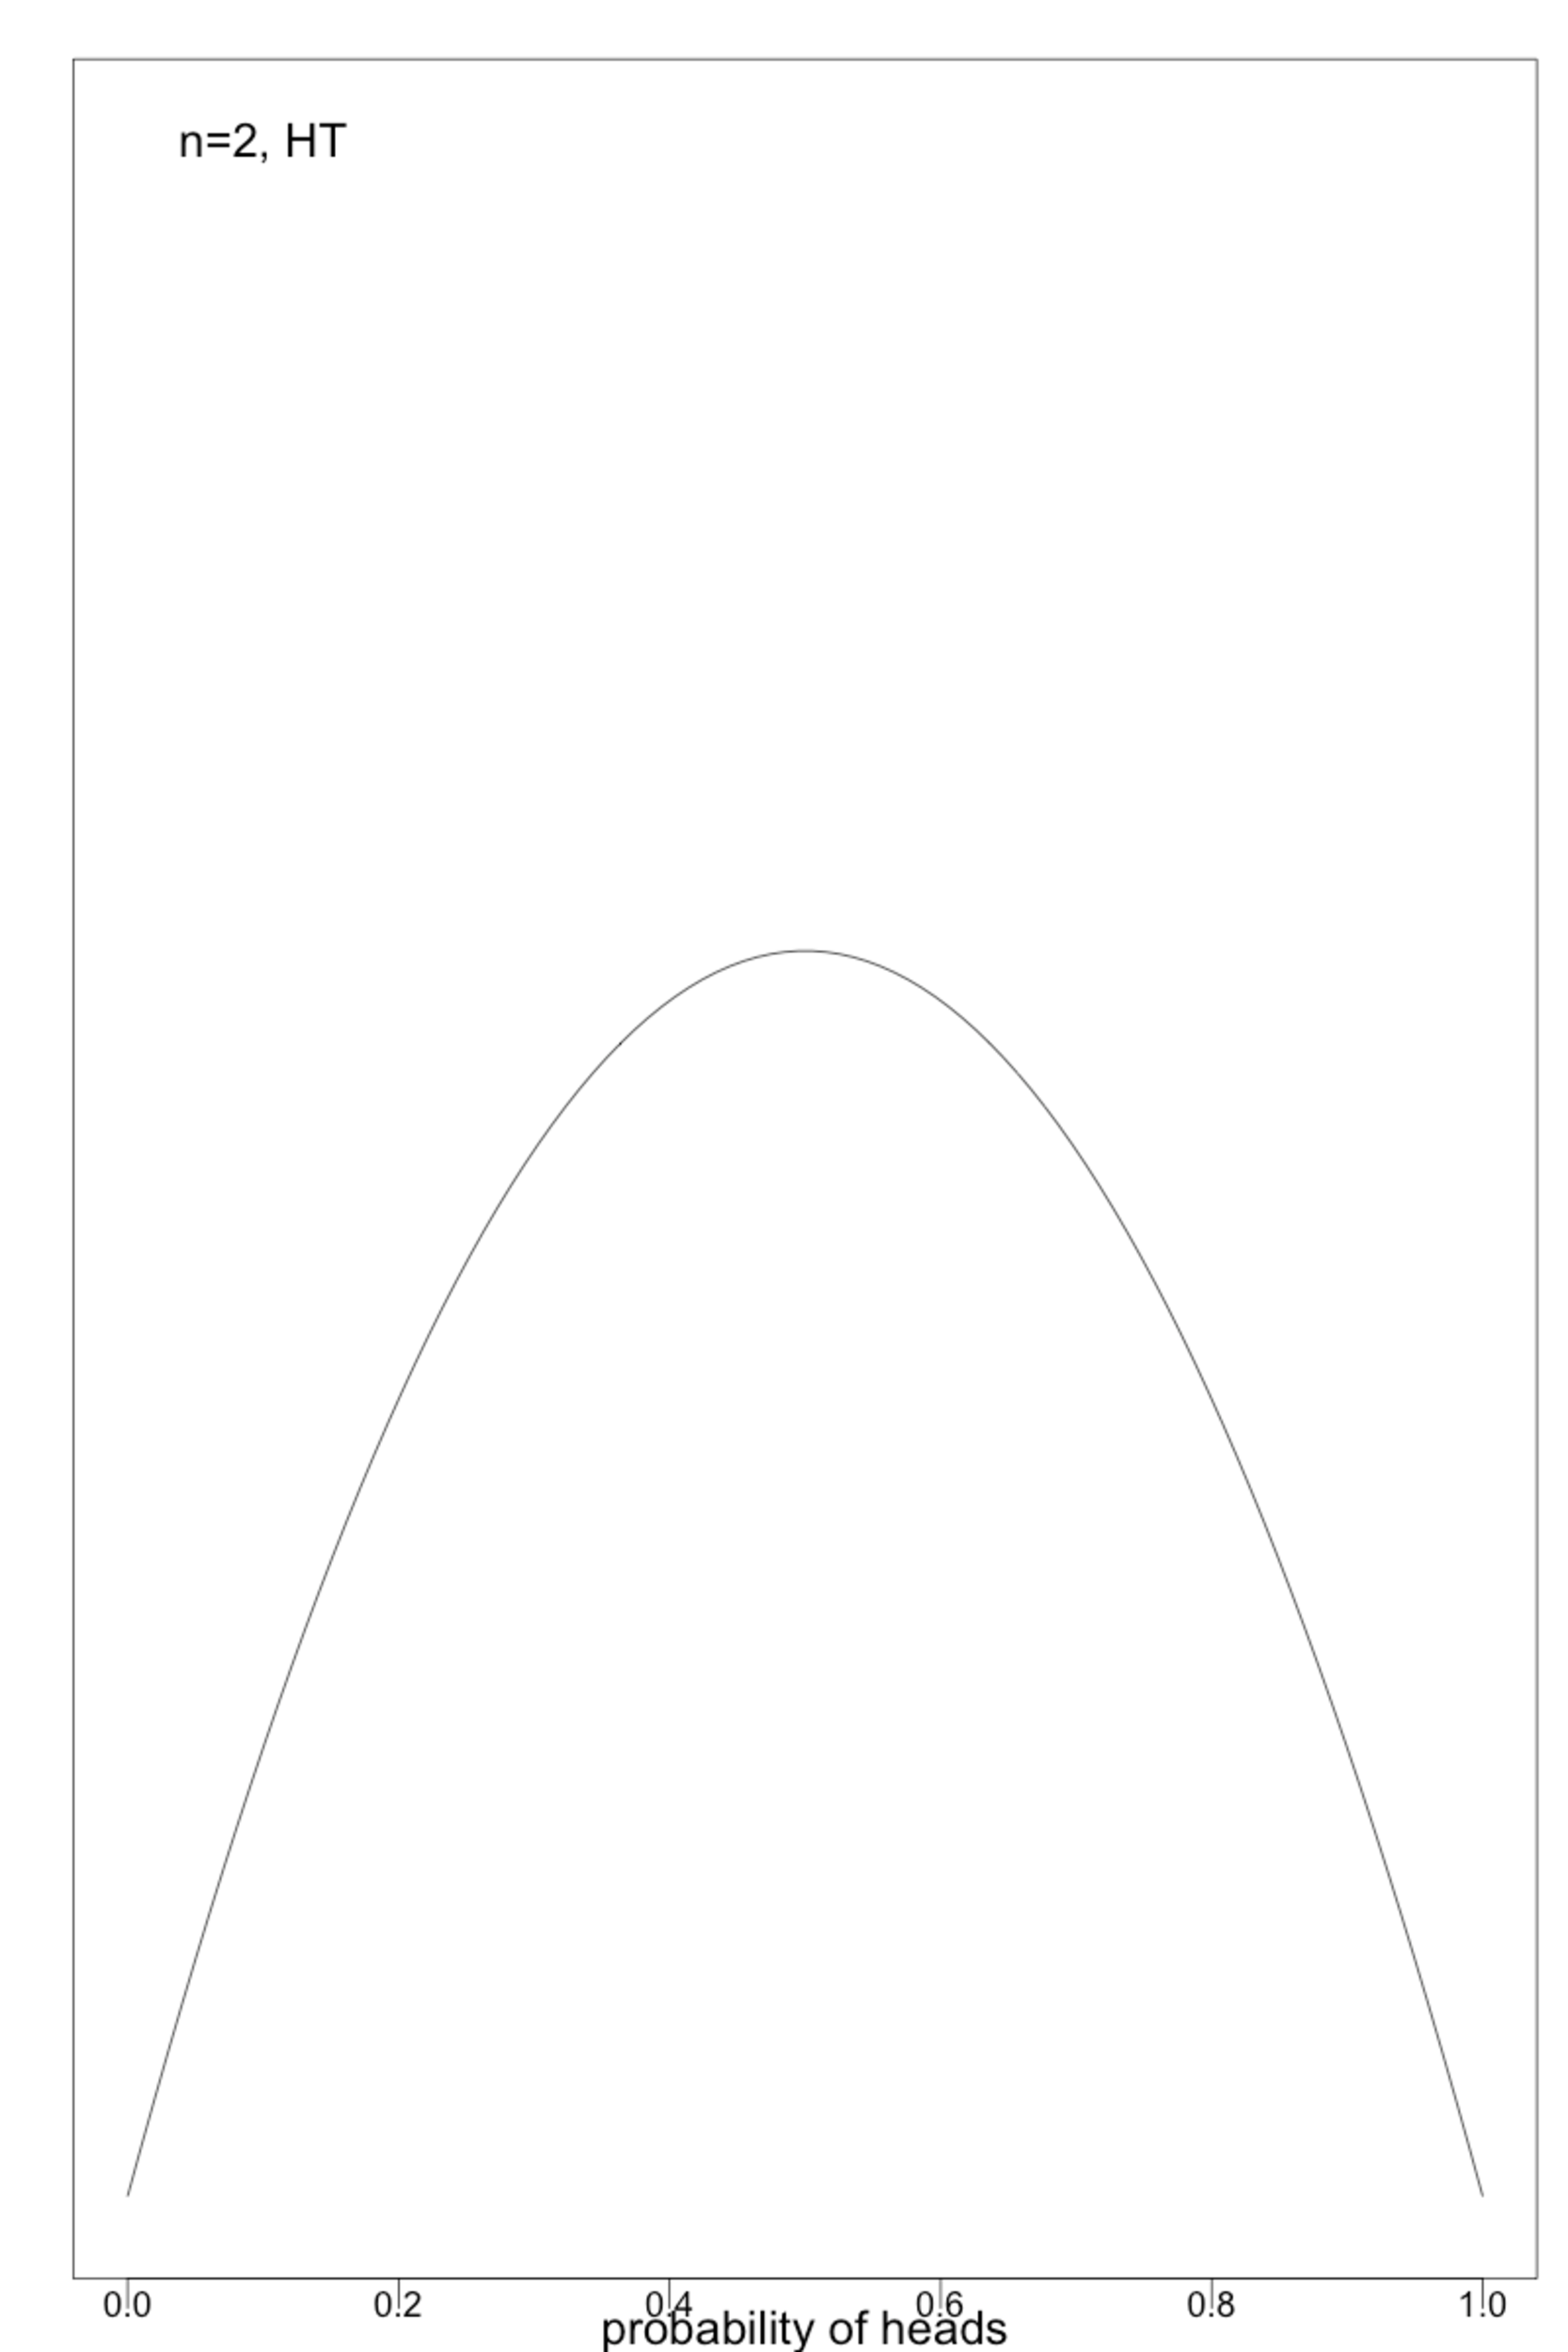
\includegraphics[width=100pt]{cointosses/Two.pdf}  	\pause
%%    	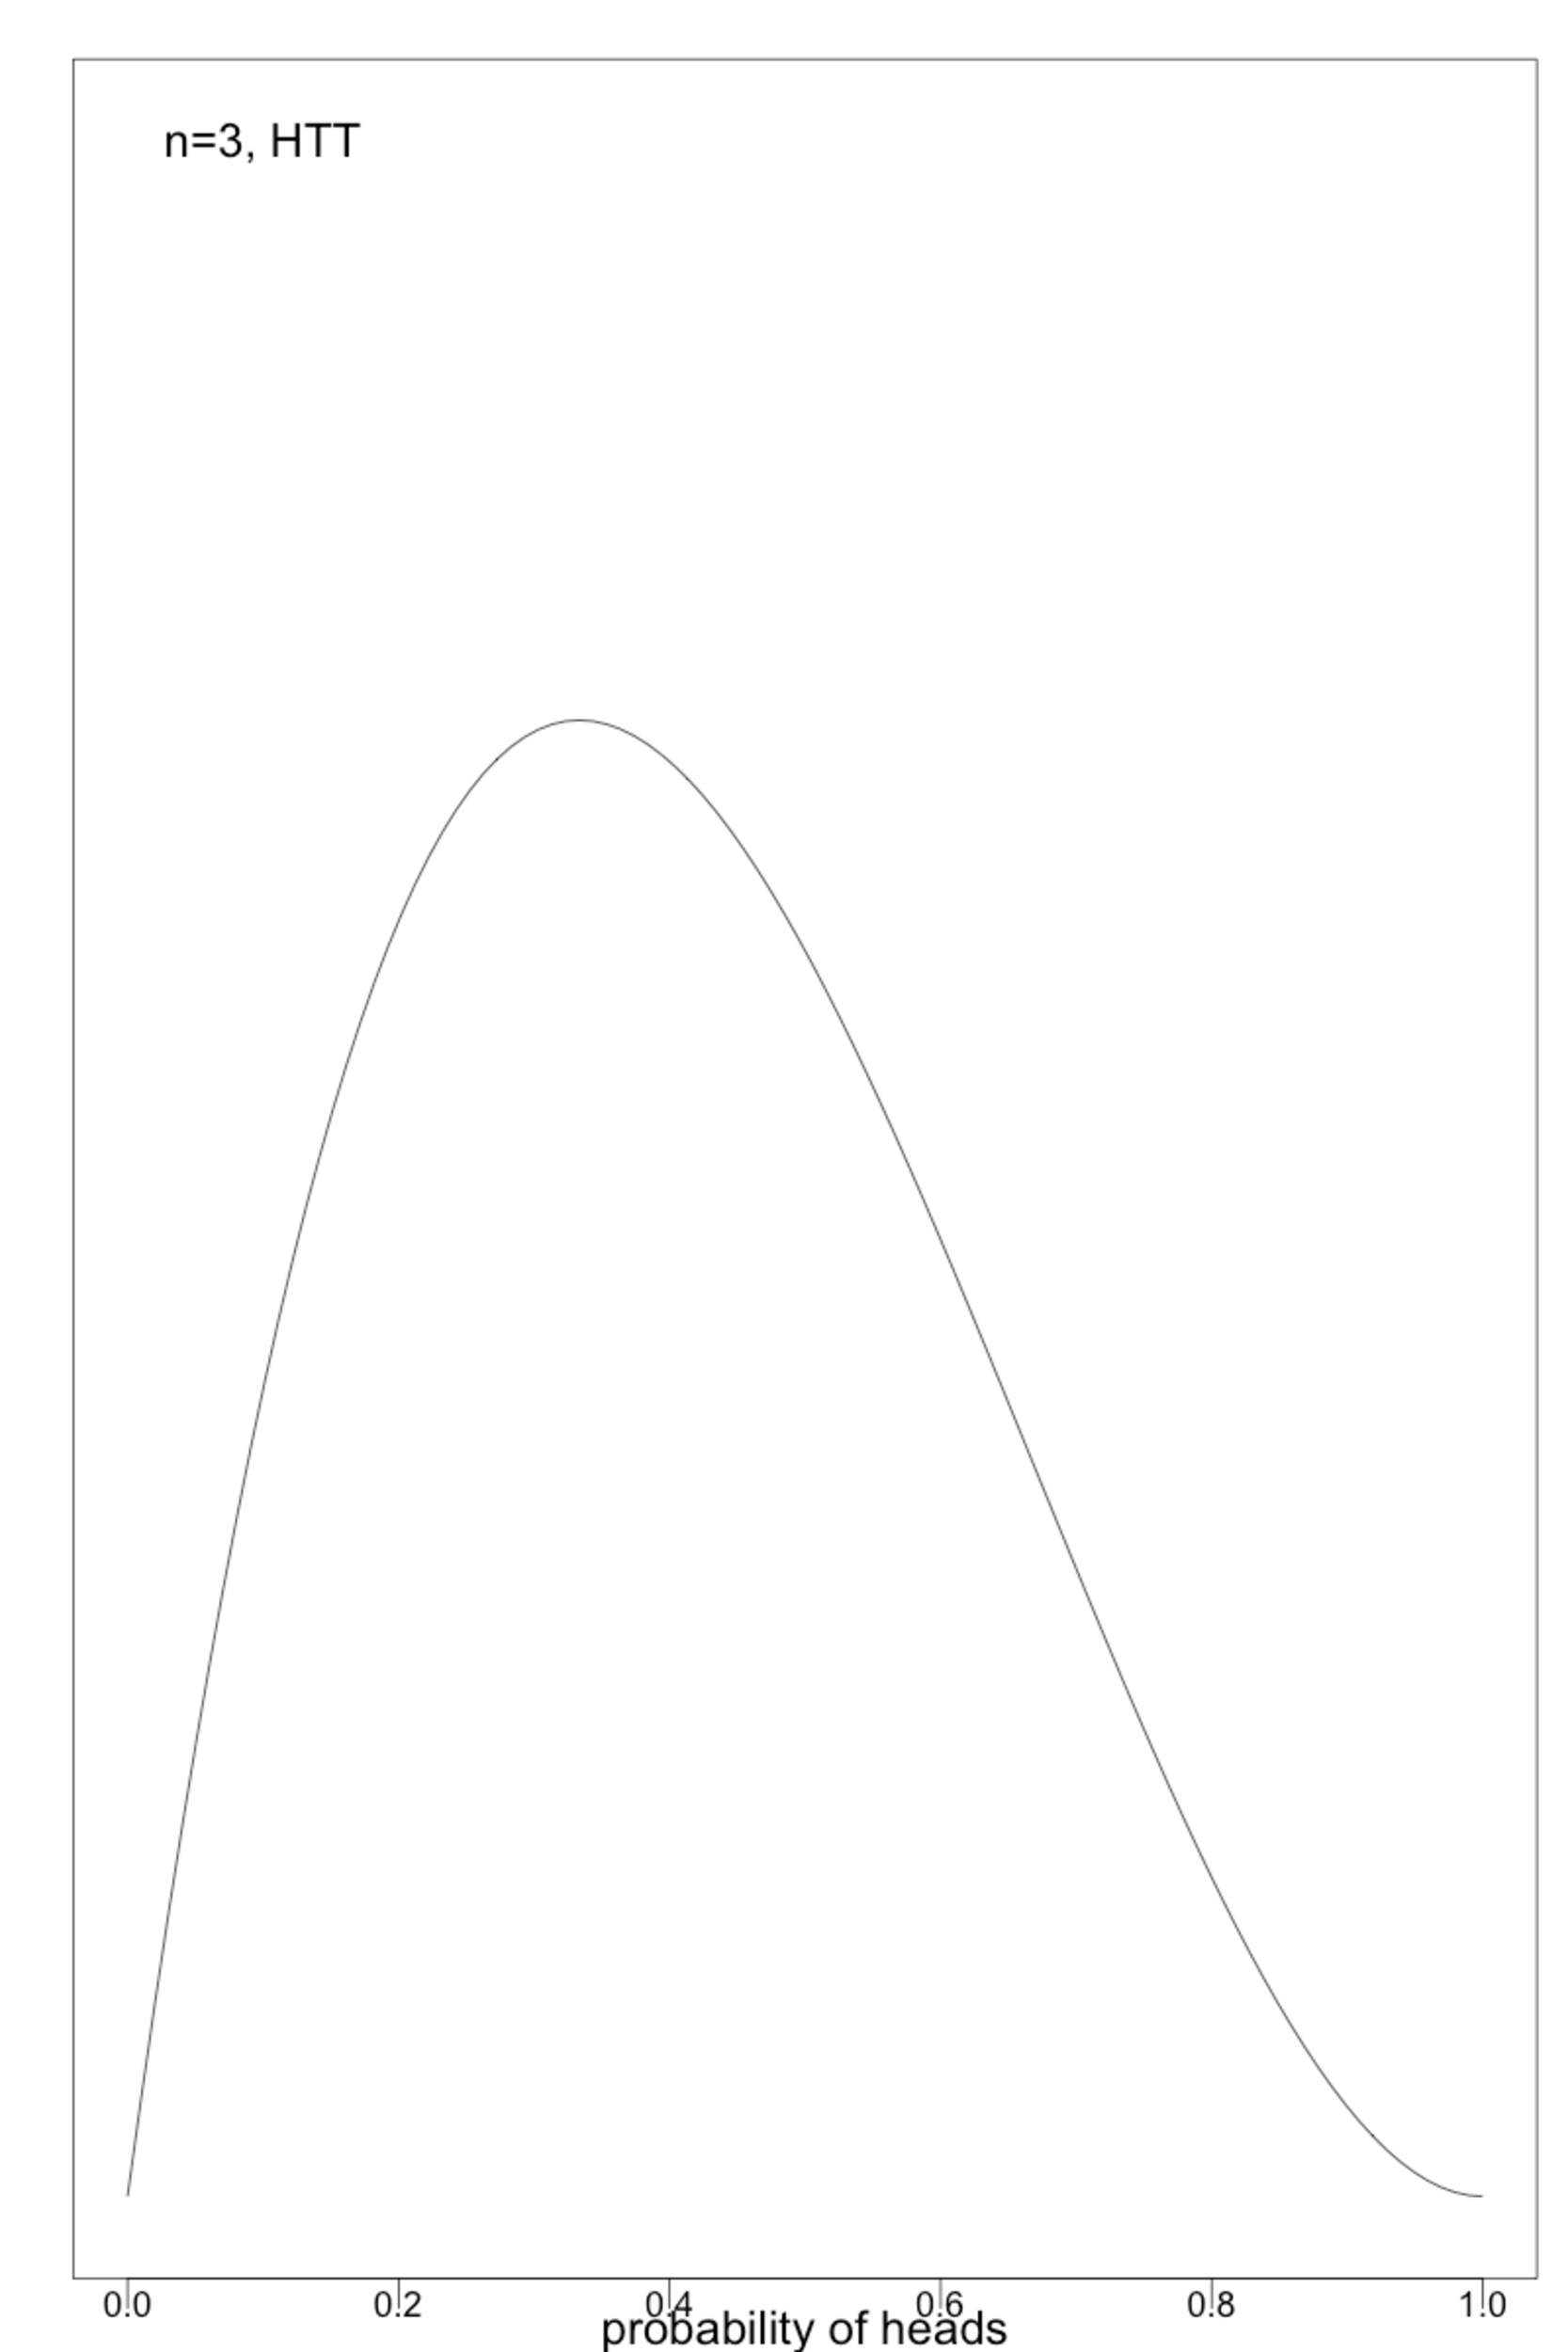
\includegraphics[width=100pt]{cointosses/Three.pdf}	
%%\end{frame}
%%
%%\begin{frame}{Ten Coin Tosses}
%%    	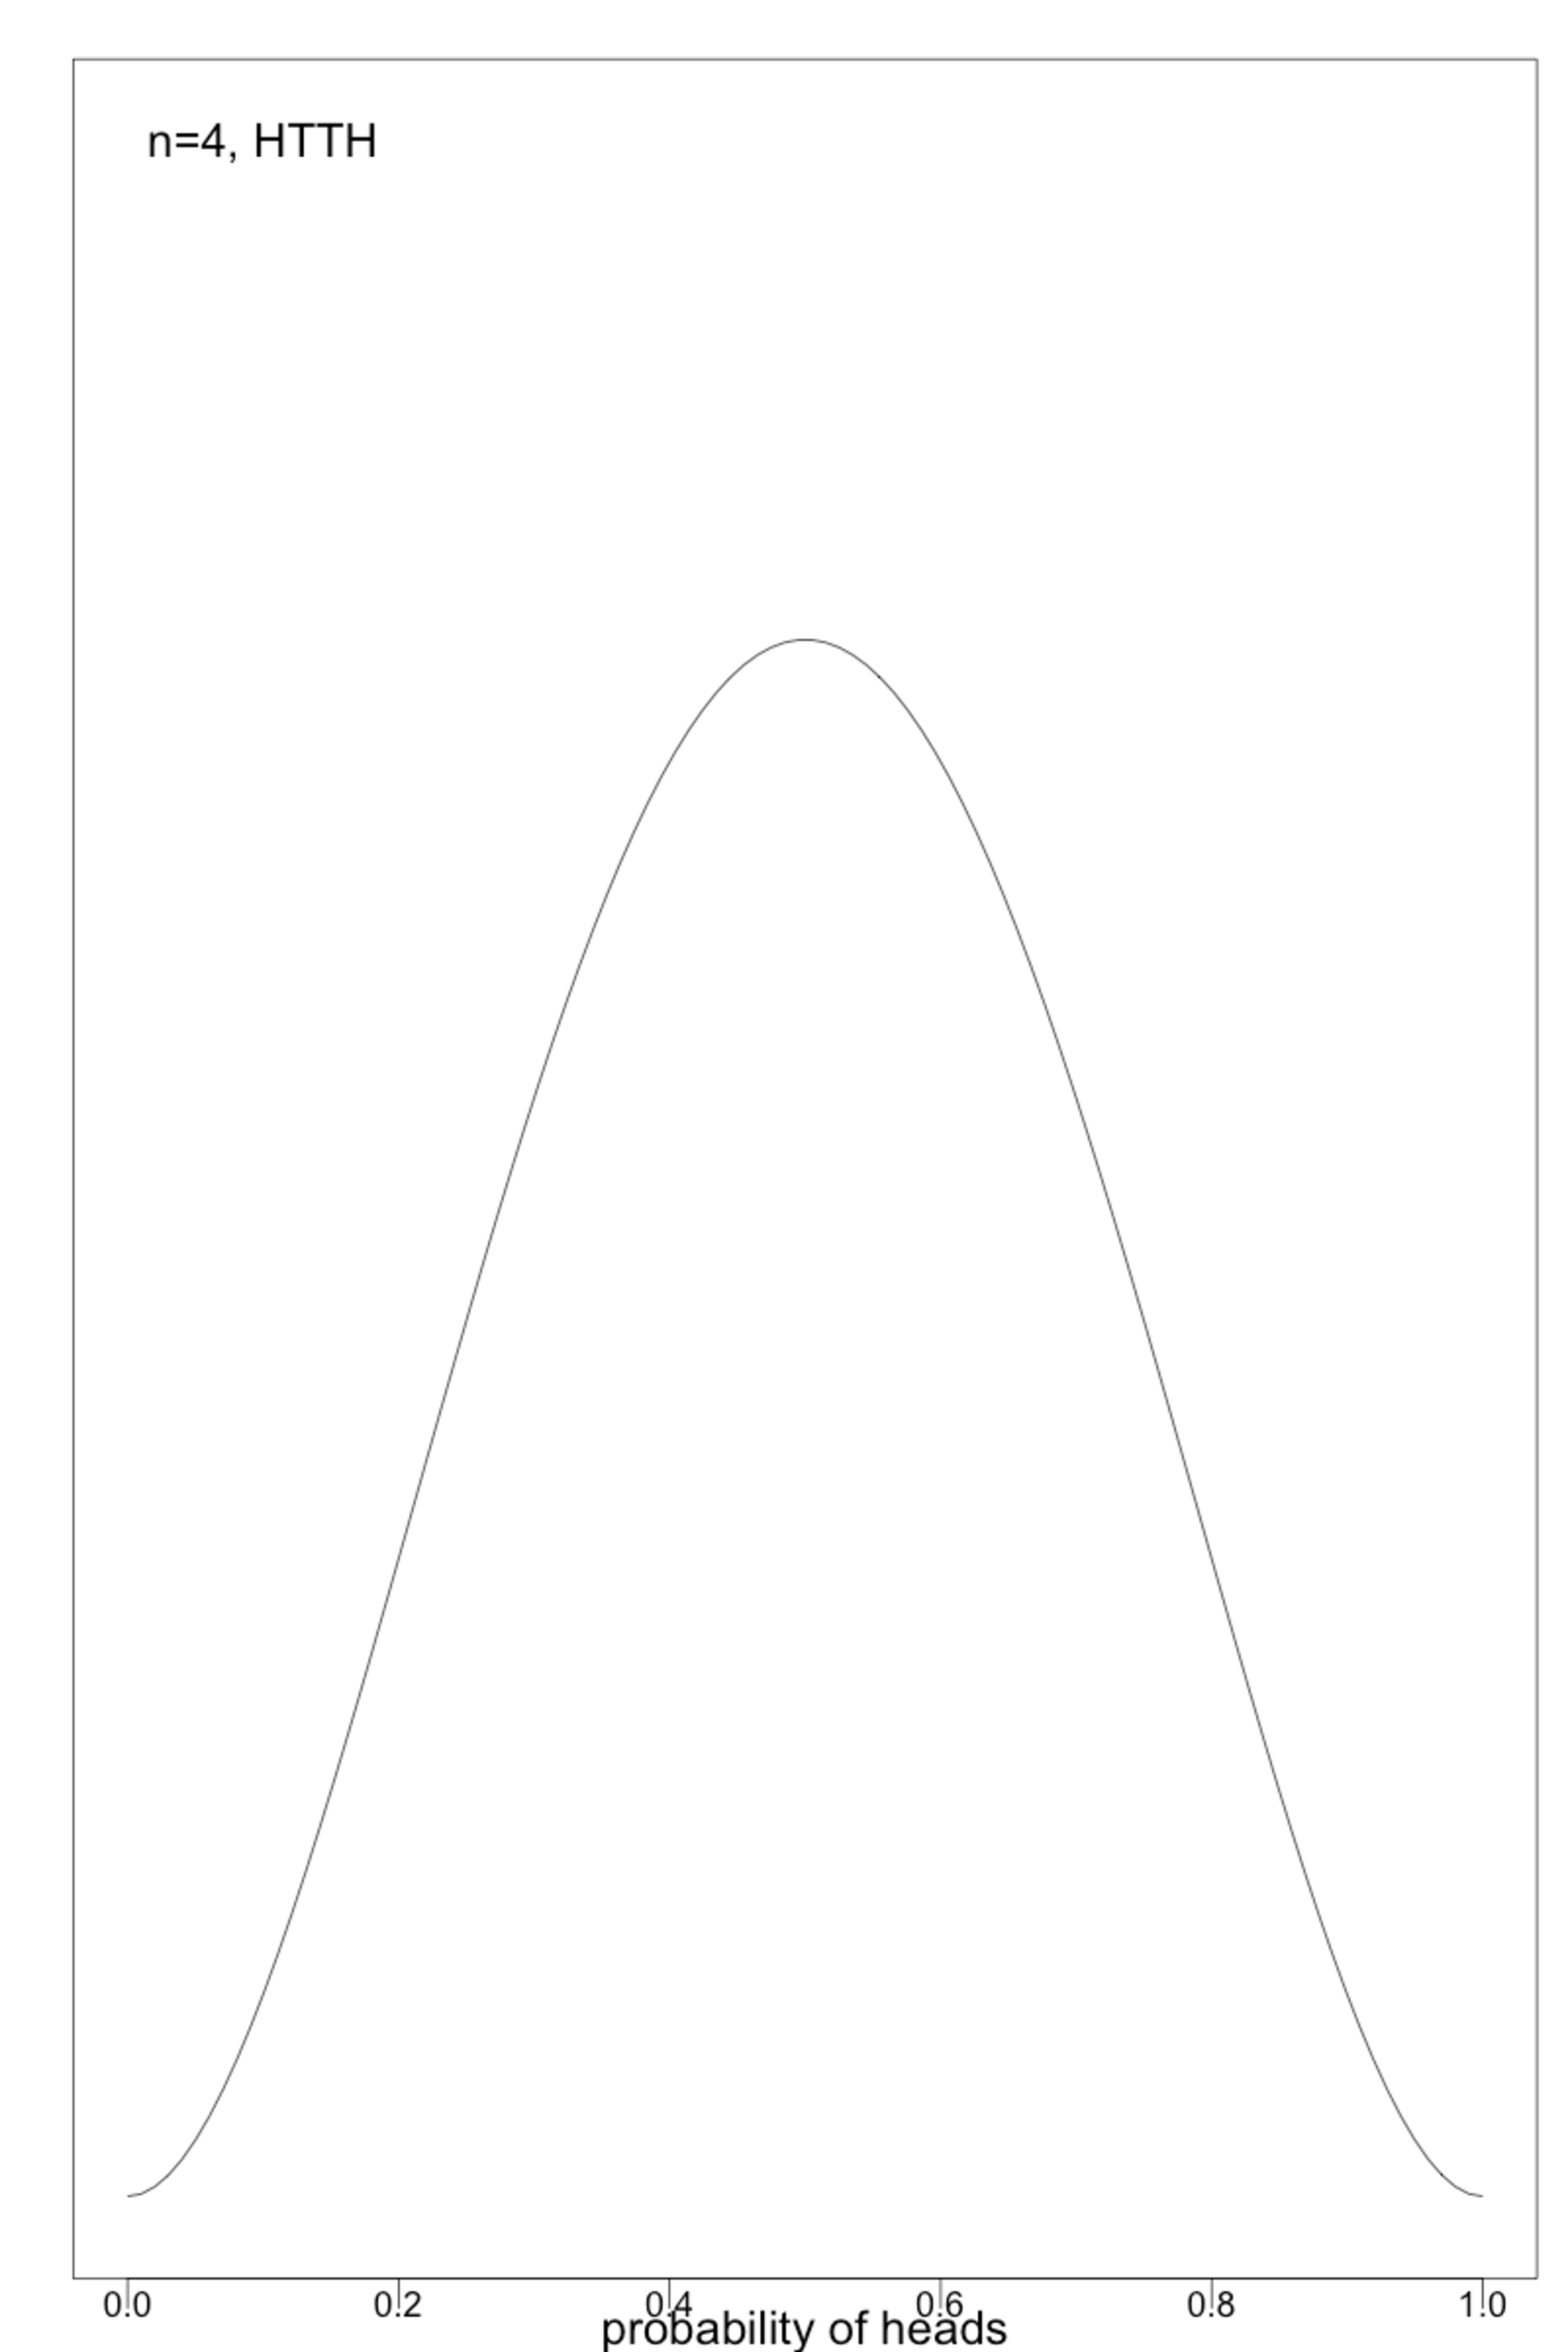
\includegraphics[width=100pt]{cointosses/Four.pdf}	\pause
%%    	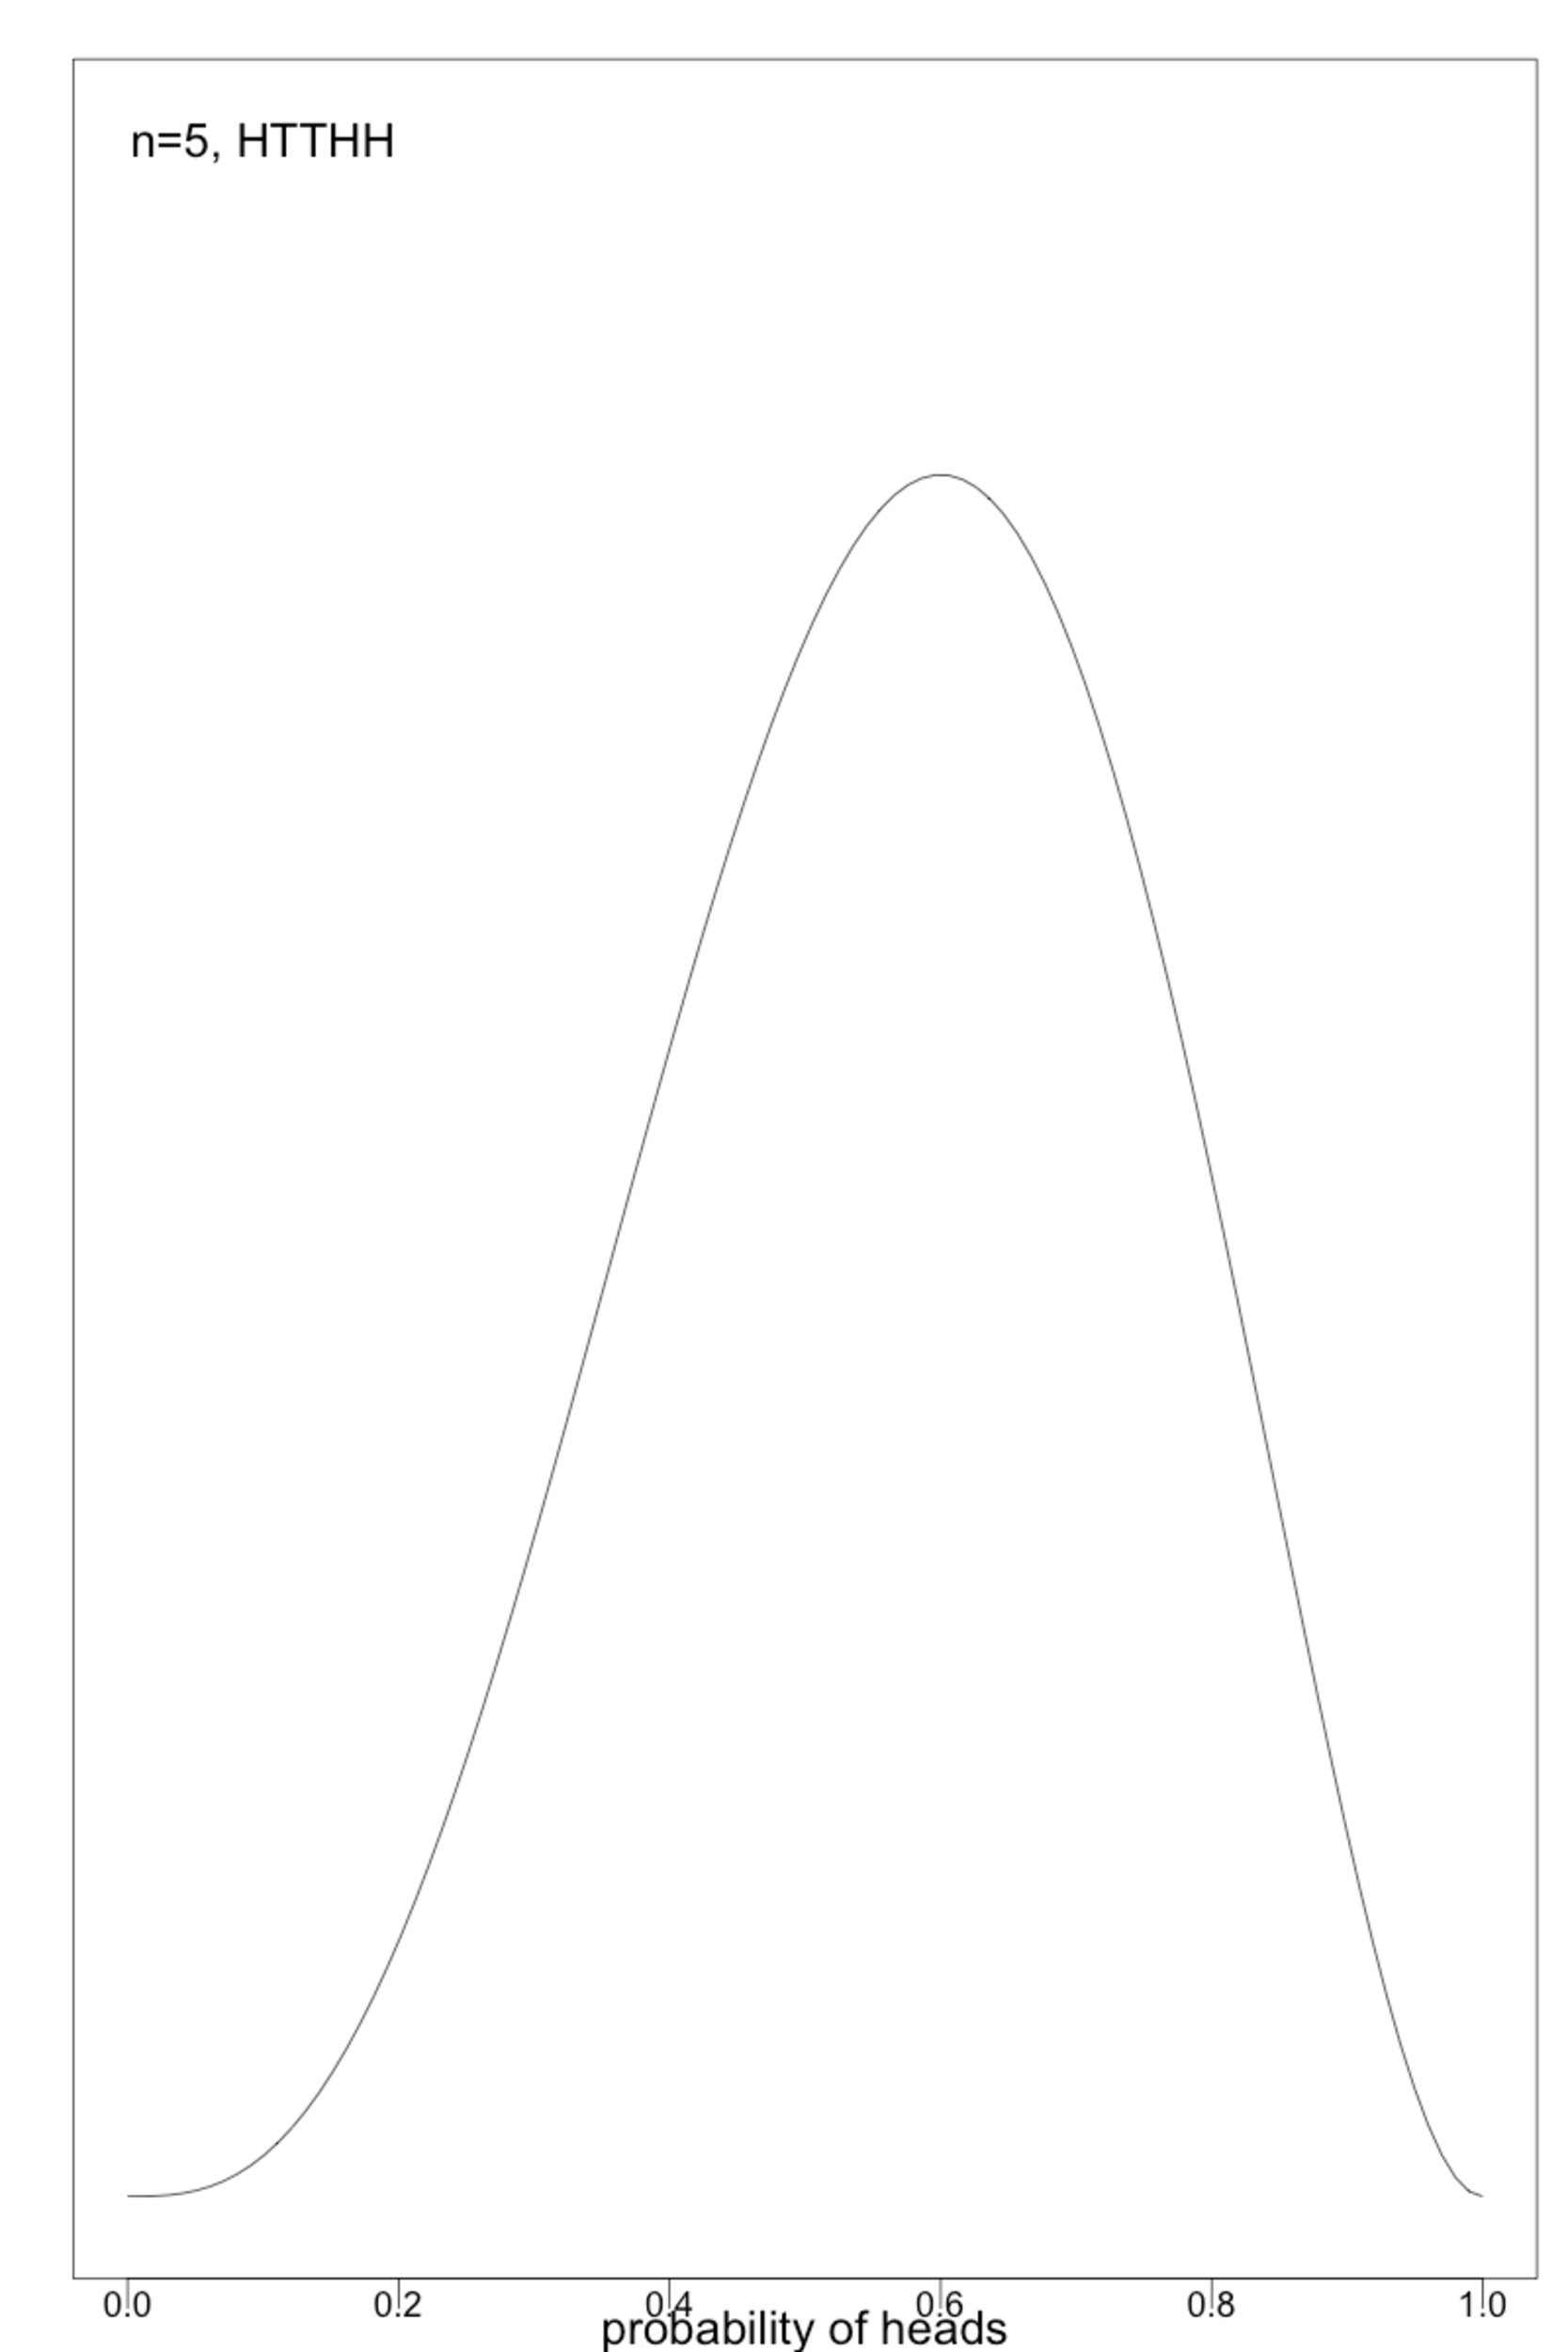
\includegraphics[width=100pt]{cointosses/Five.pdf}	\pause
%%    	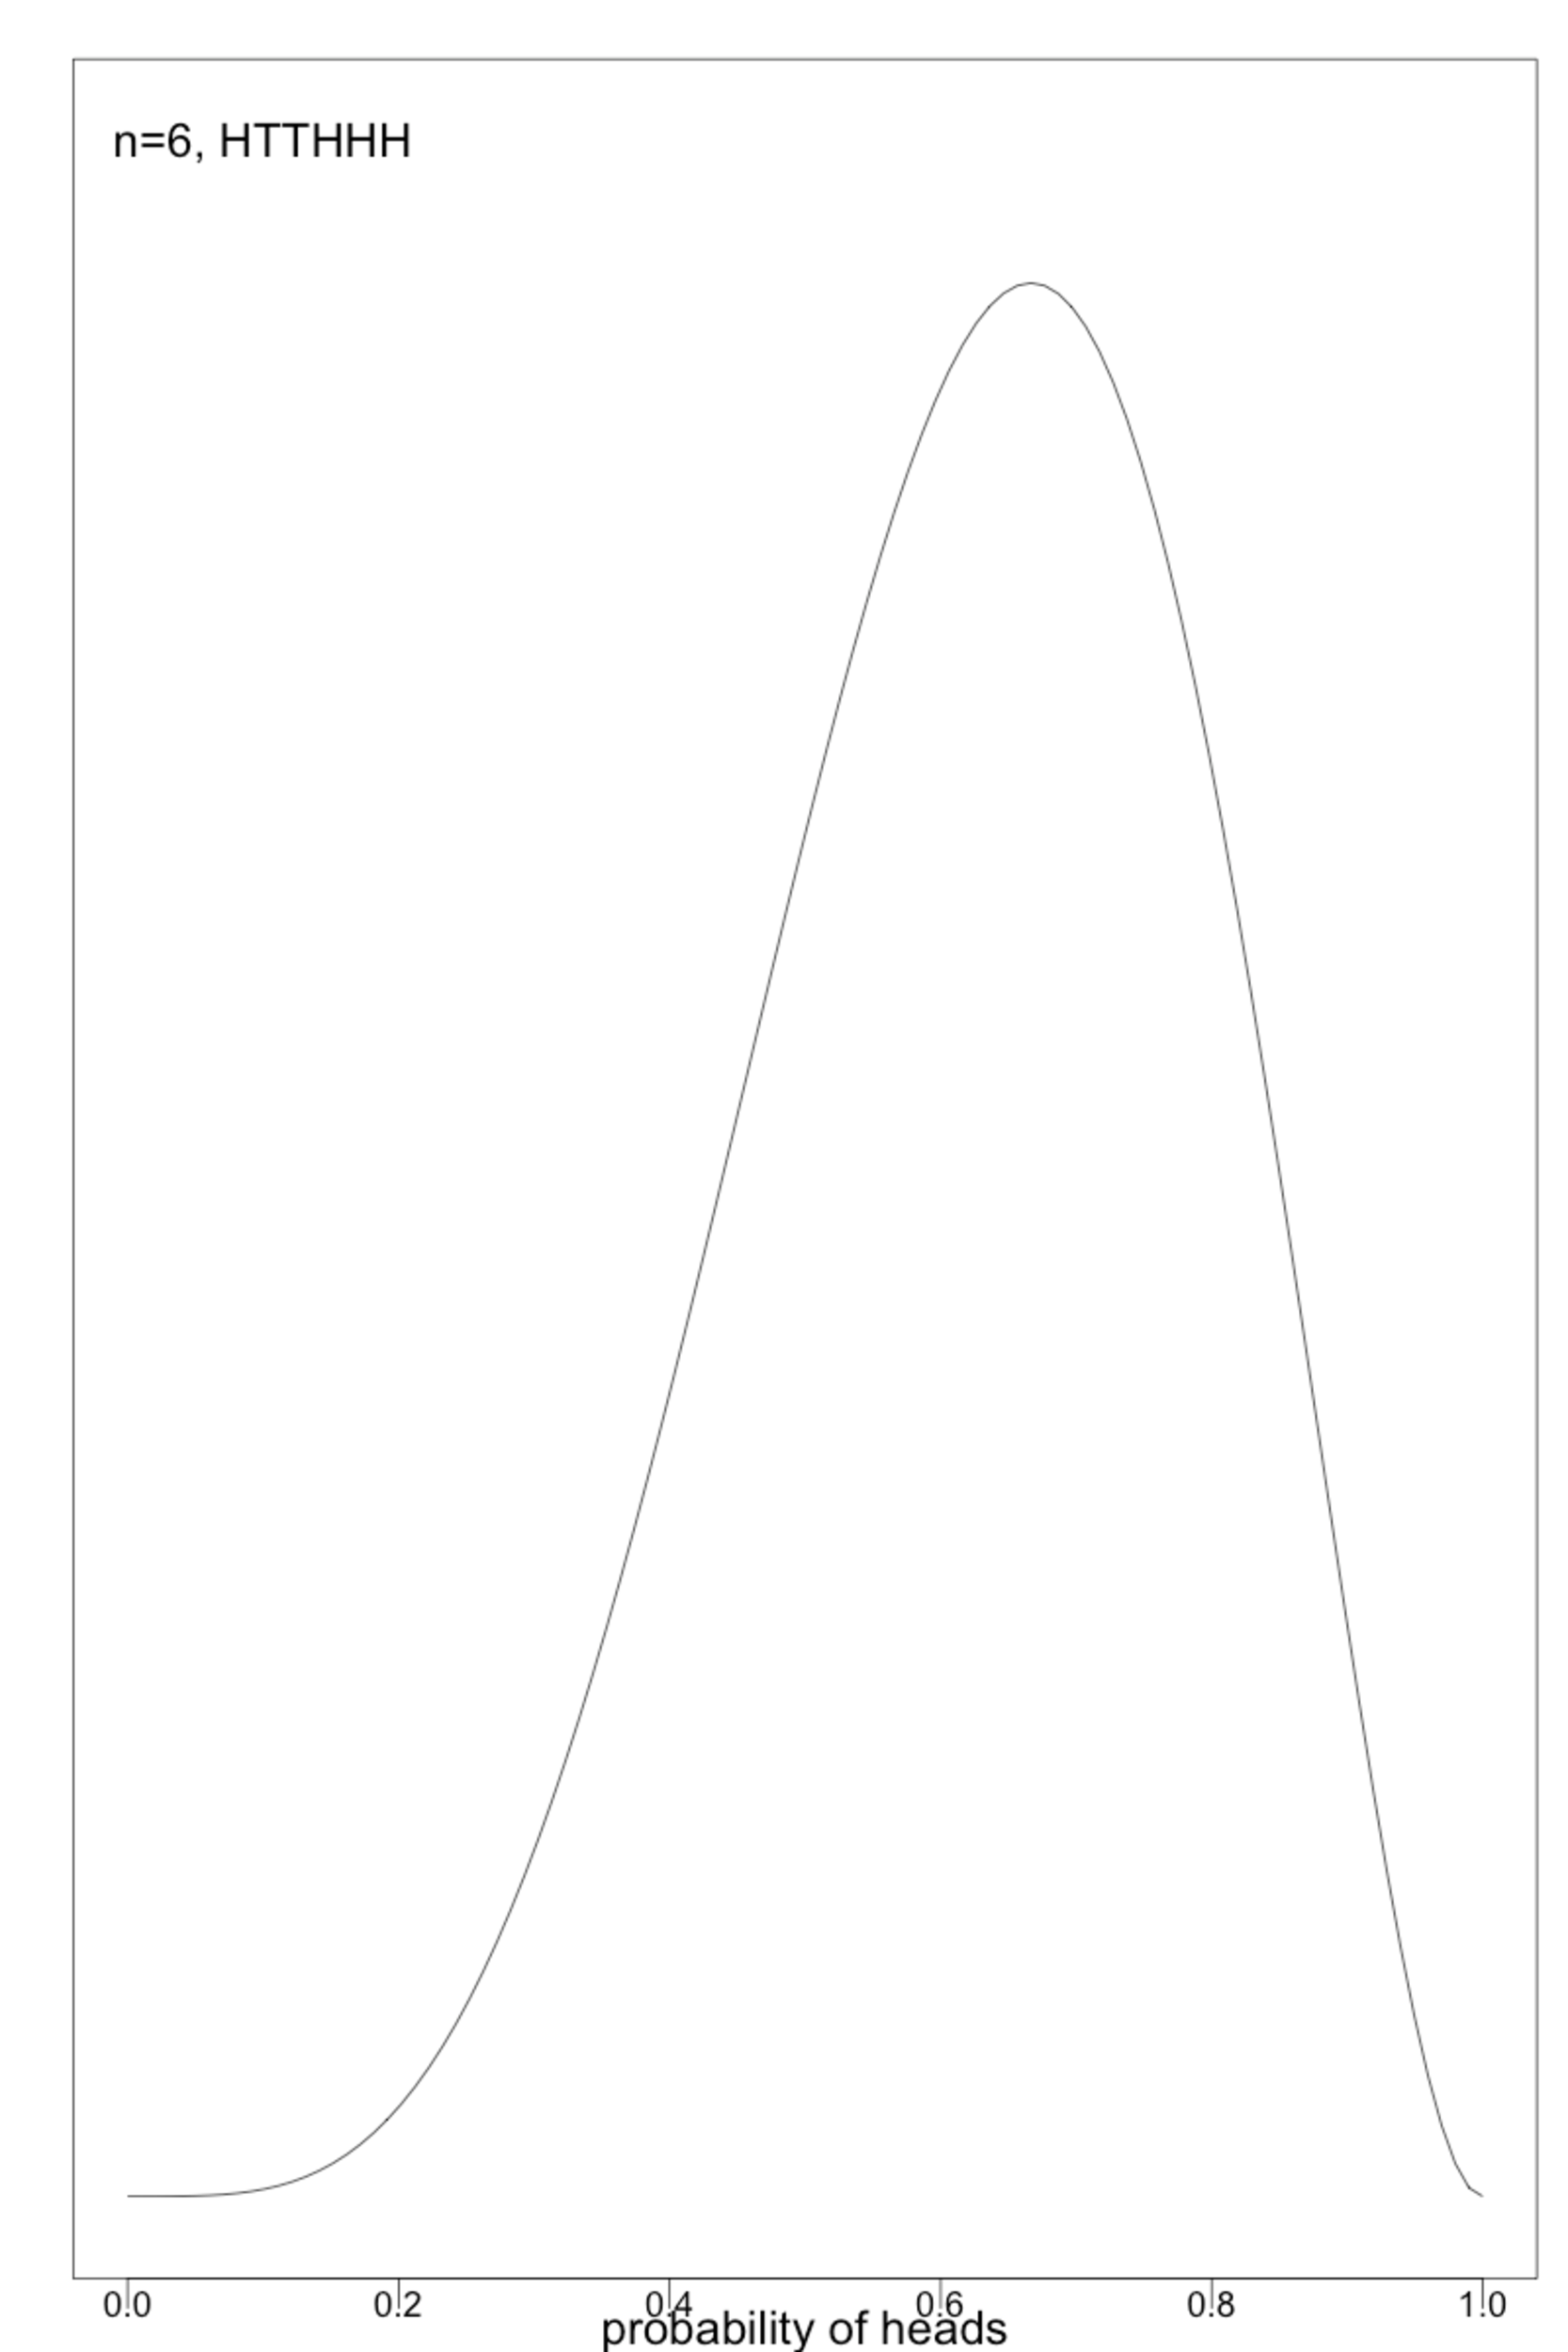
\includegraphics[width=100pt]{cointosses/Six.pdf} 
%%\end{frame}
%%
%%\begin{frame}{Ten Coin Tosses}
%%    	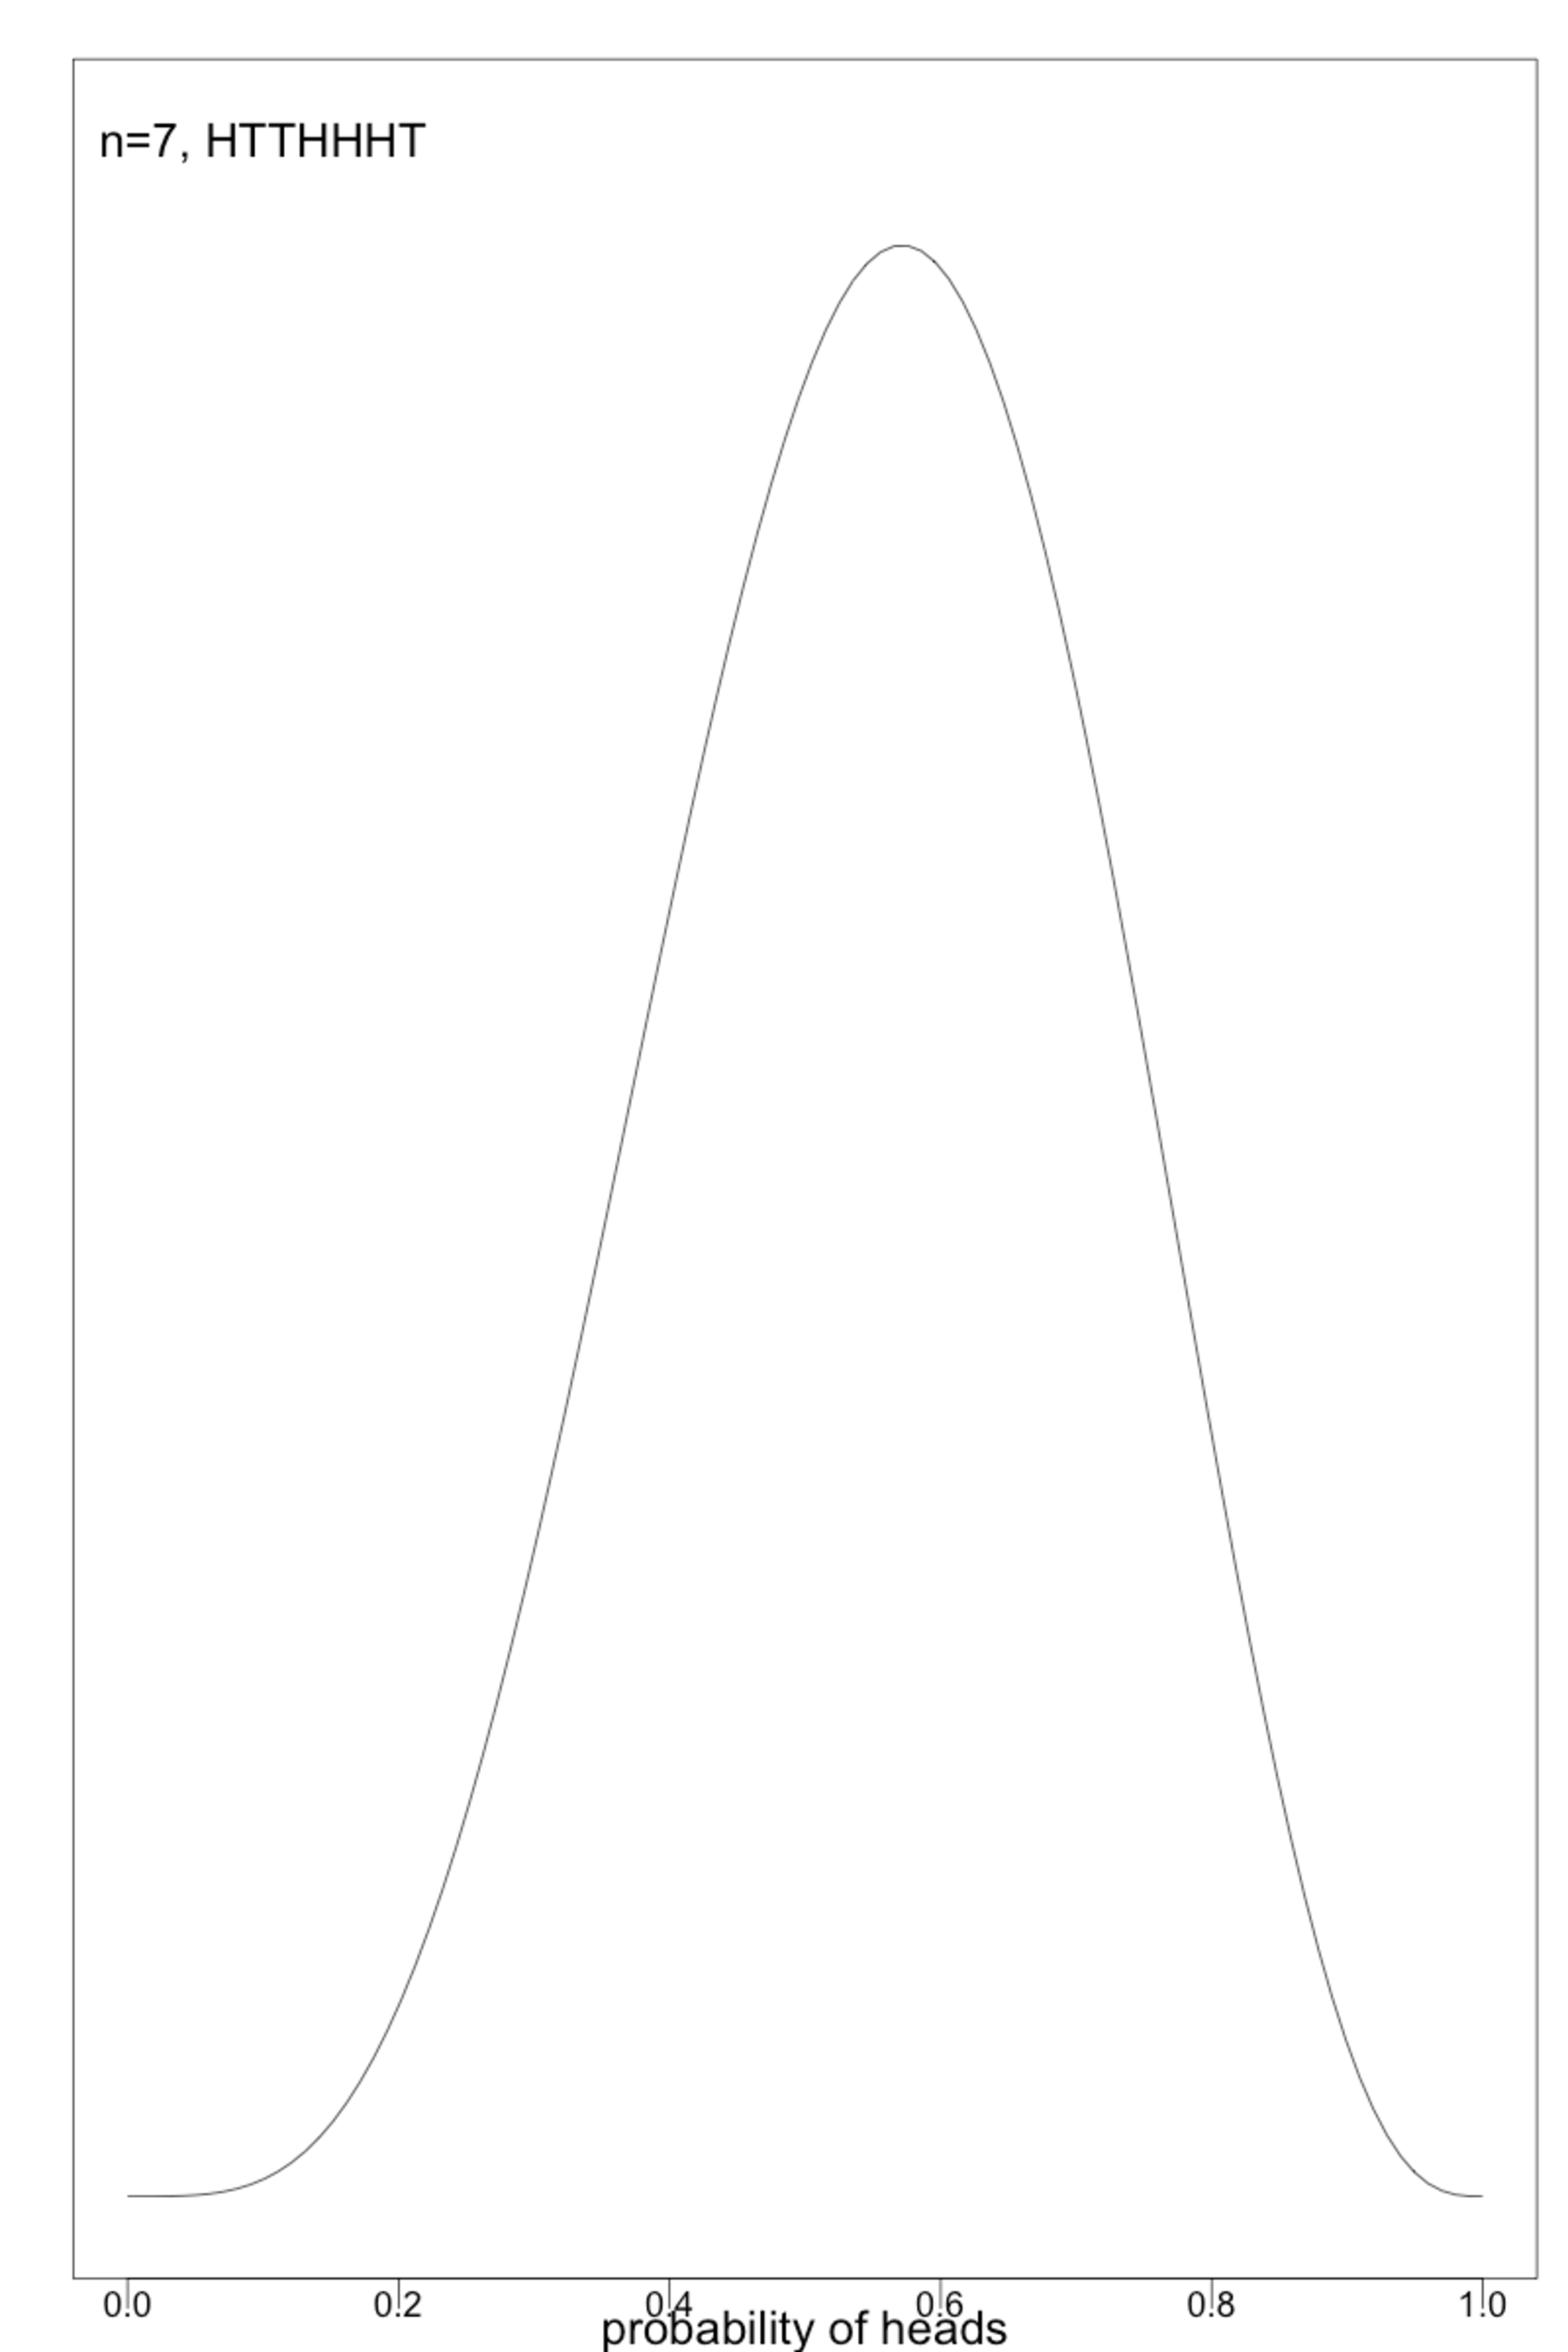
\includegraphics[width=100pt]{cointosses/Seven.pdf}\pause
%%    	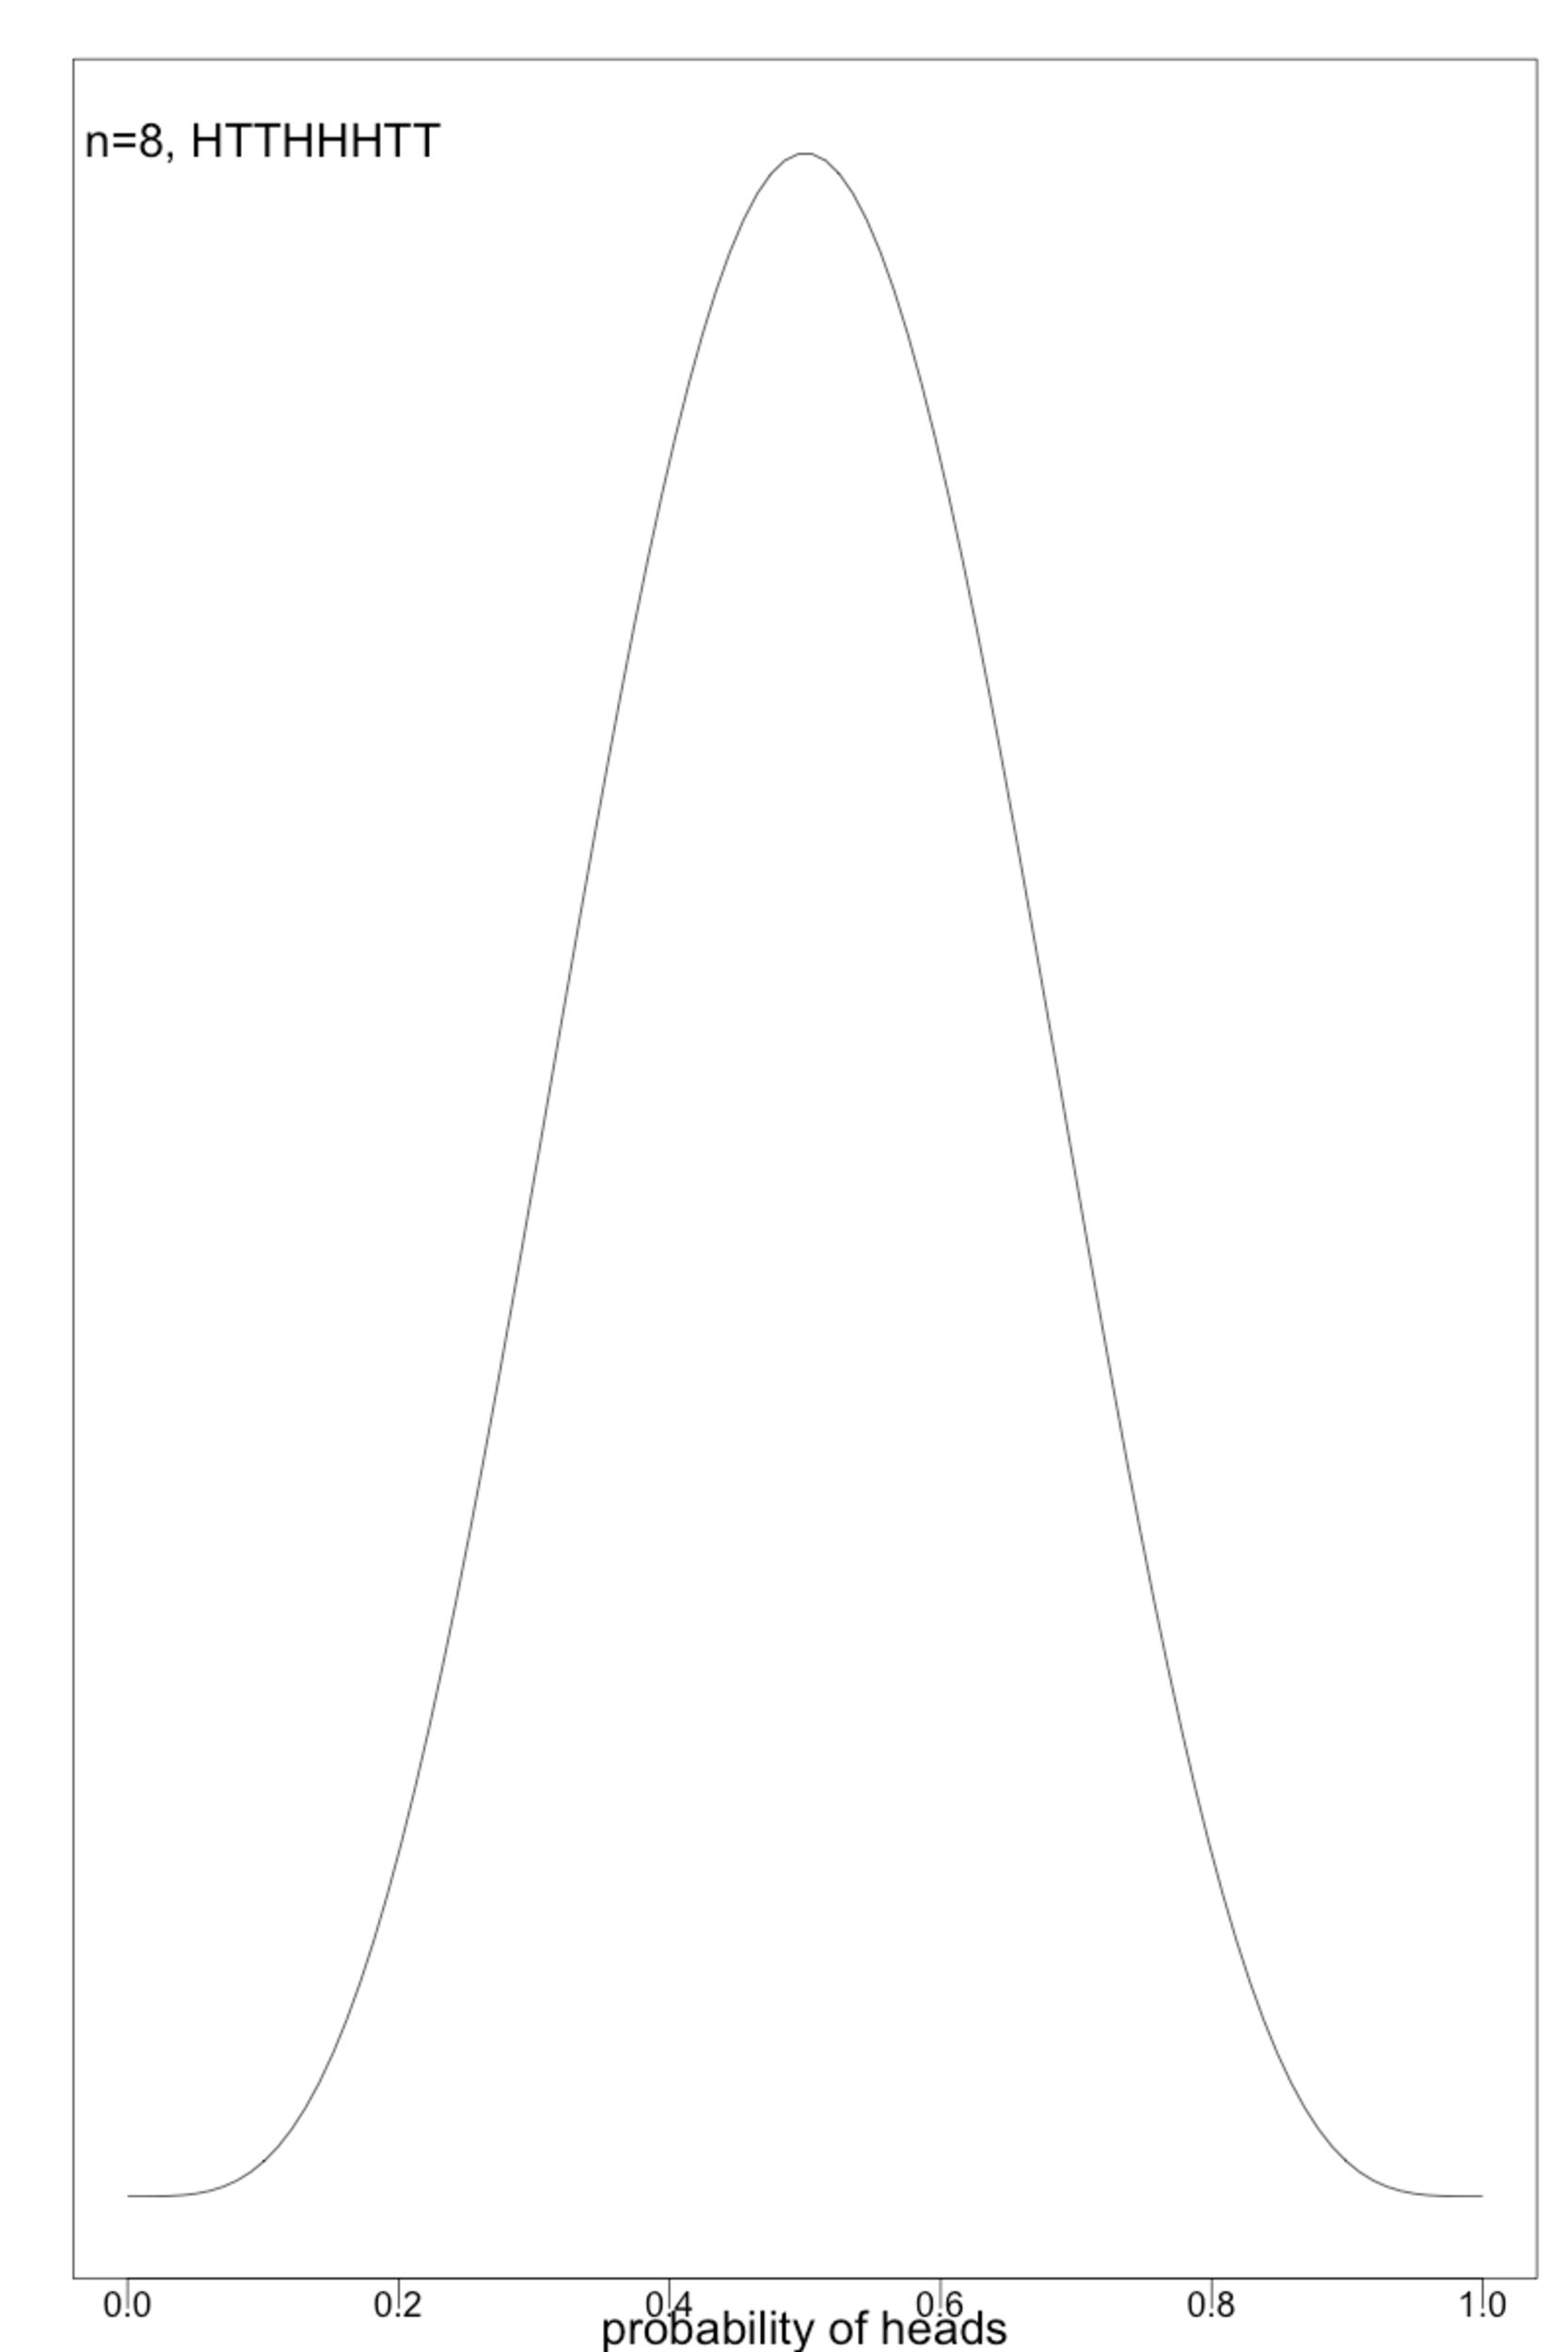
\includegraphics[width=100pt]{cointosses/Eight.pdf}	\pause
%%    	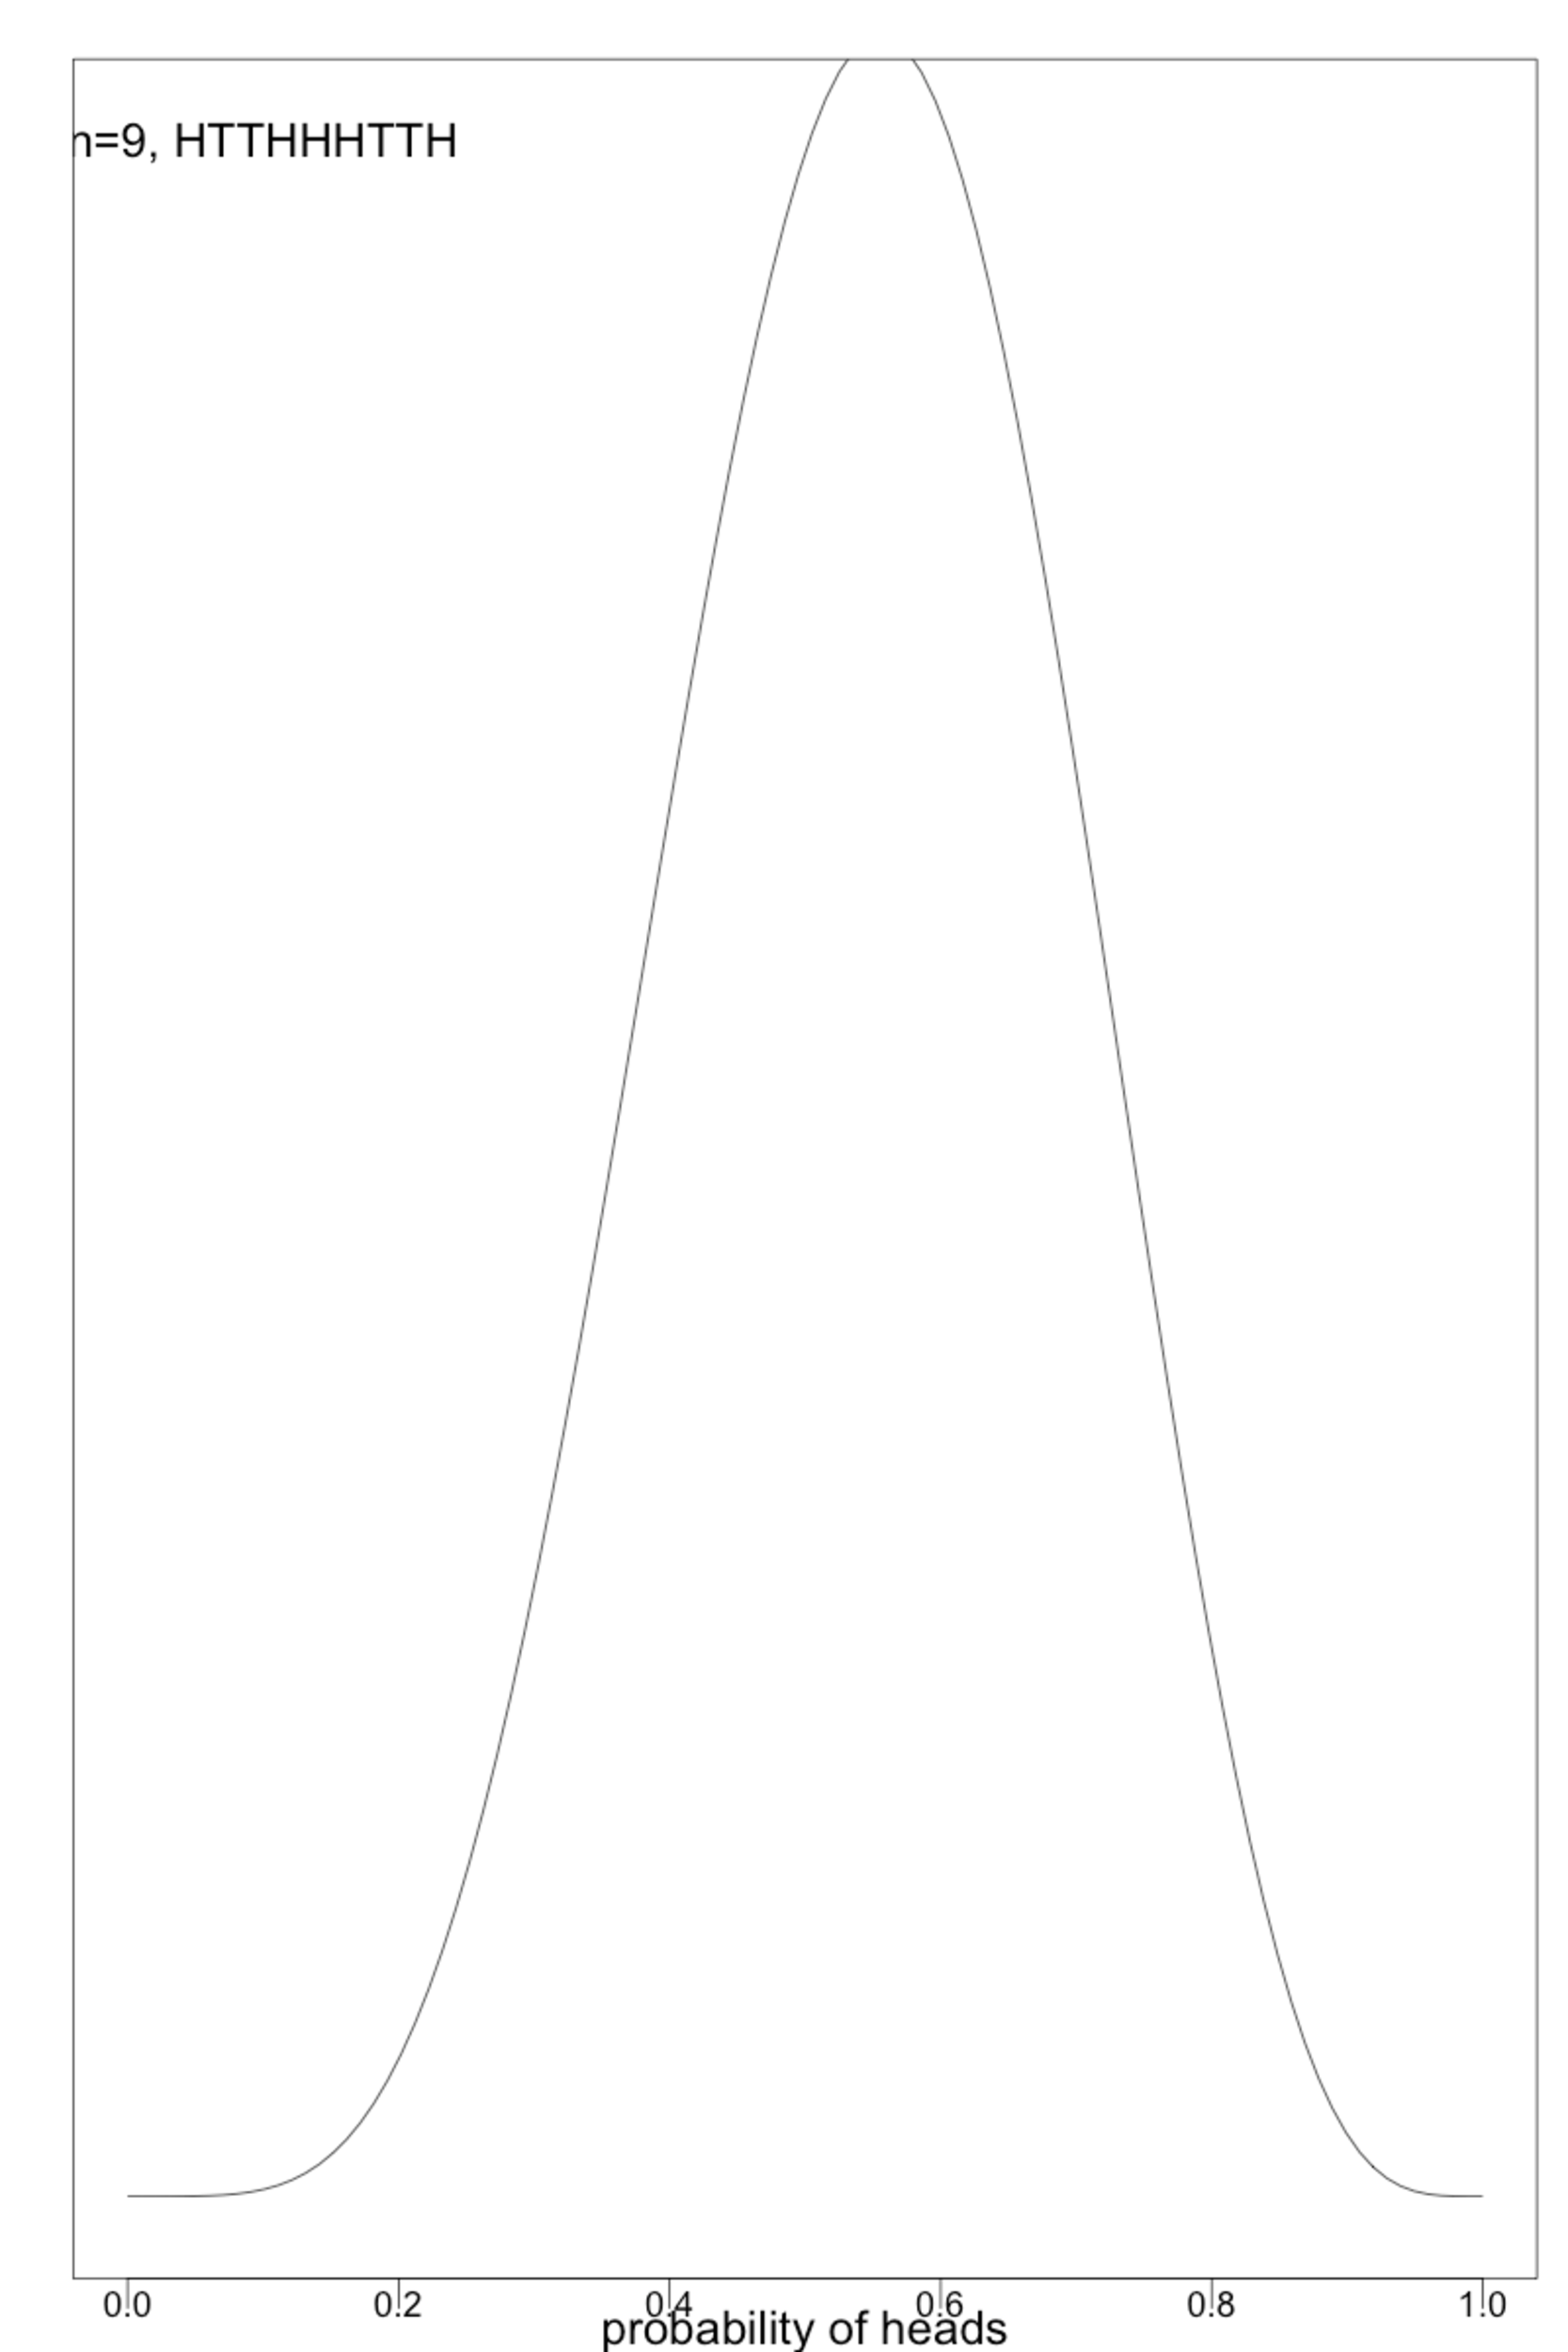
\includegraphics[width=100pt]{cointosses/Nine.pdf}
%%\end{frame}
%%
%%\begin{frame}{Ten Coin Tosses}
%%	 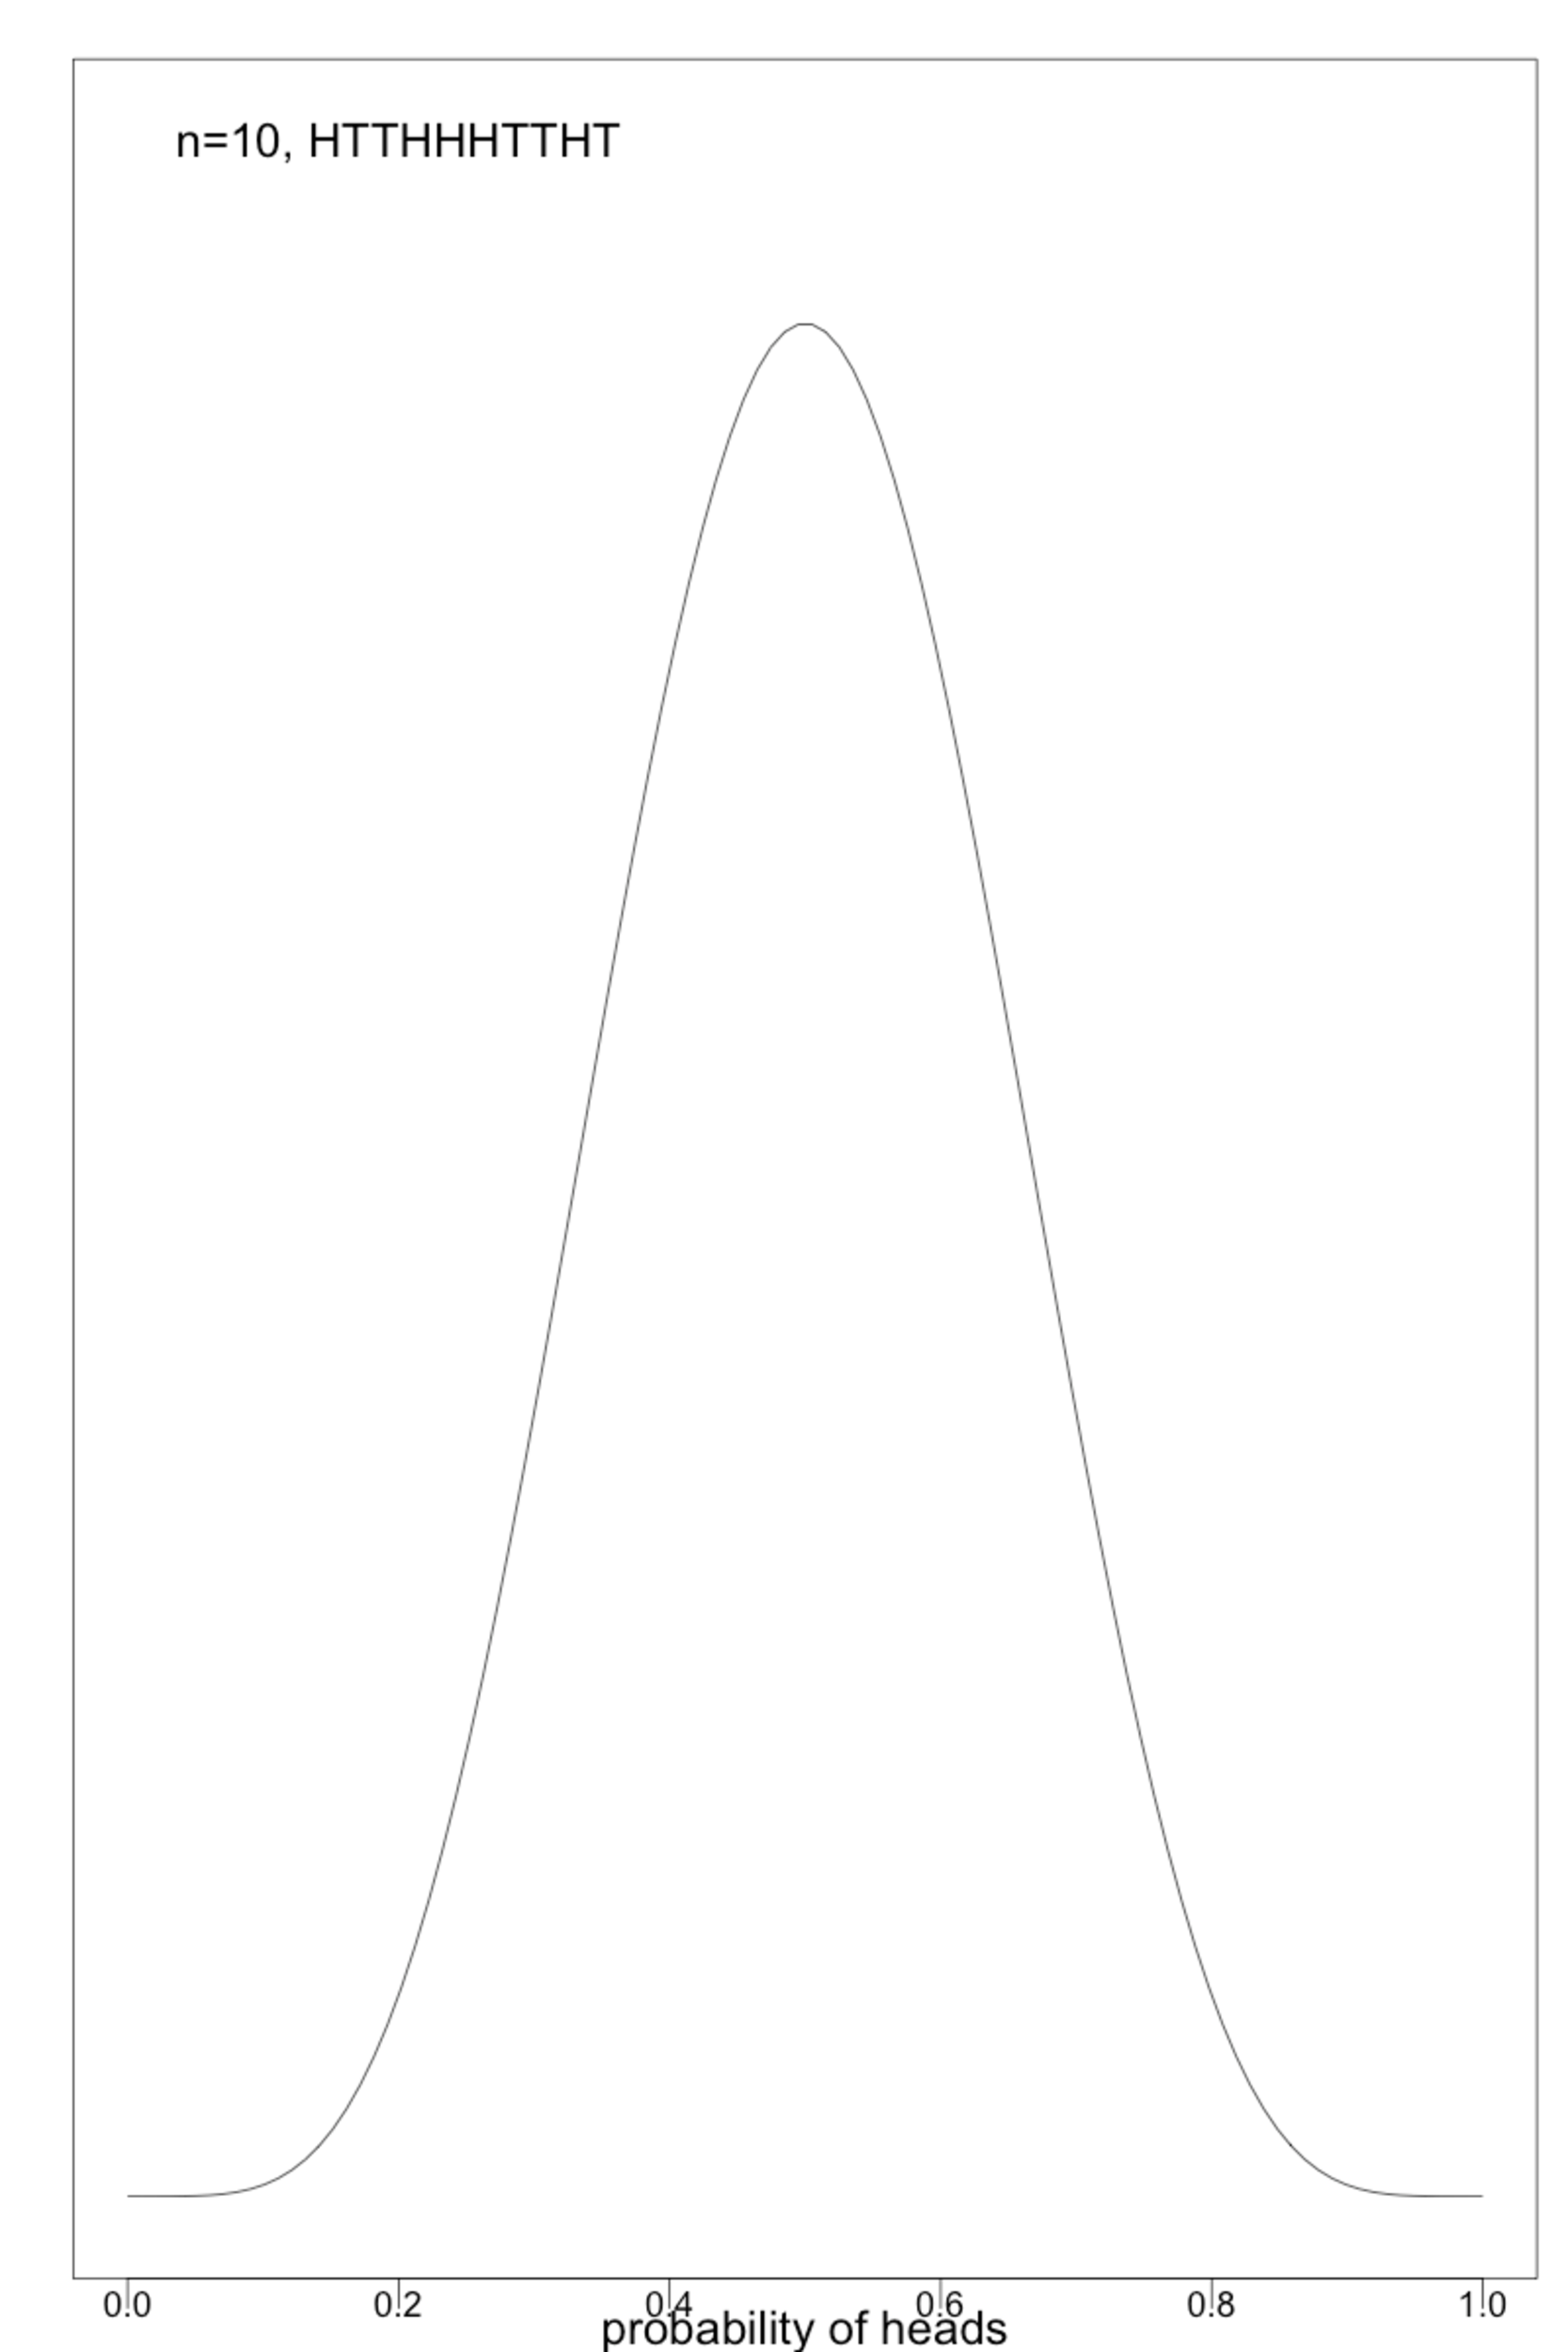
\includegraphics[width=100pt]{cointosses/Ten.pdf}
%%\end{frame}
%%
%%
%%\begin{frame}{Ten Coin Tosses}{Some Other Priors}
%%		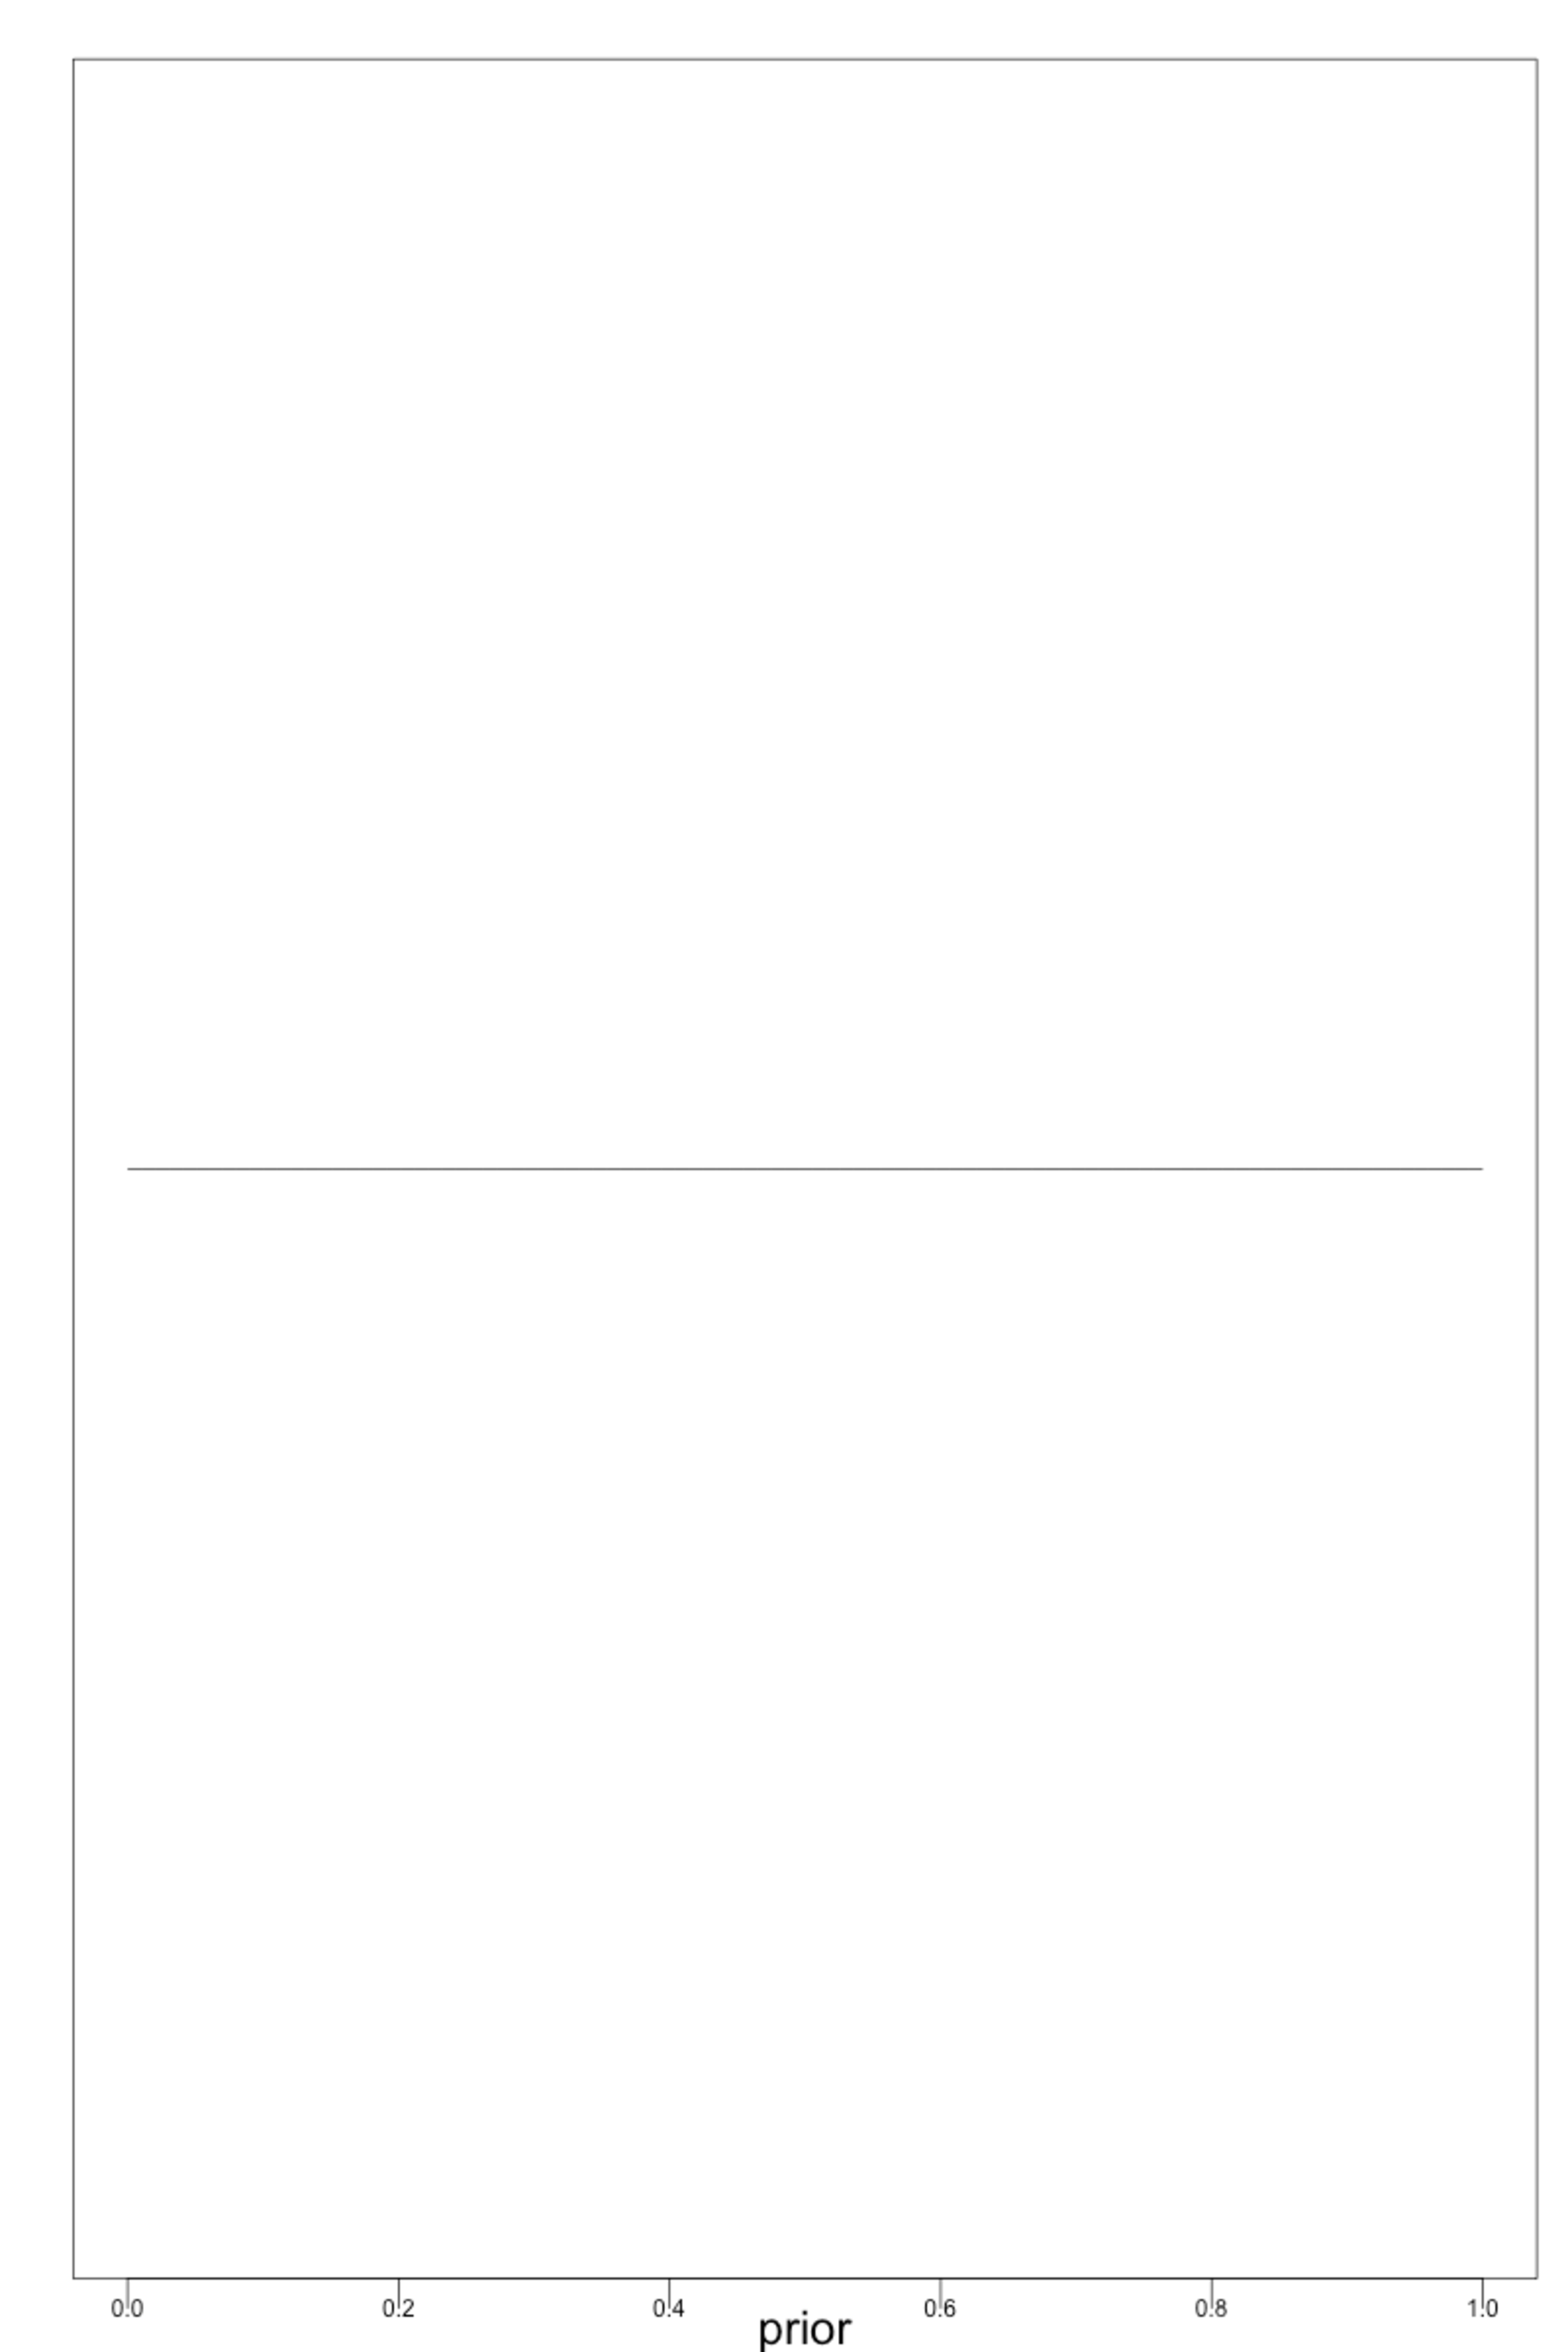
\includegraphics[valign=m, width=100pt]{cointosses/uniform_prior.pdf} $\times$
%%	    	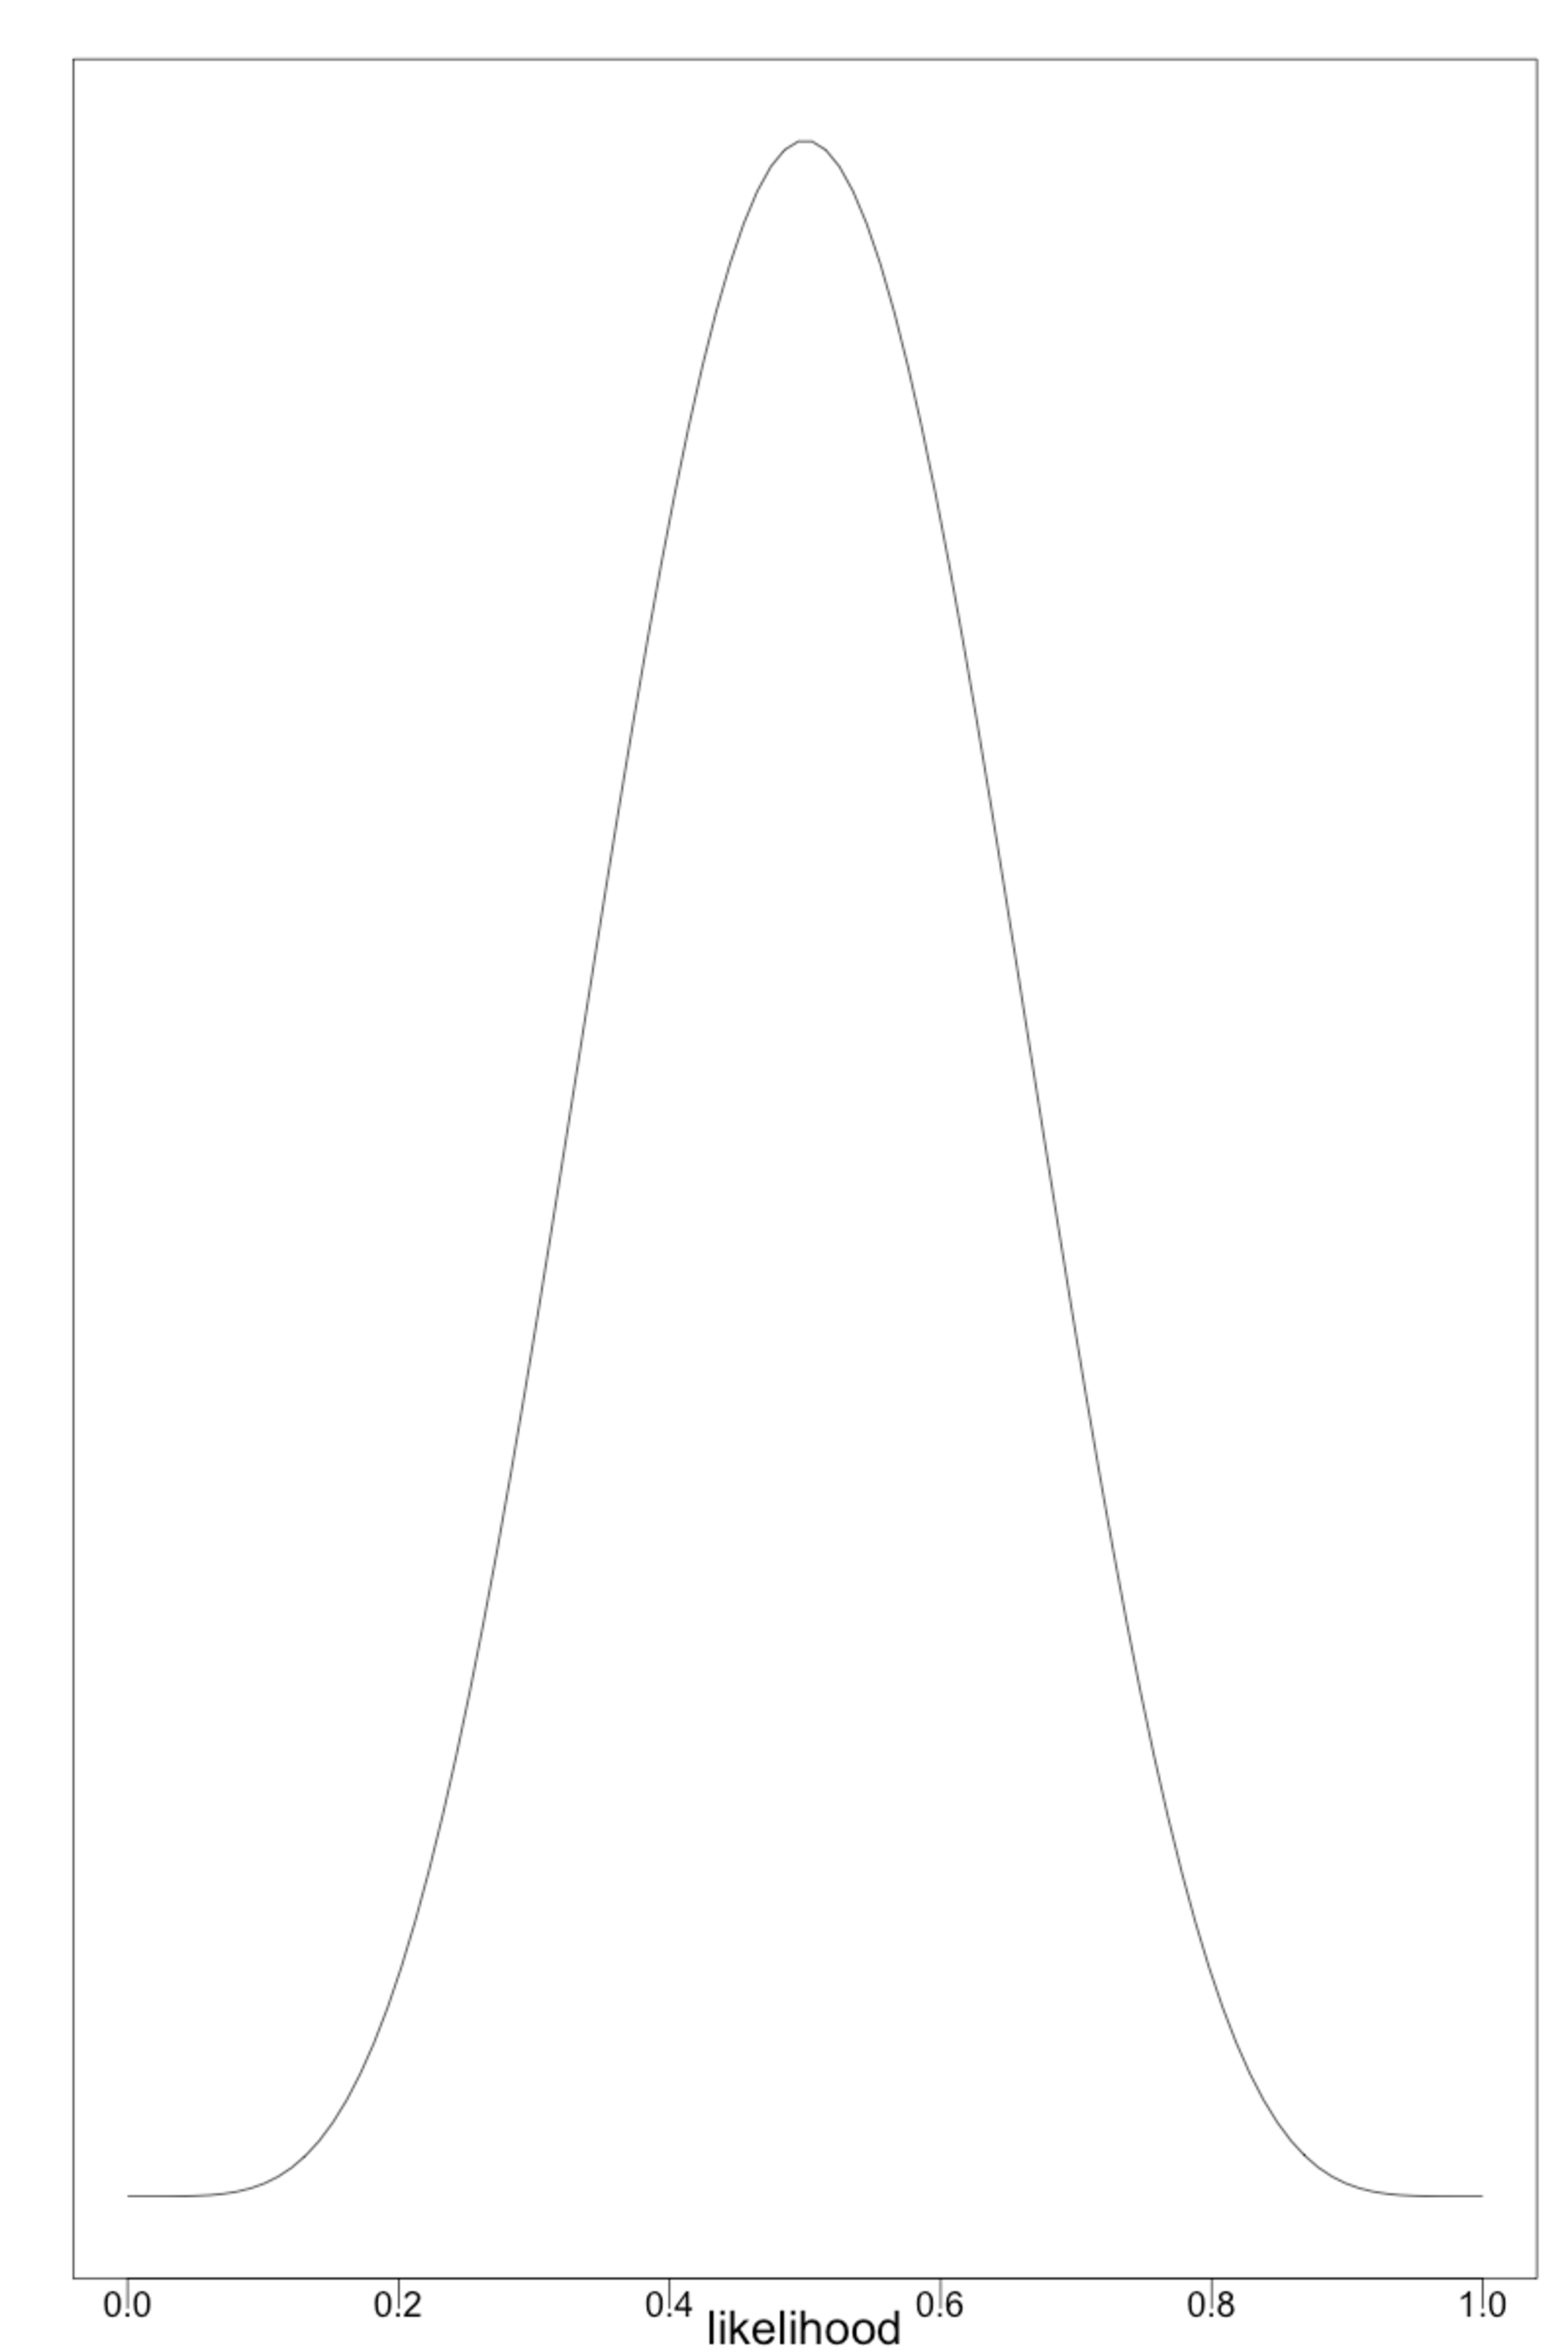
\includegraphics[valign=m, width=100pt]{cointosses/Ten_pre.pdf} $\propto$
%%	    	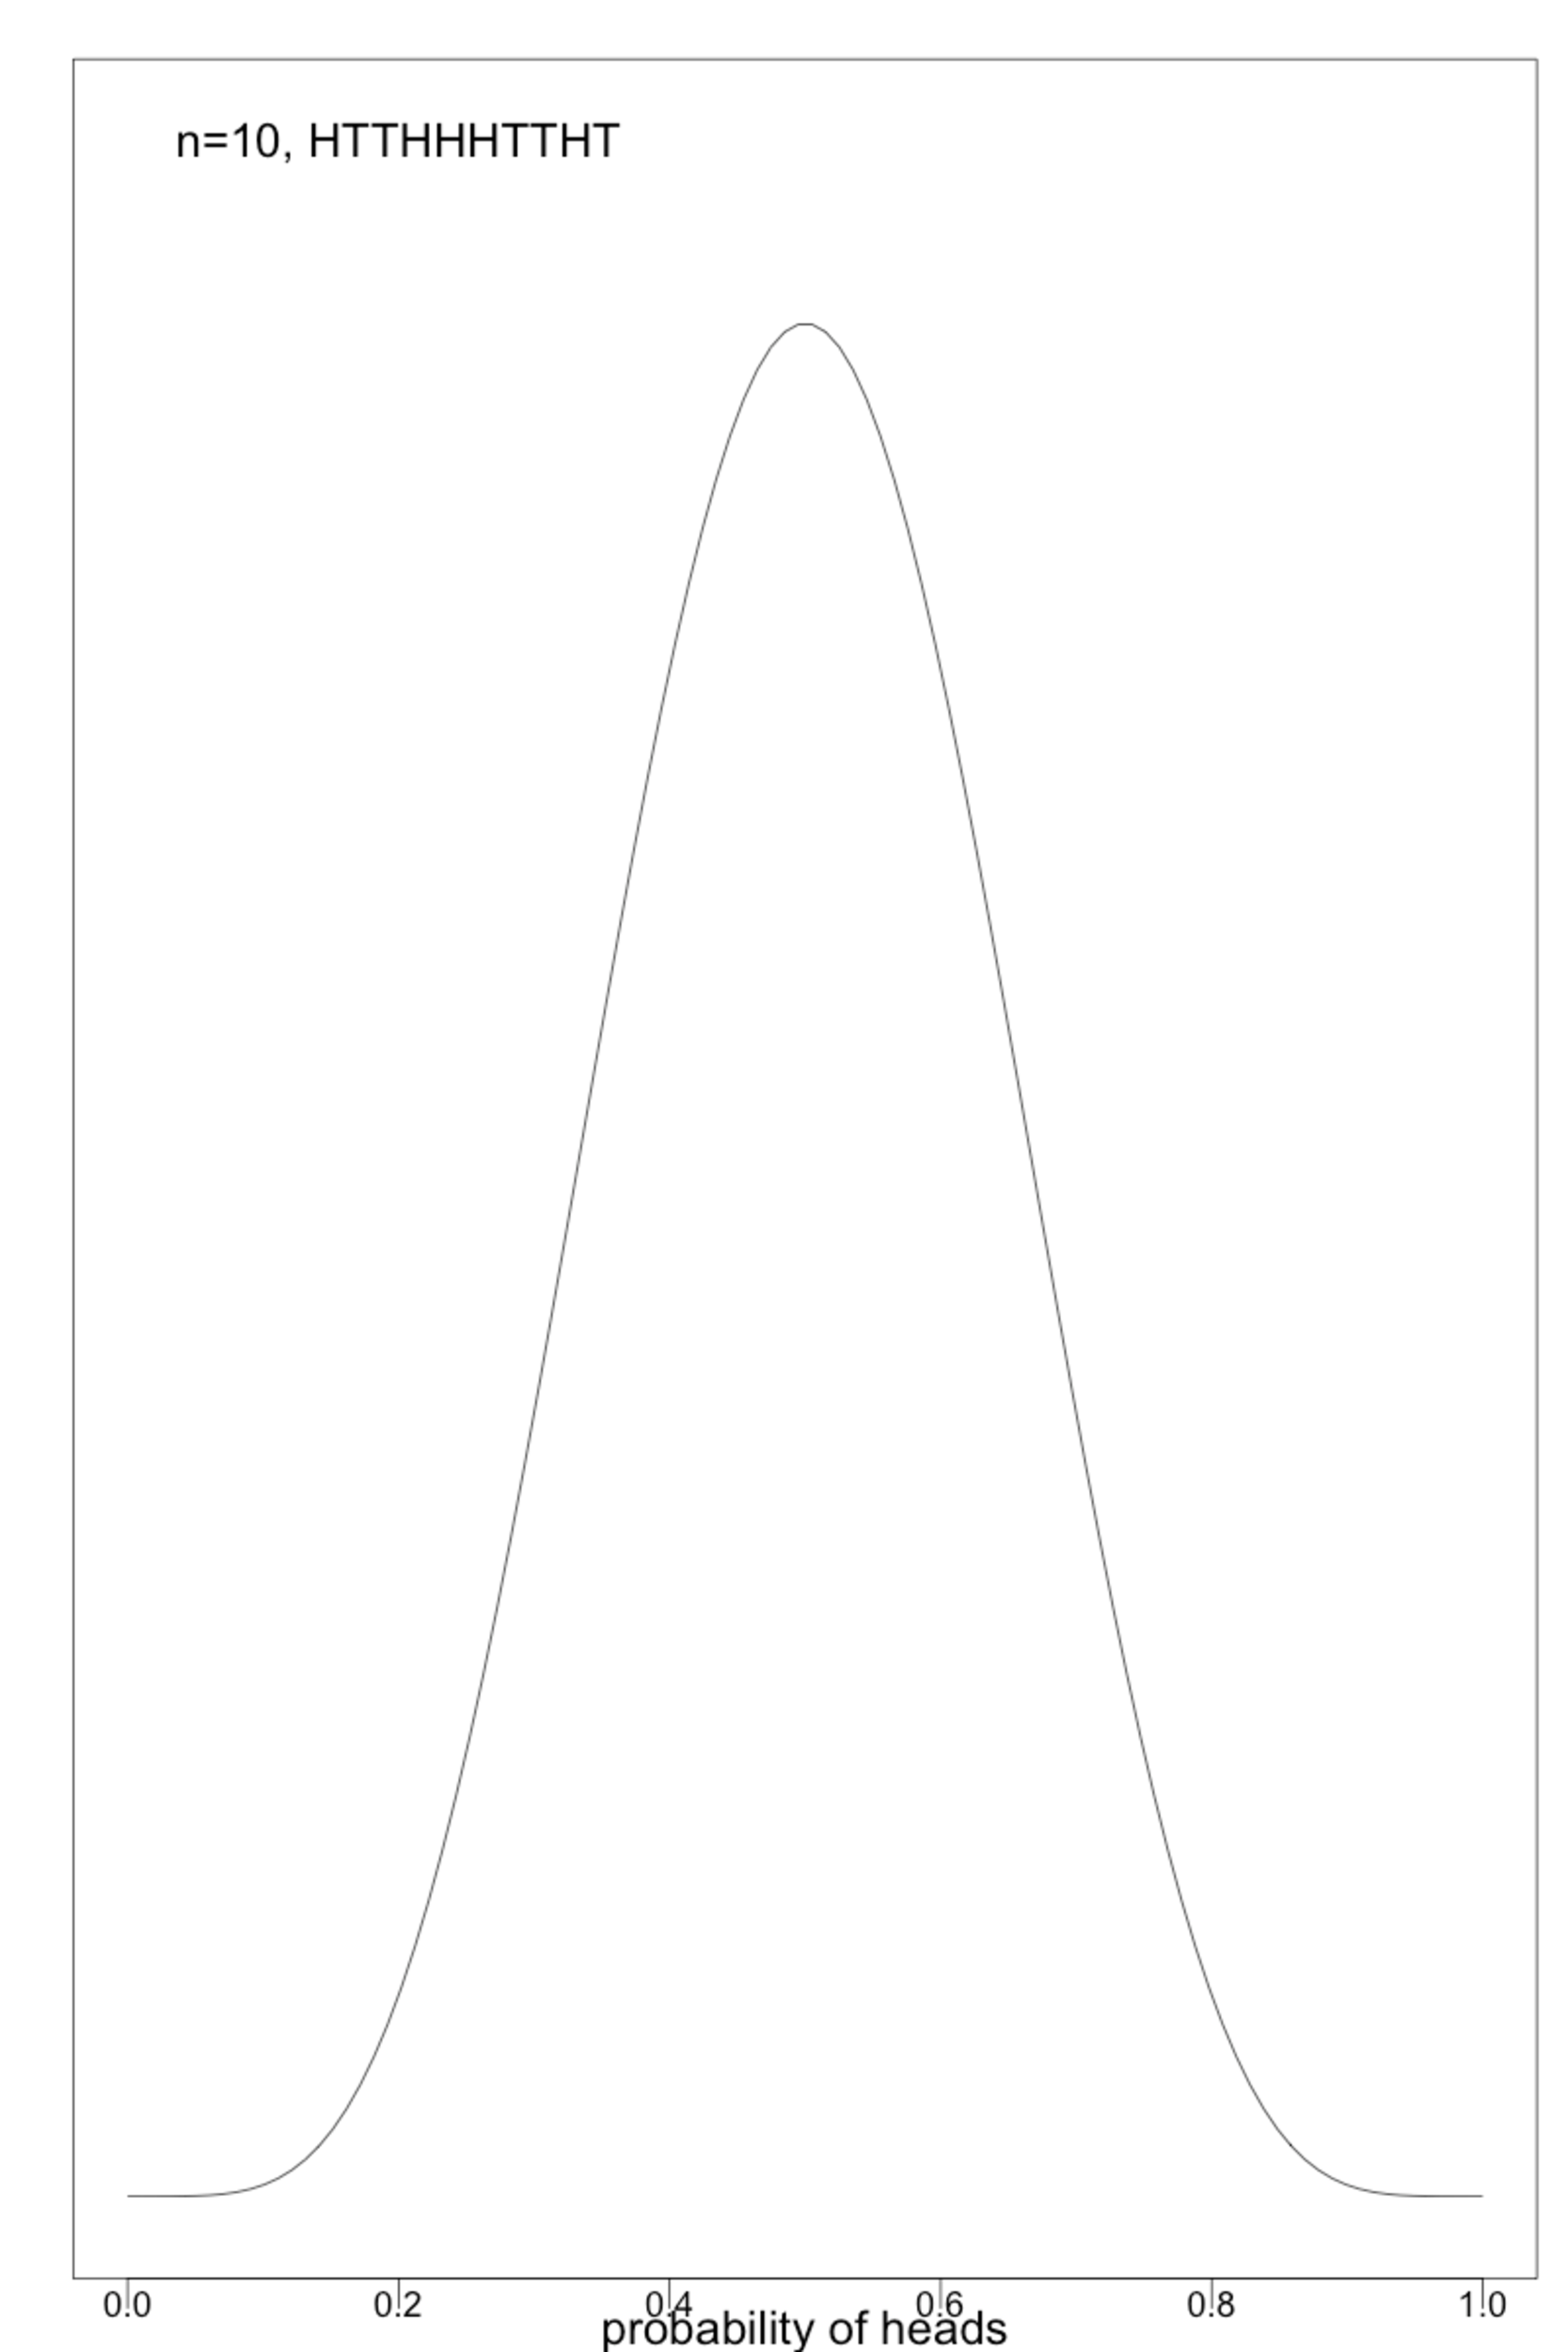
\includegraphics[valign=m, width=100pt]{cointosses/Ten.pdf}
%%\end{frame}
%%
%%\begin{frame}{Ten Coin Tosses}{Some Other Priors}
%%		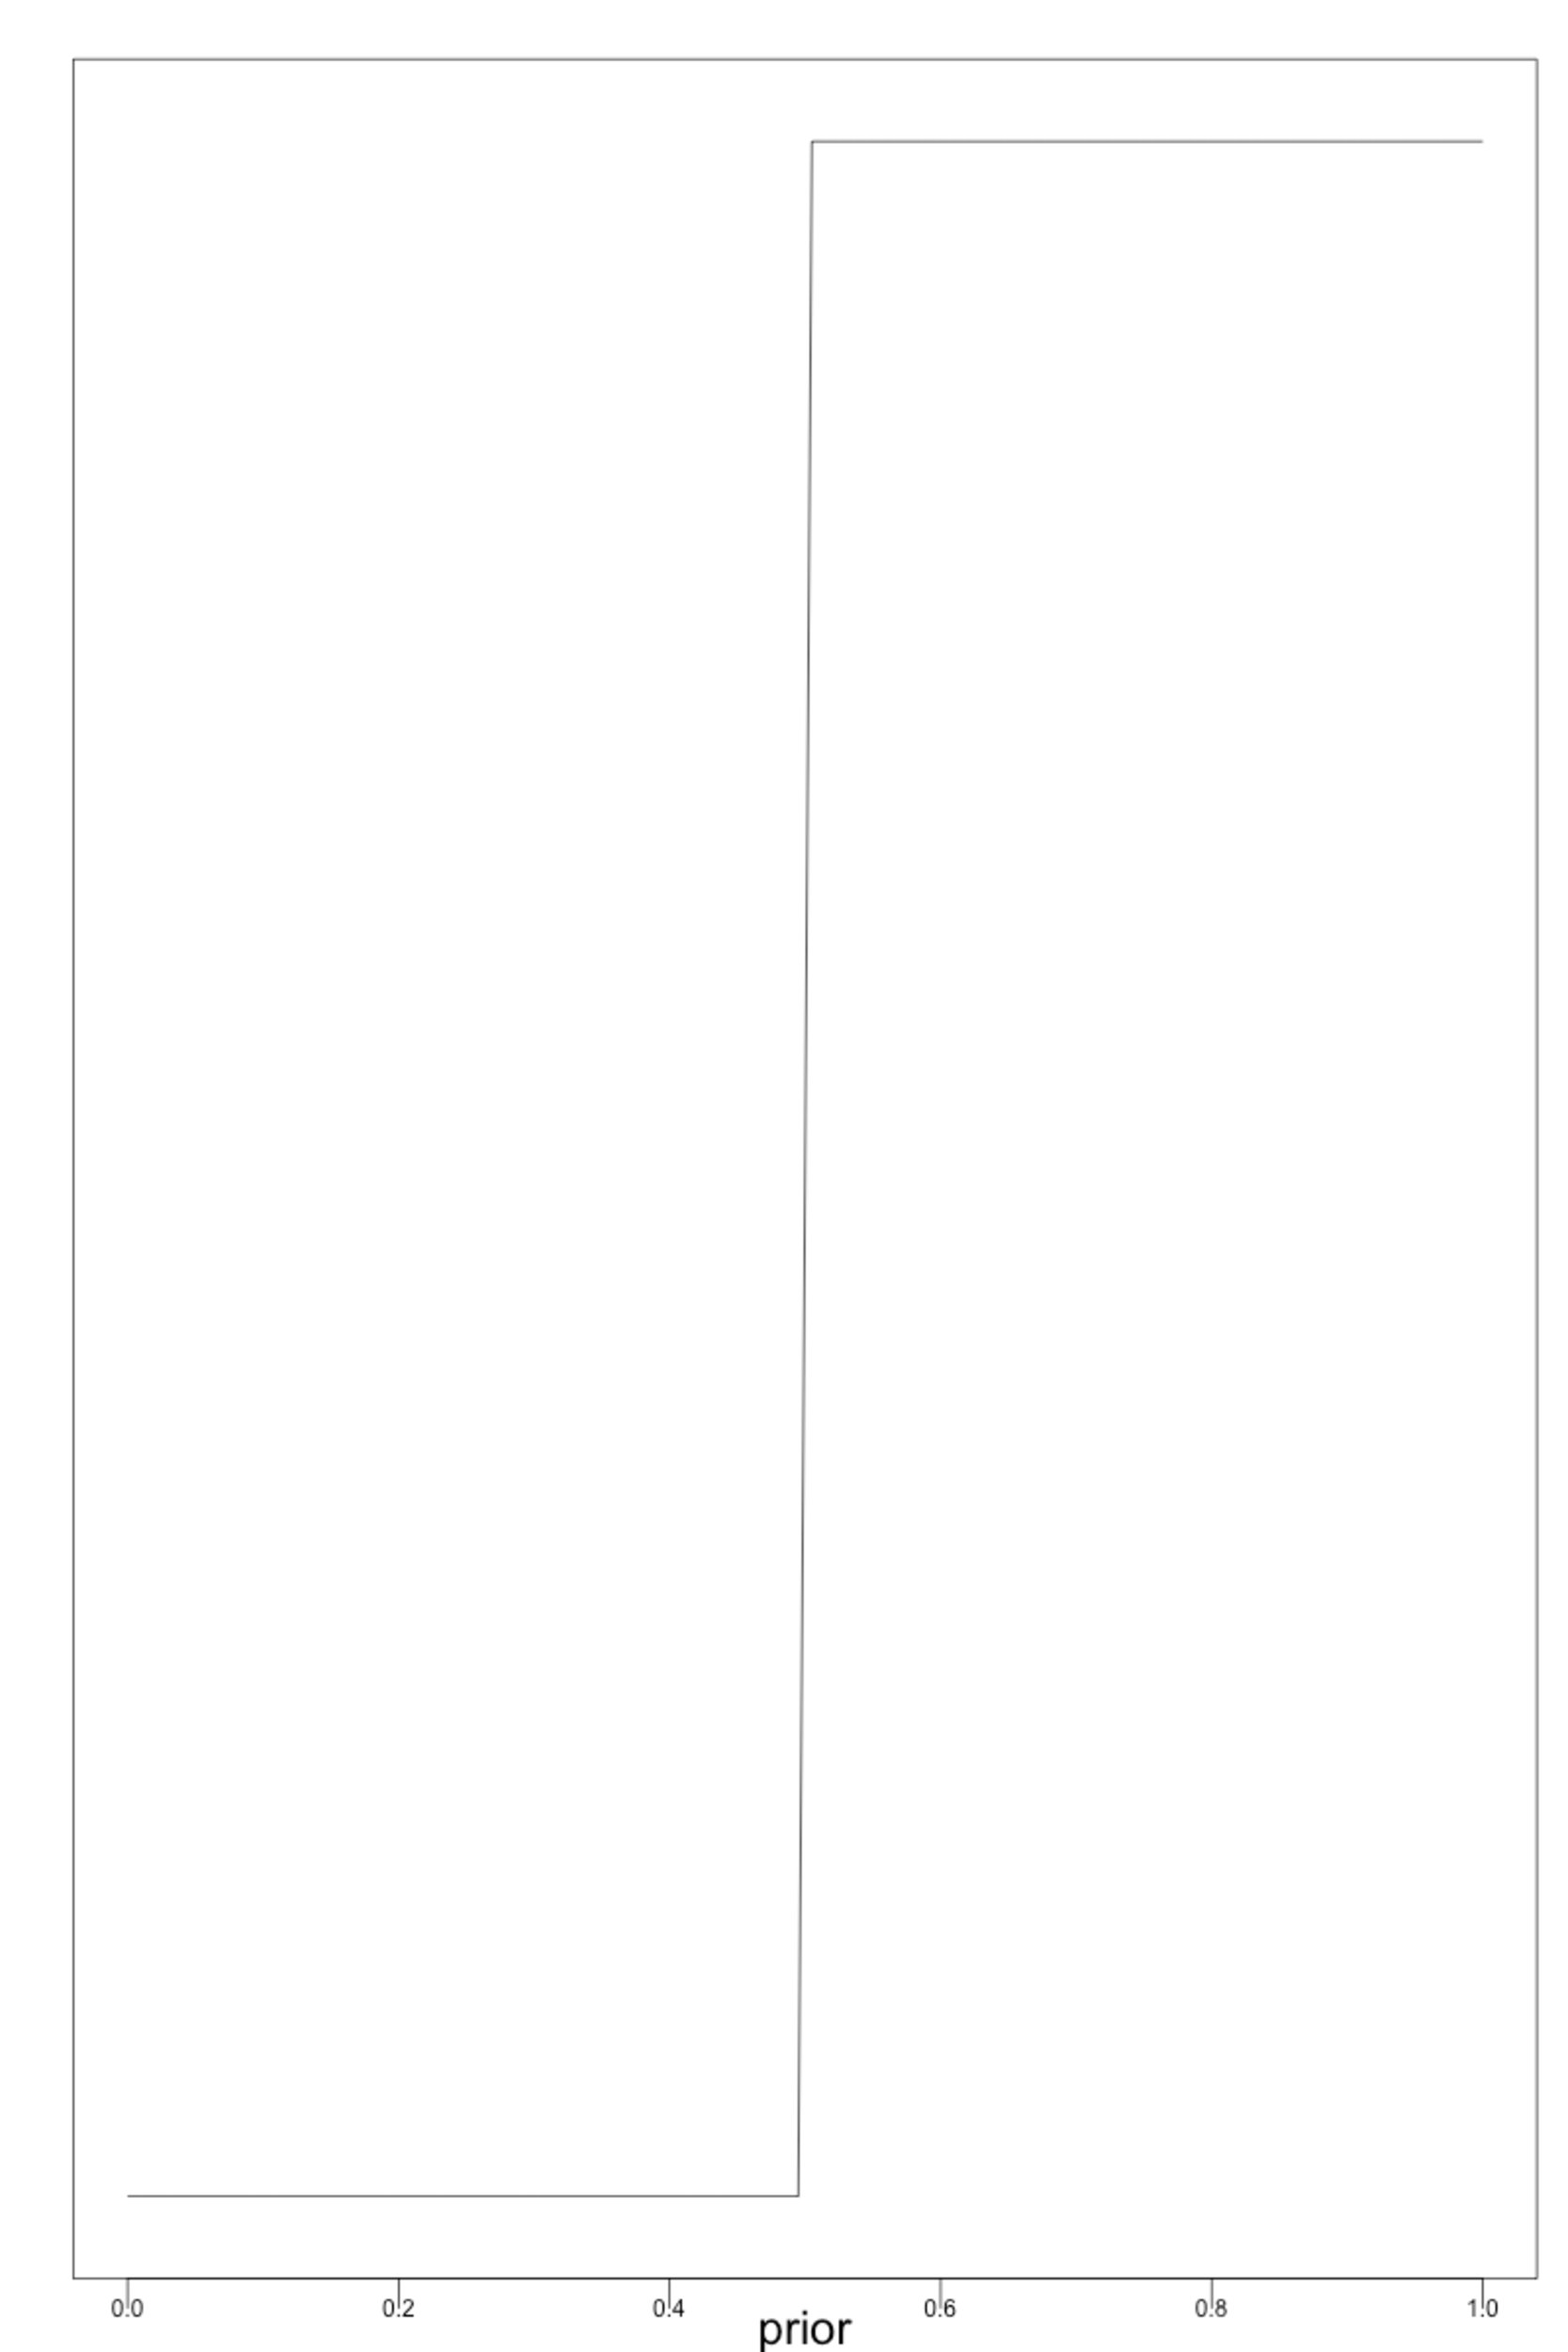
\includegraphics[valign=m, width=100pt]{cointosses/step_prior.pdf} $\times$
%%	    	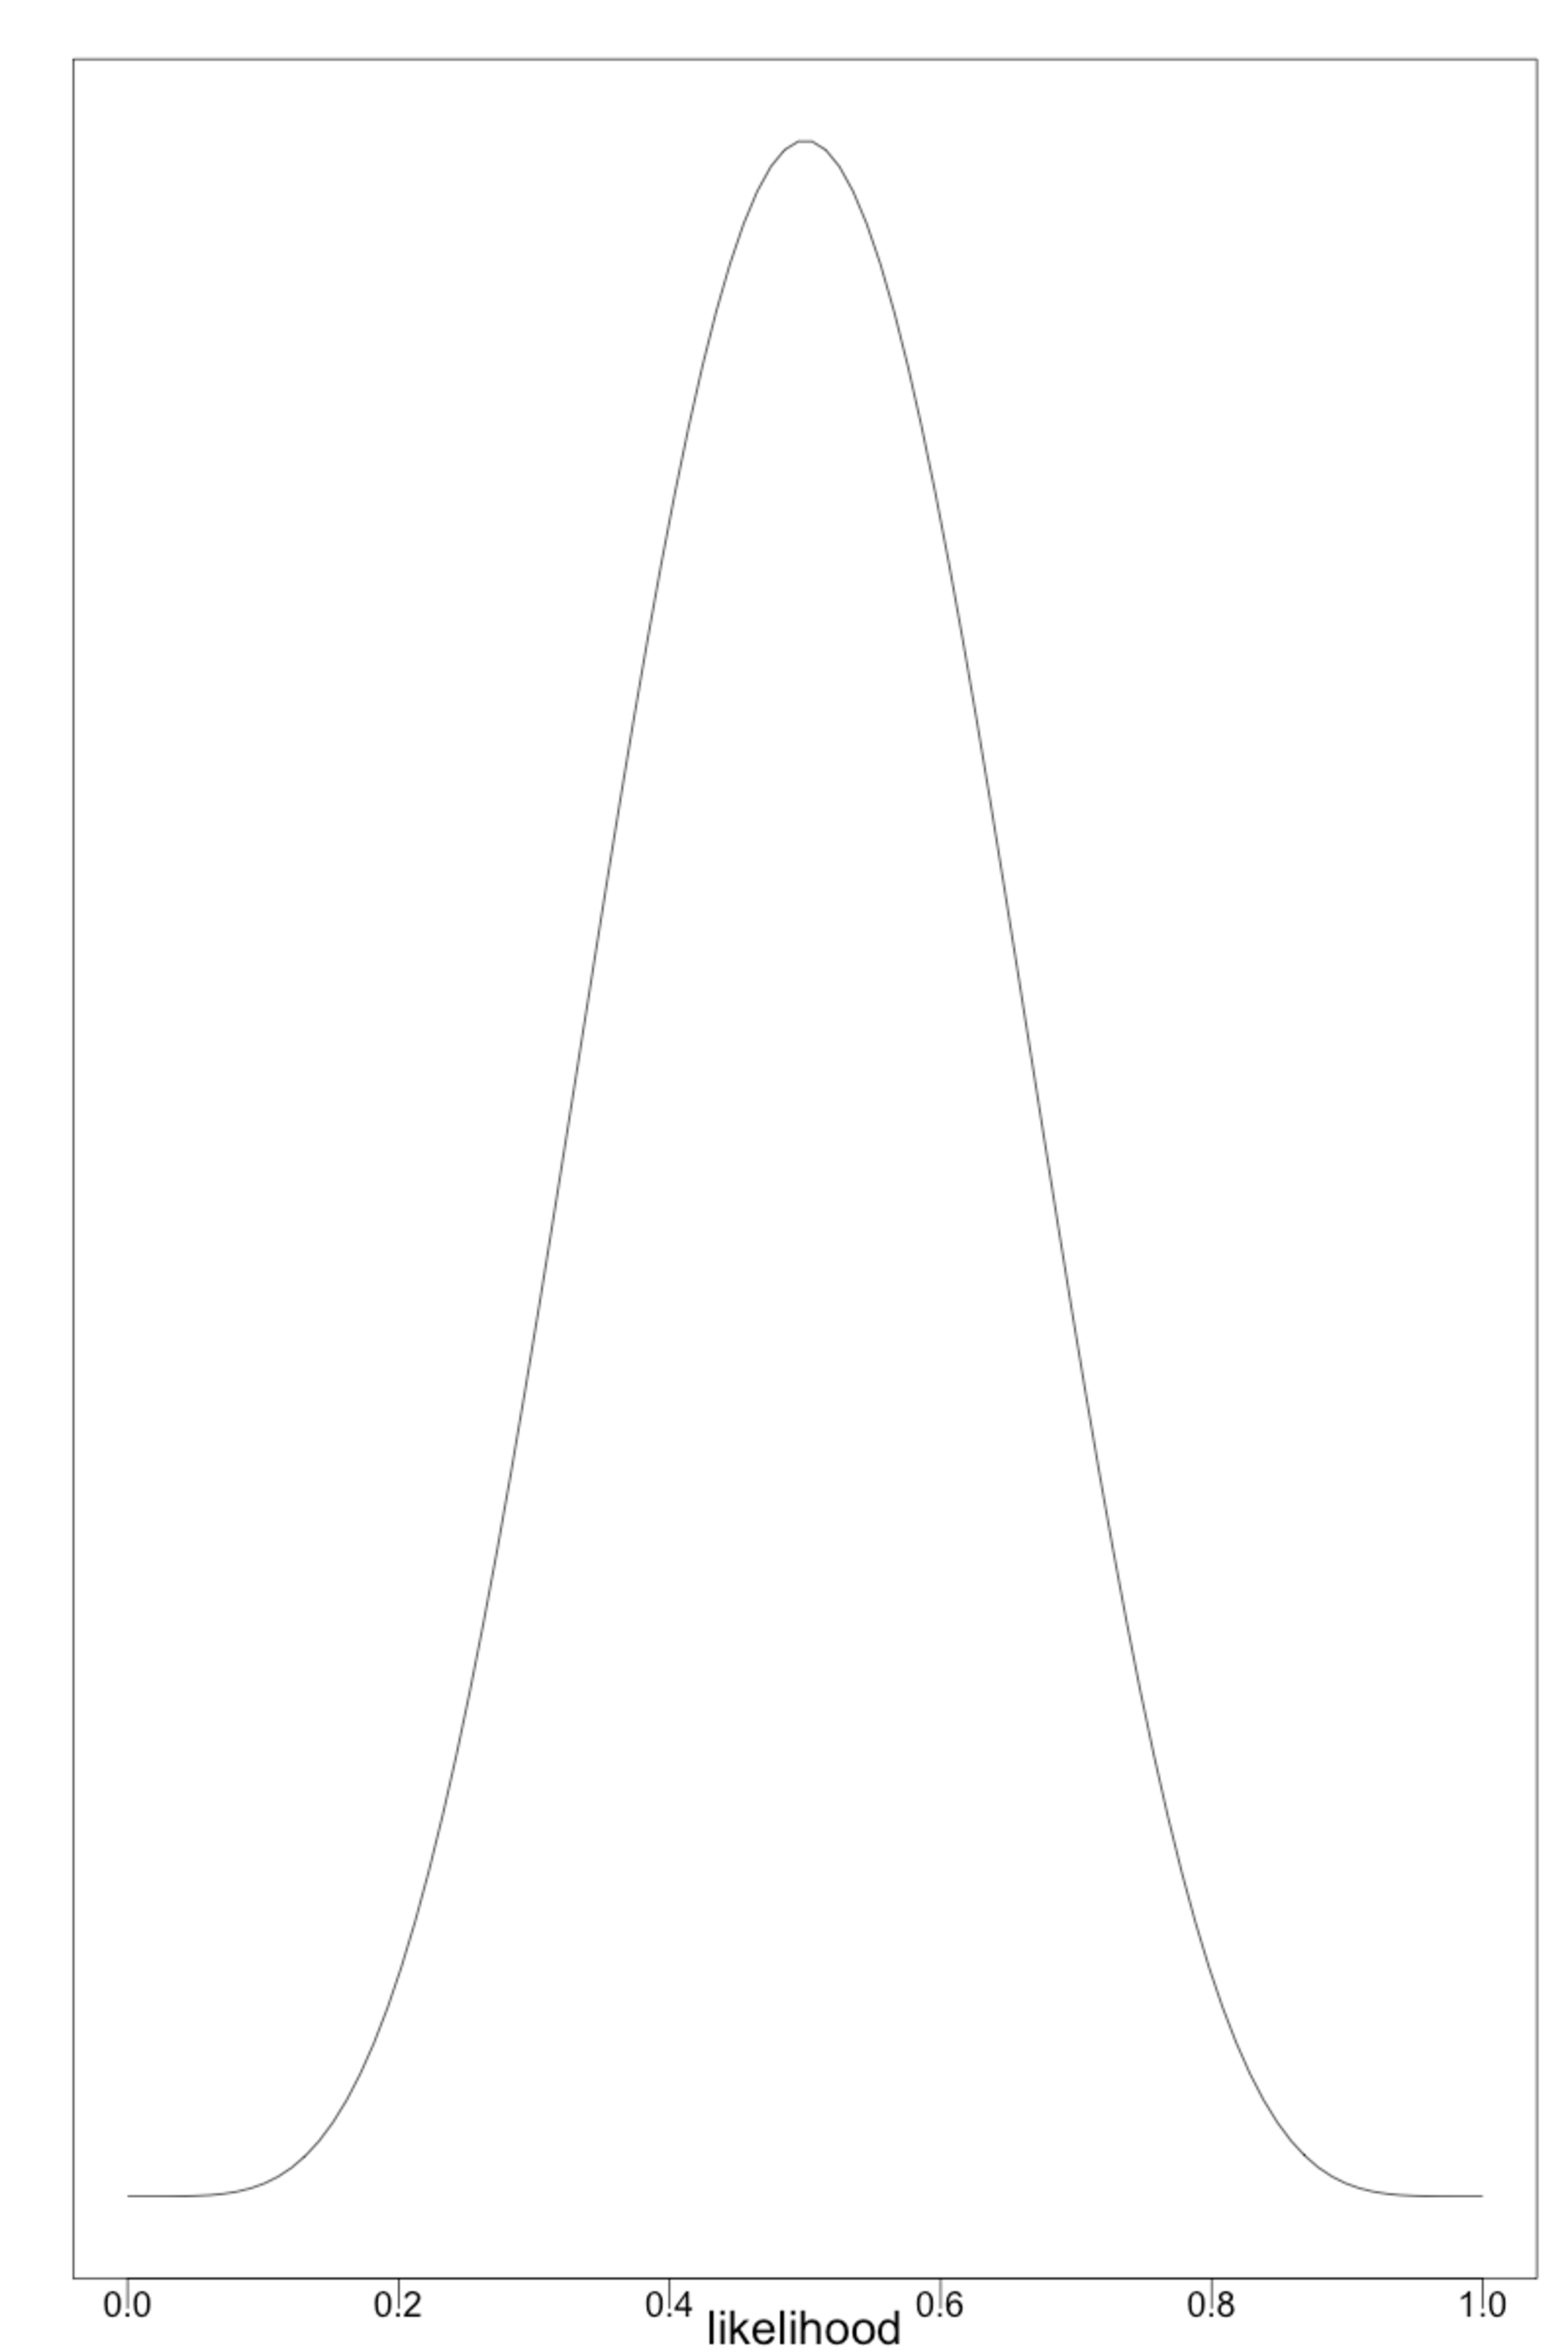
\includegraphics[valign=m, width=100pt]{cointosses/Ten_pre.pdf} $\propto$
%%	    	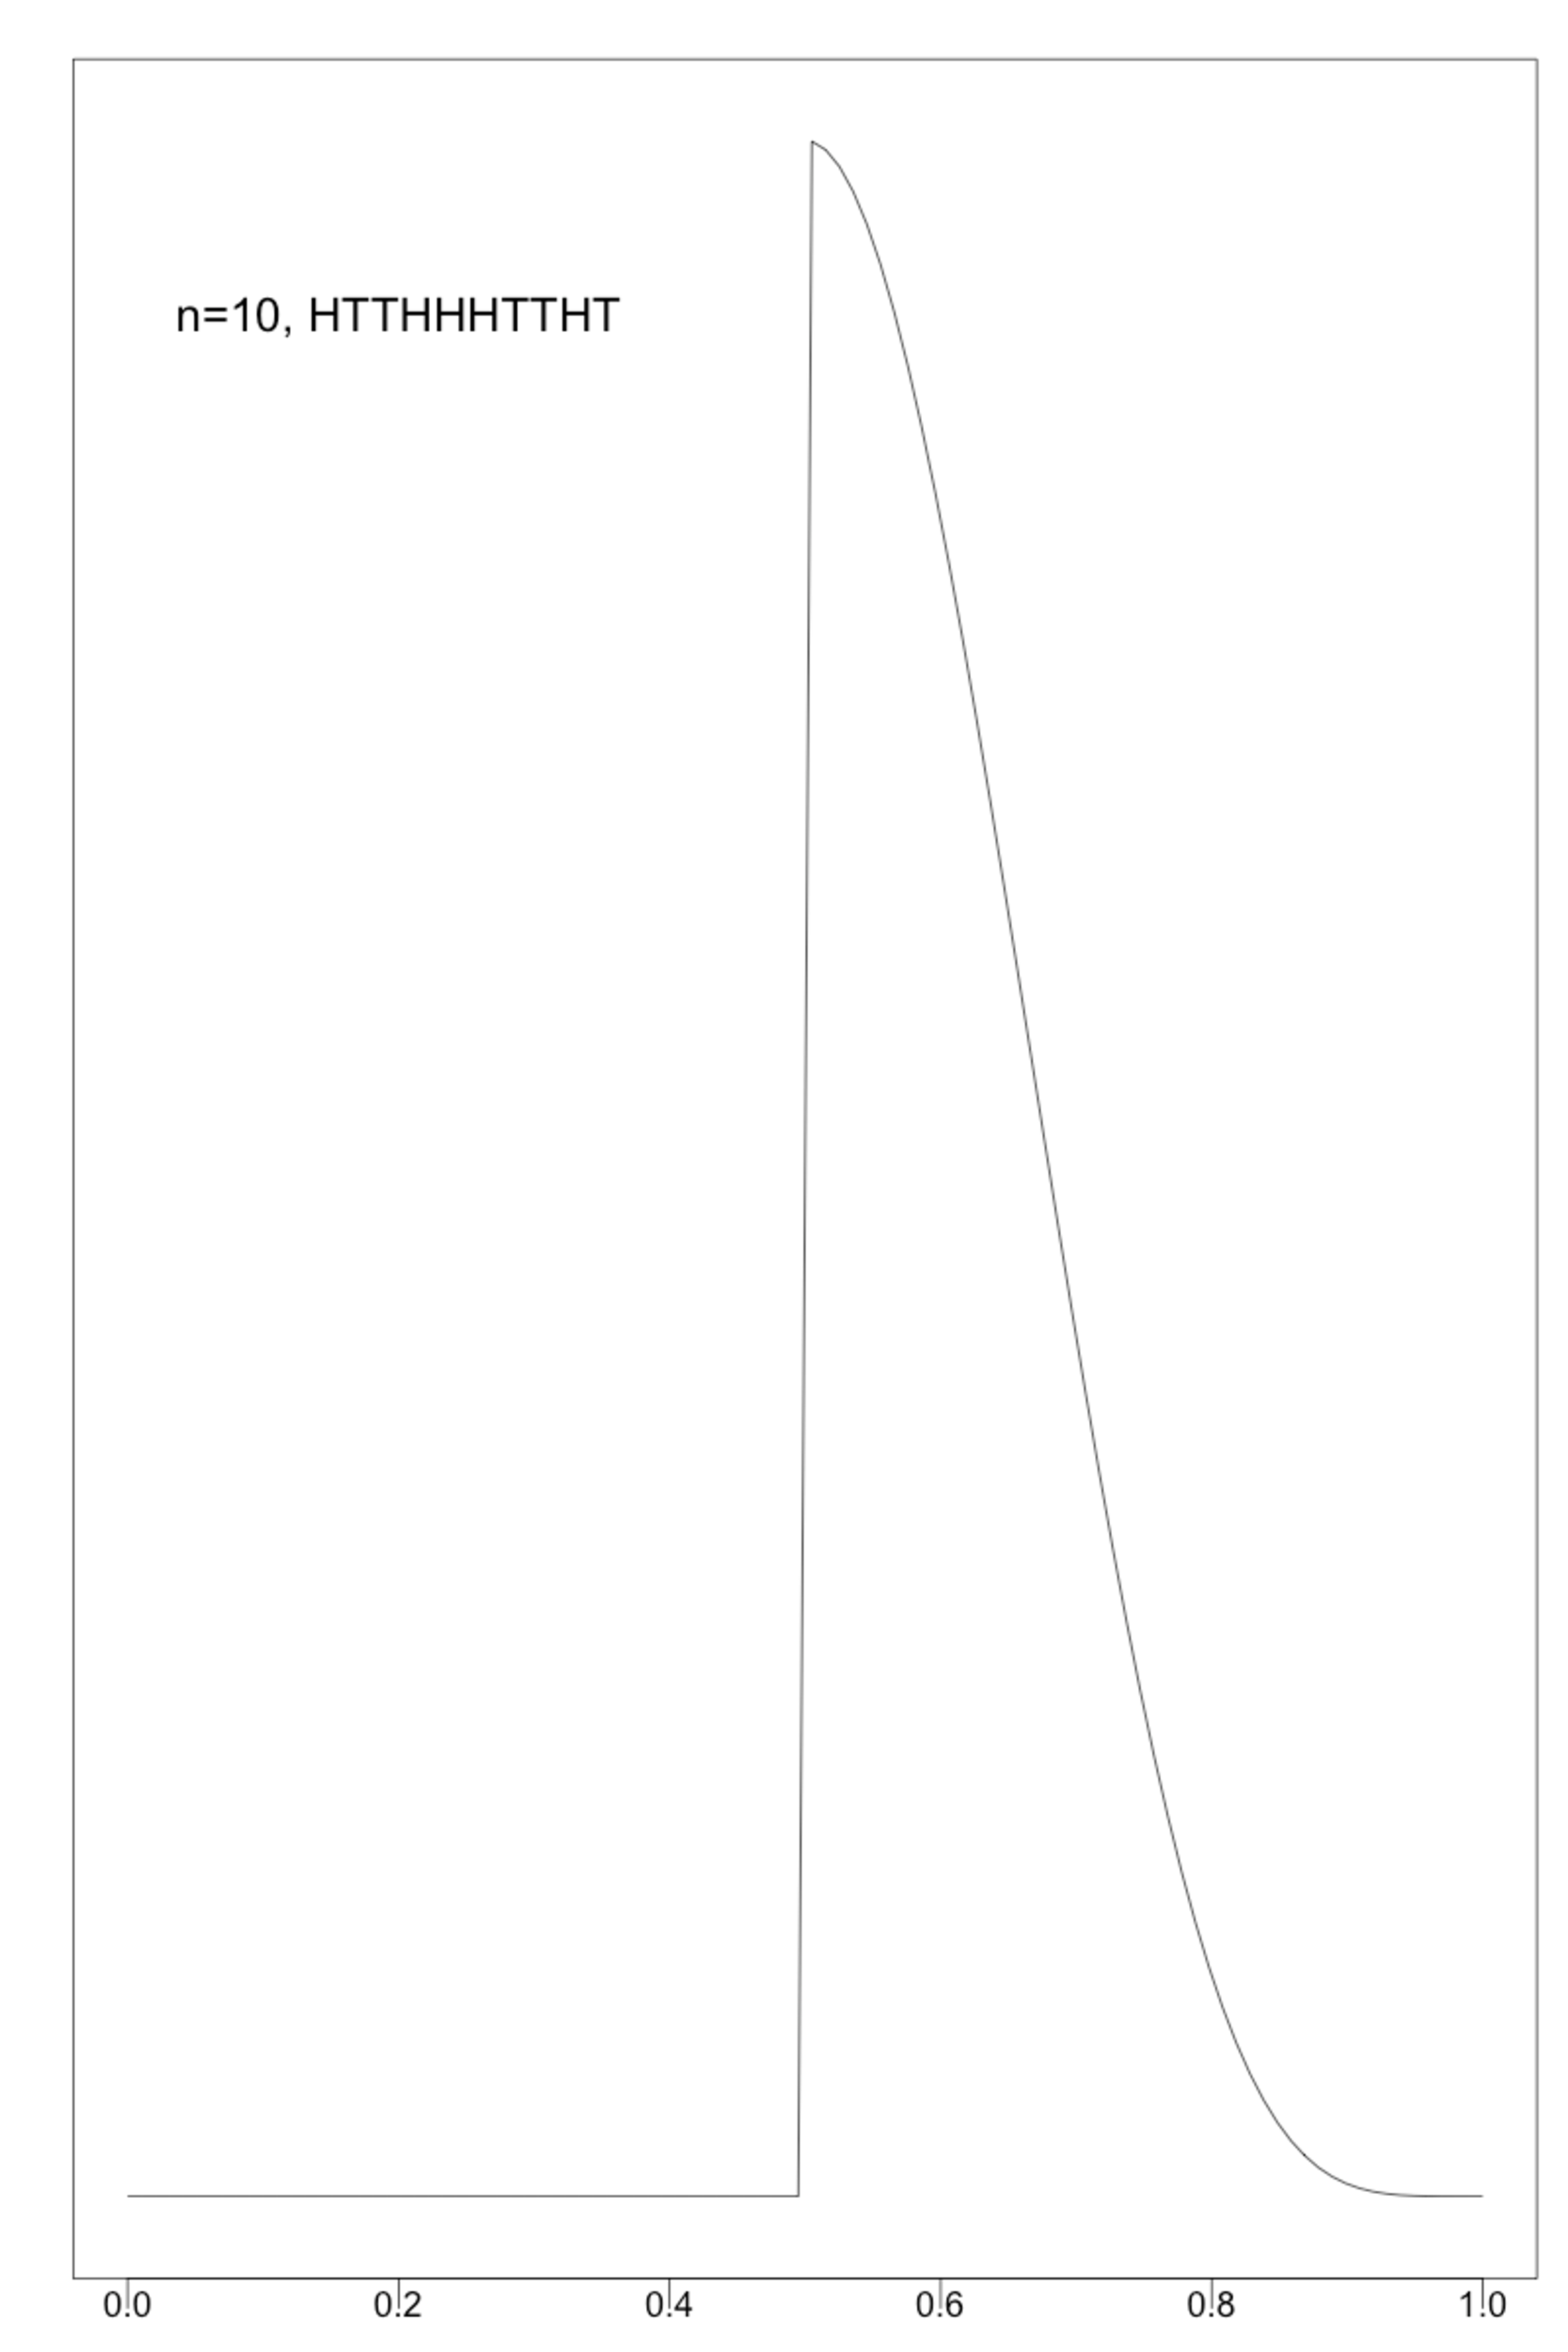
\includegraphics[valign=m, width=100pt]{cointosses/step_Ten.pdf}
%%\end{frame}
%%
%%\begin{frame}{Ten Coin Tosses}{Some Other Priors}
%%		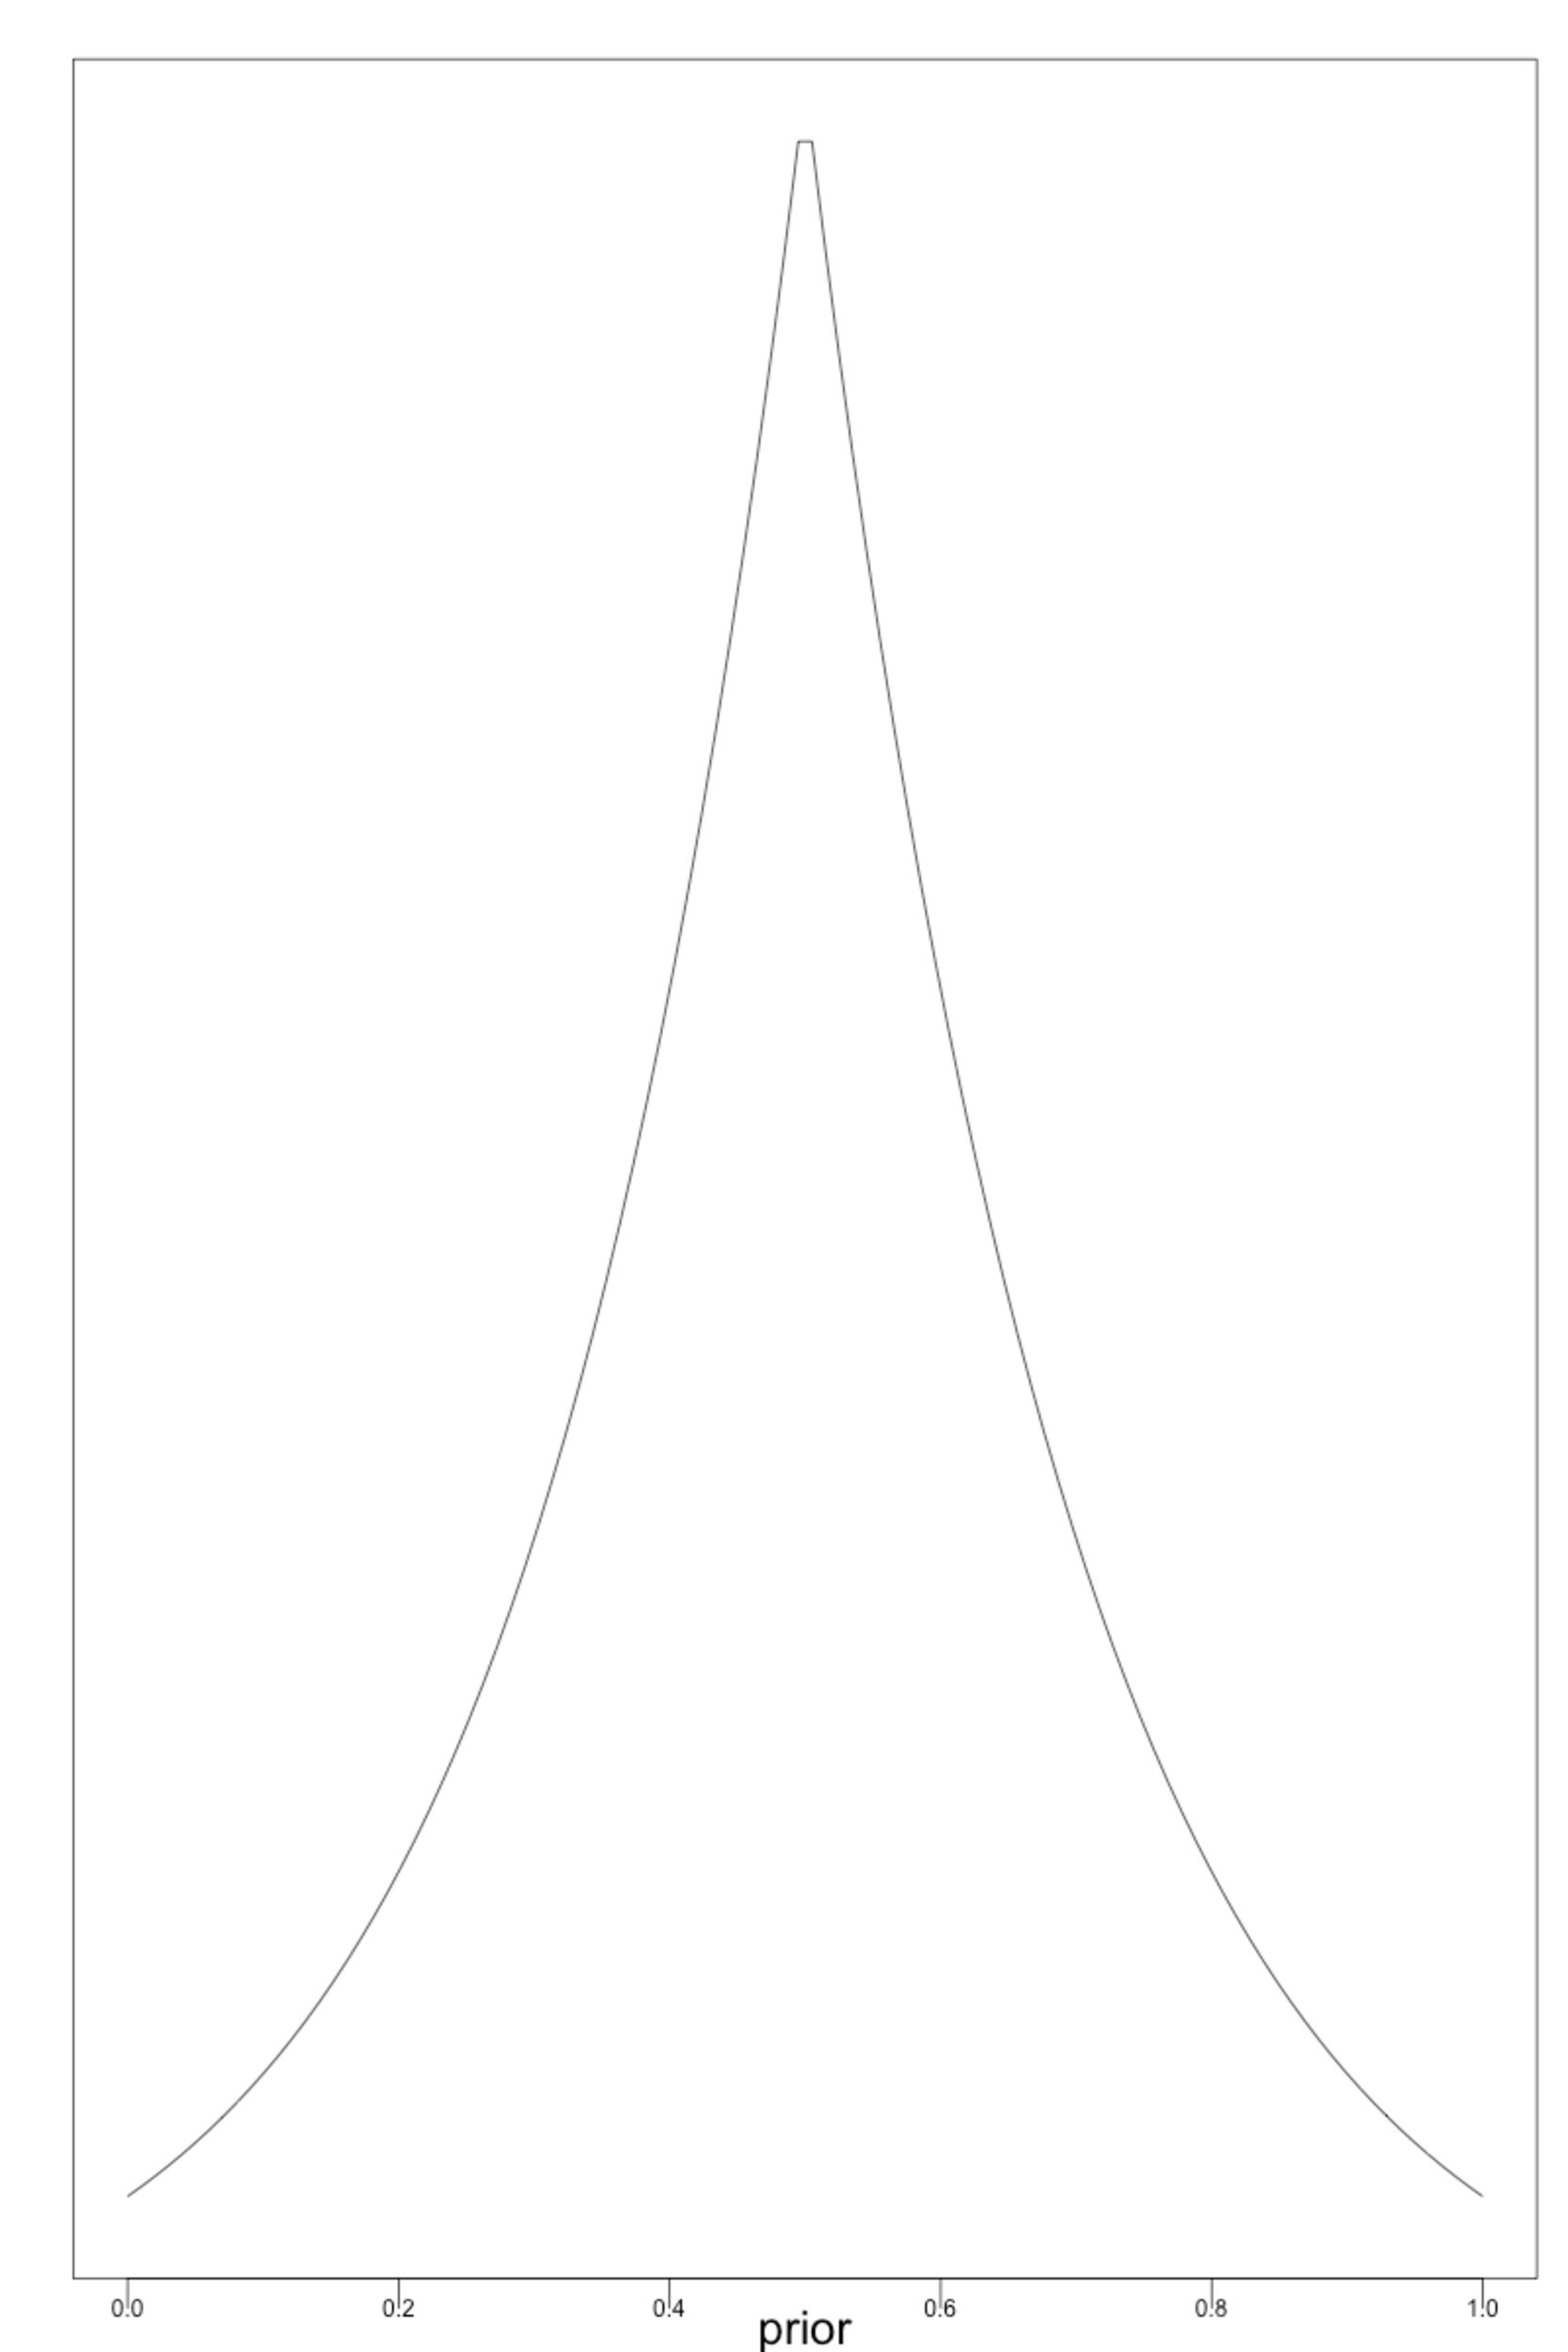
\includegraphics[valign=m, width=100pt]{cointosses/peaked_prior.pdf} $\times$
%%	    	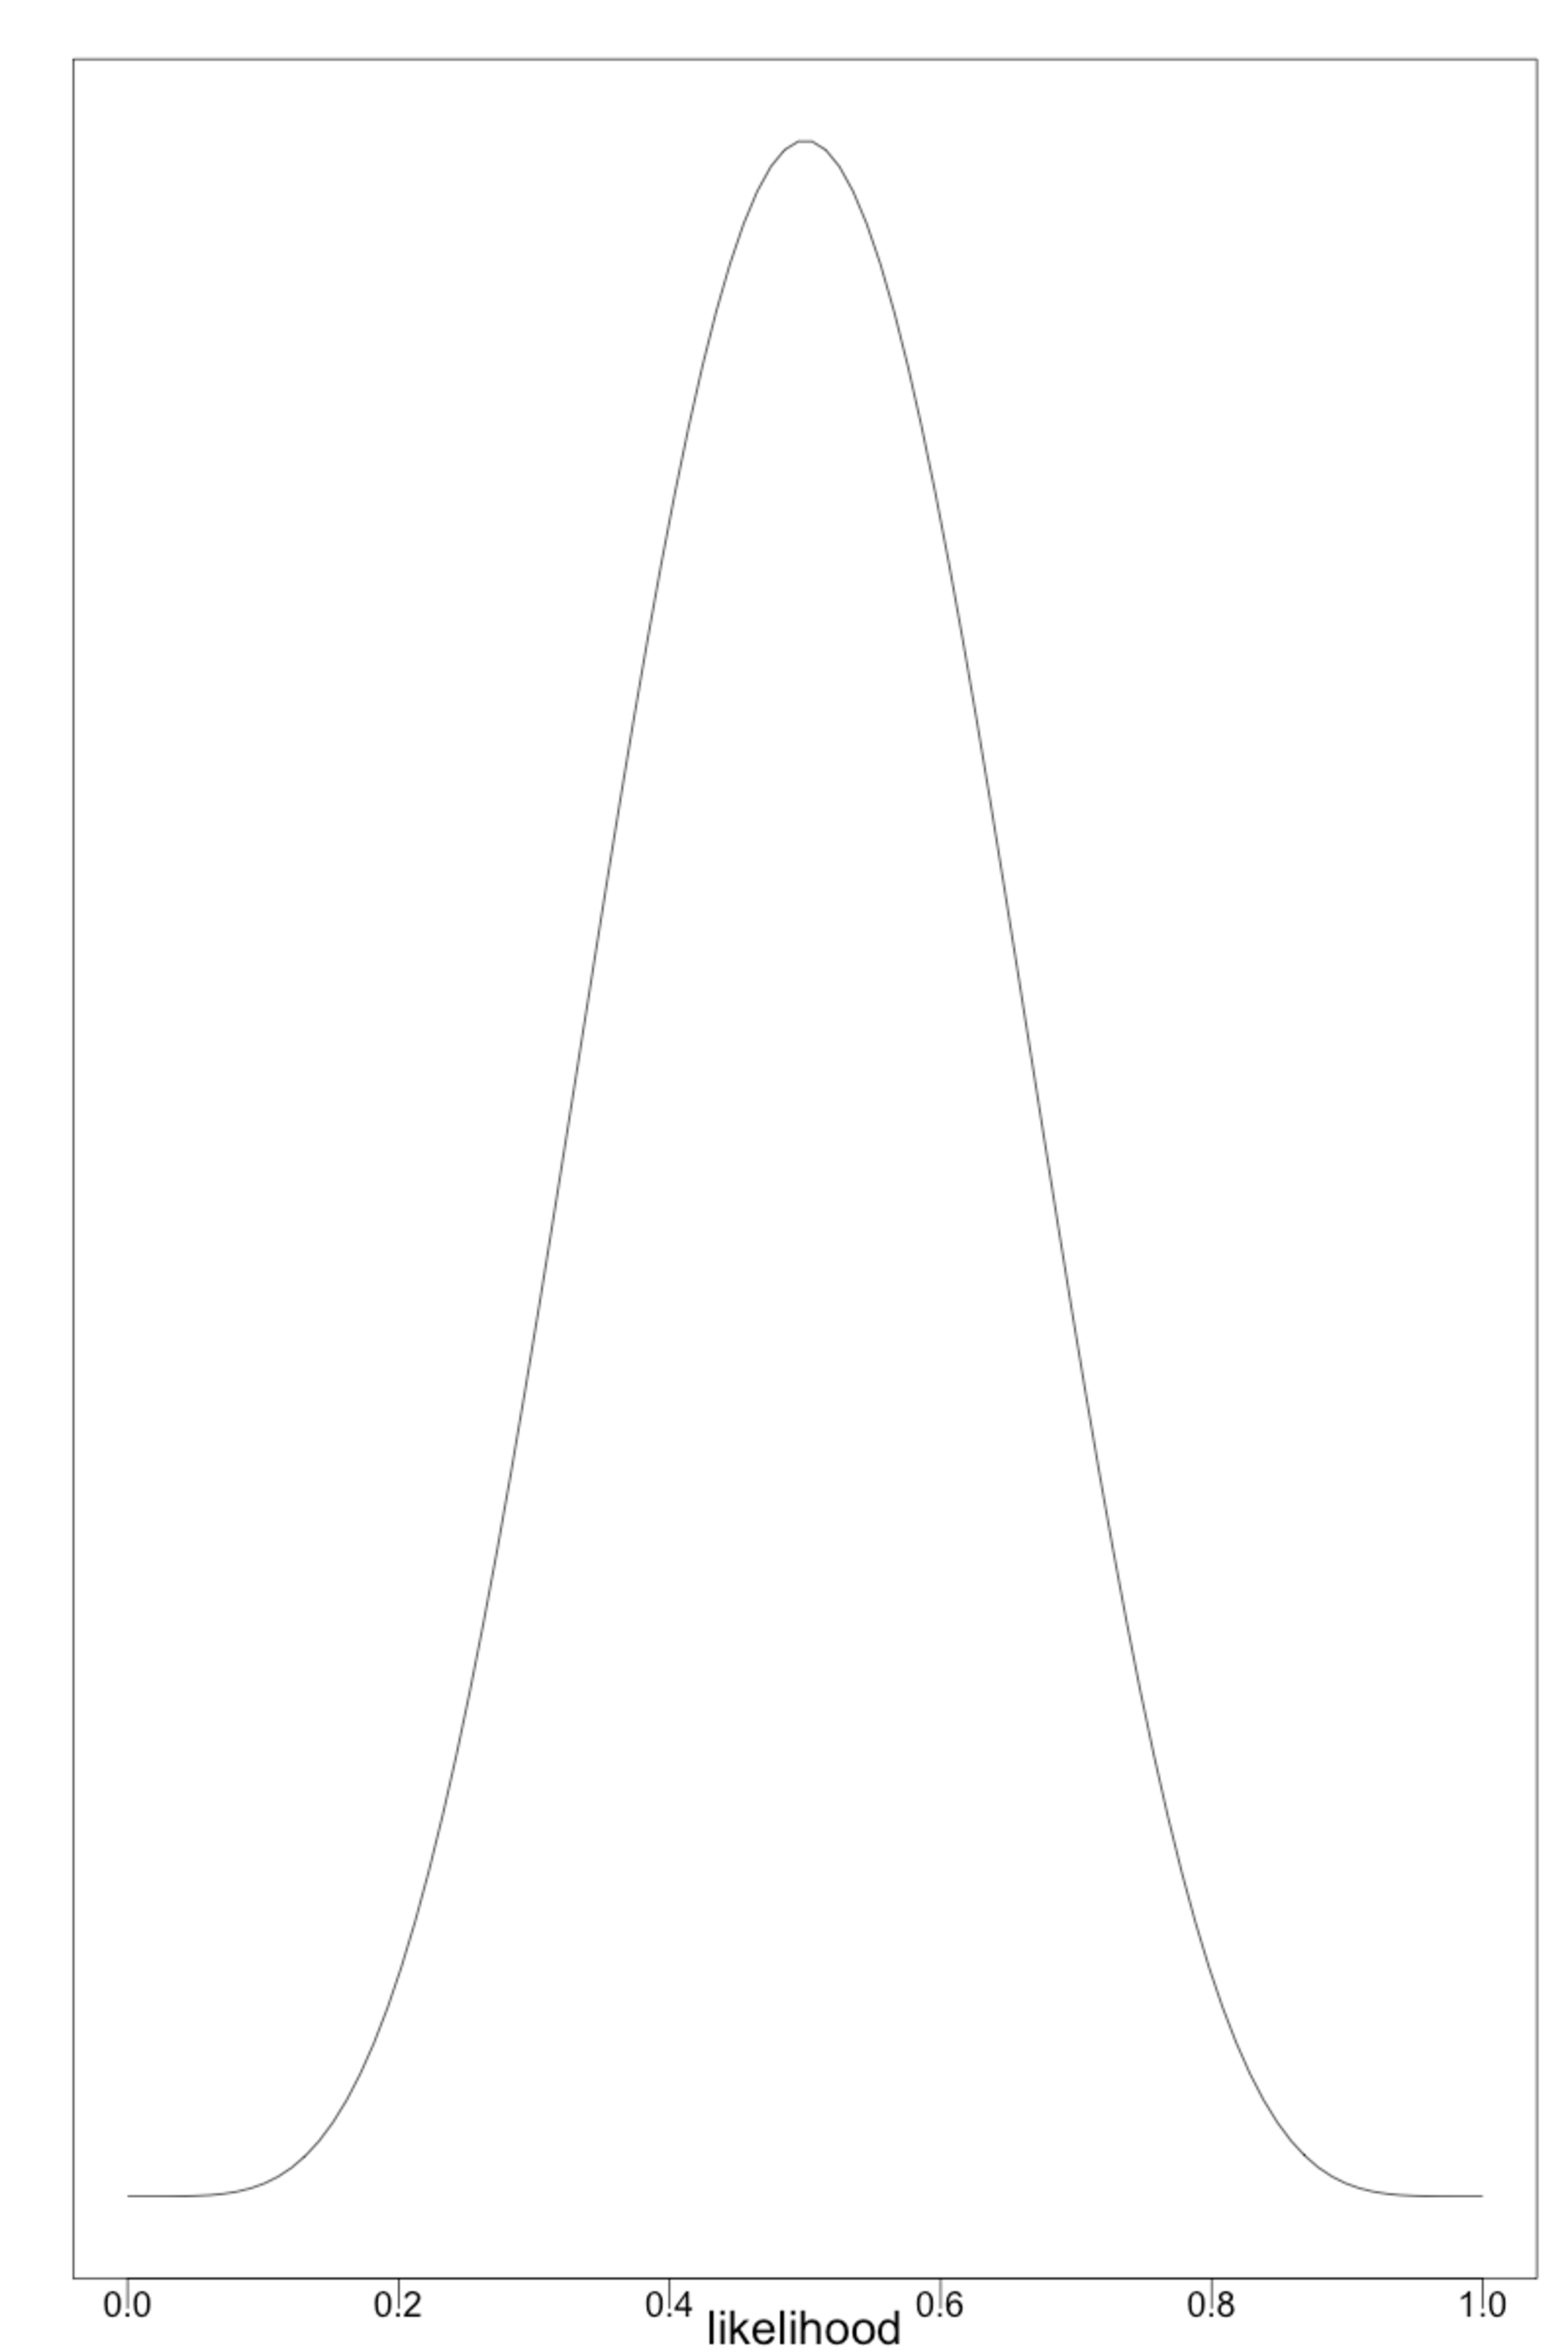
\includegraphics[valign=m, width=100pt]{cointosses/Ten_pre.pdf} $\propto$
%%	    	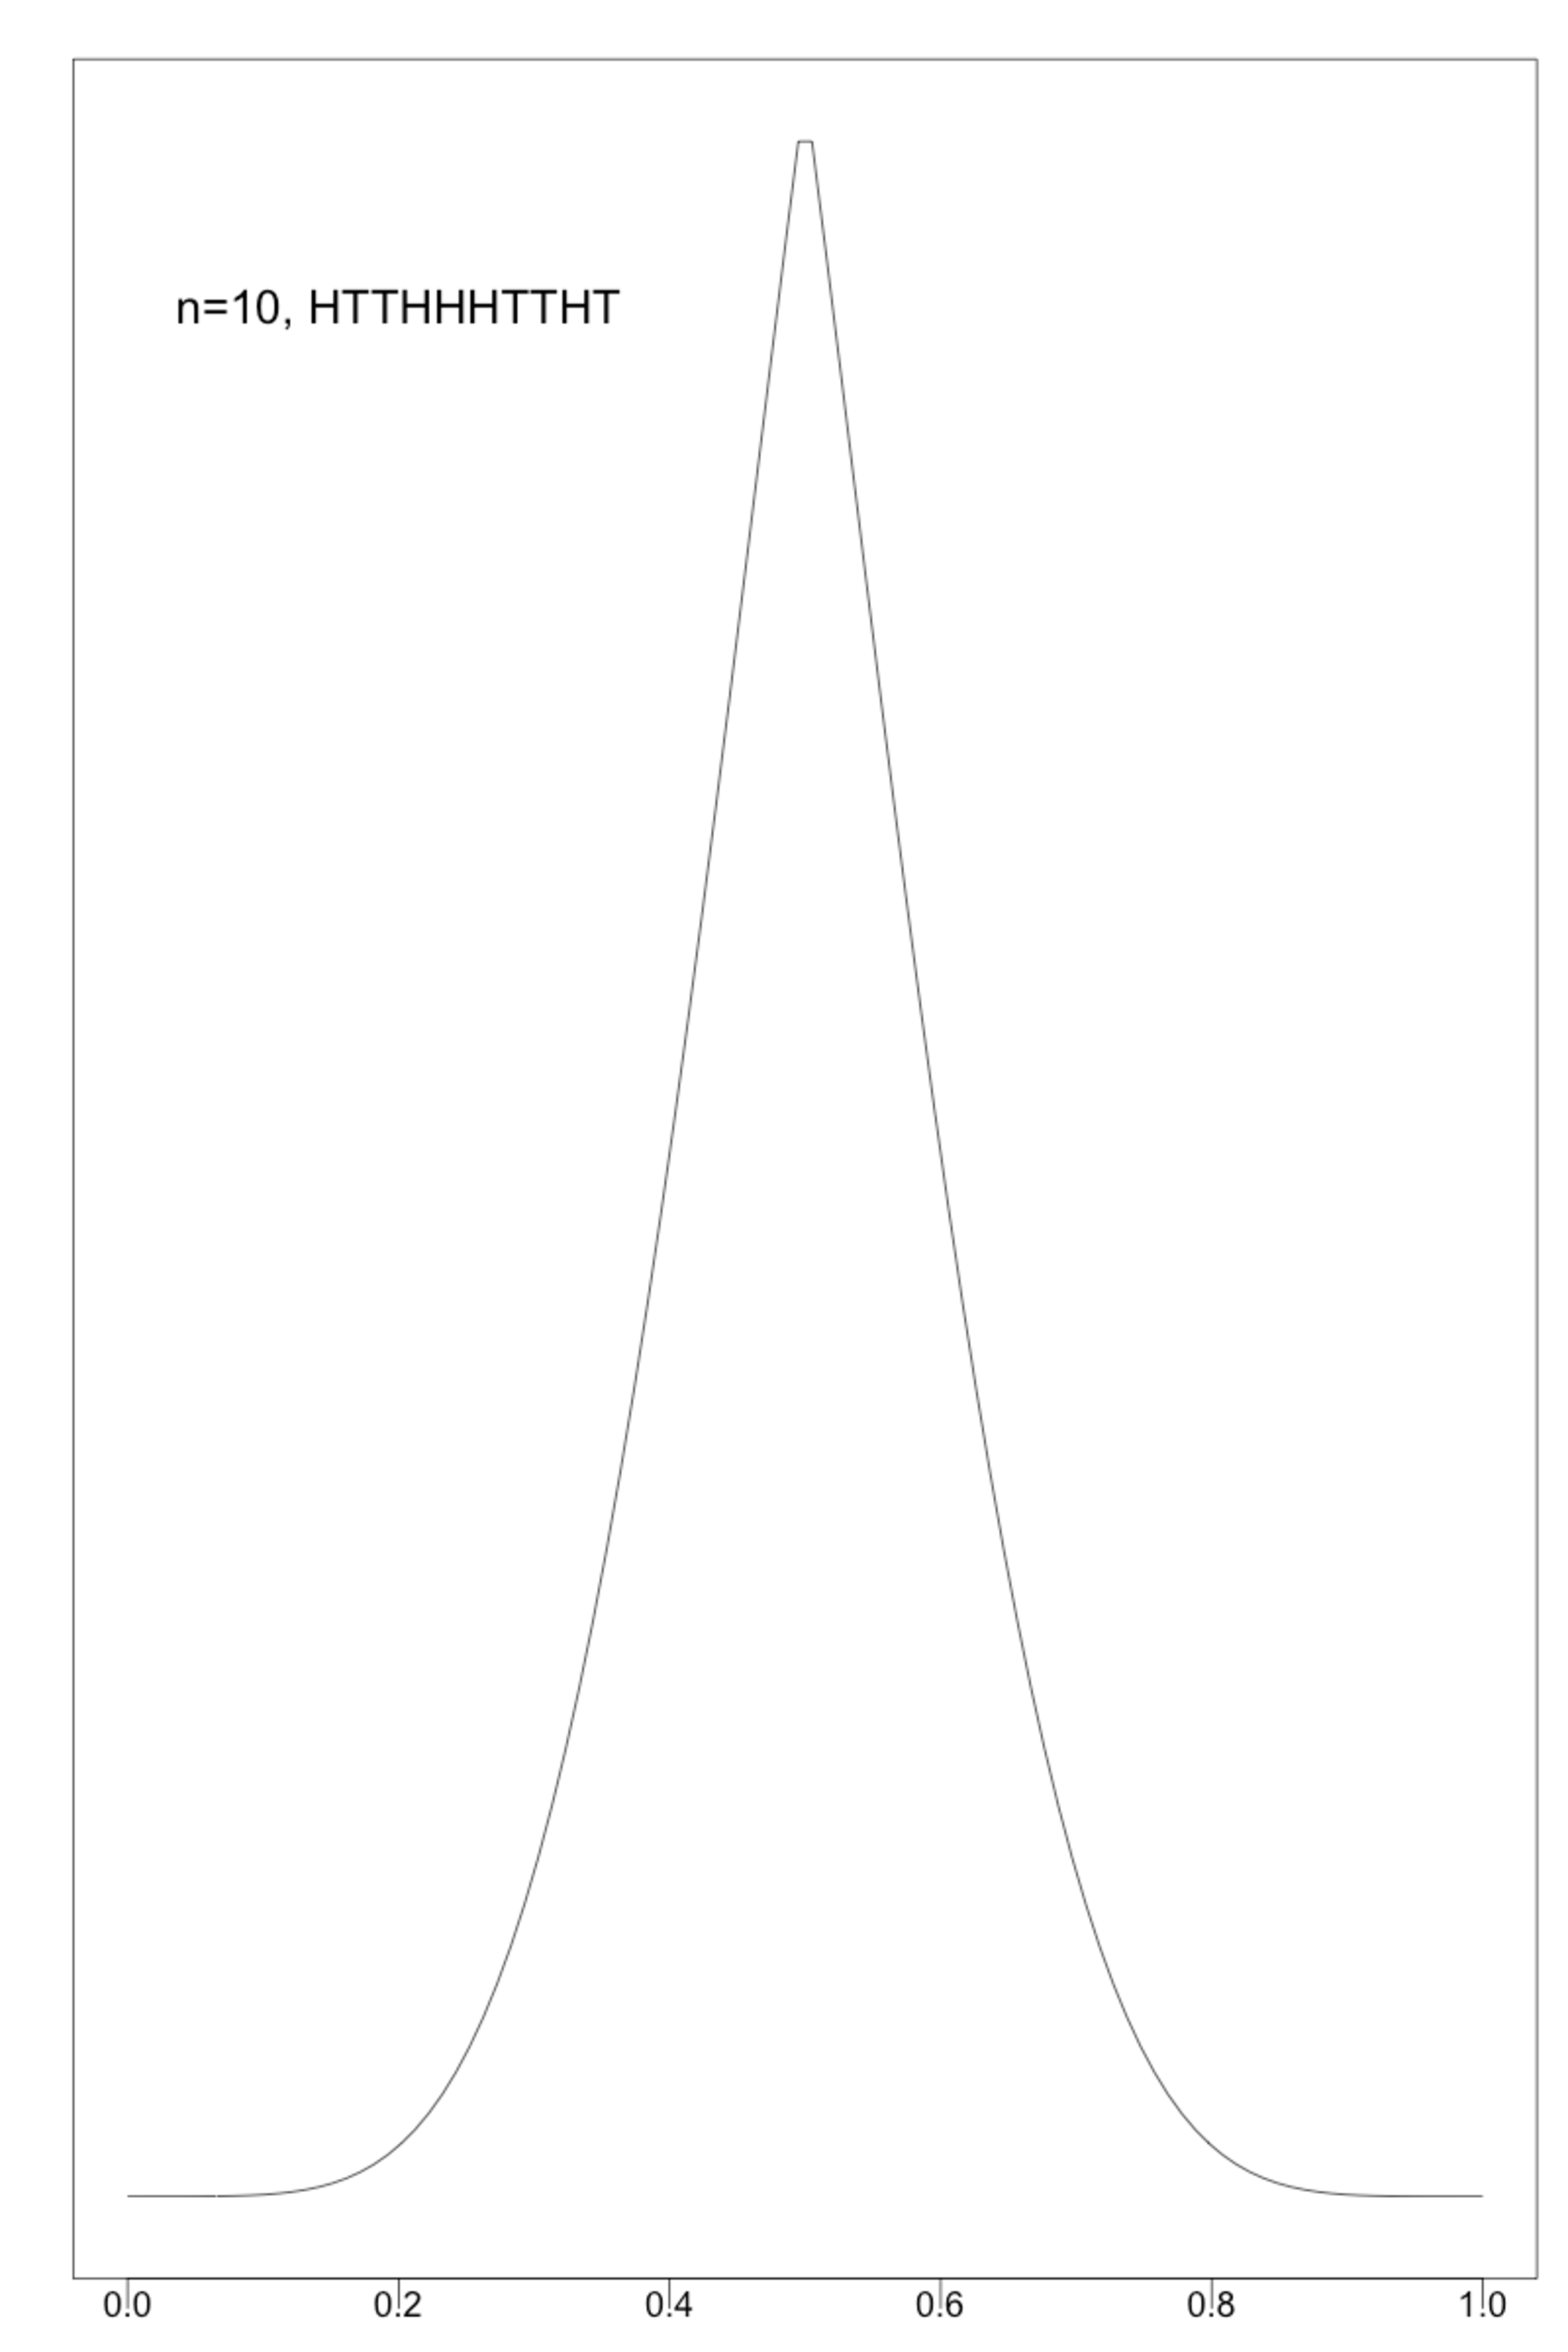
\includegraphics[valign=m, width=100pt]{cointosses/peaked_Ten.pdf}
%%\end{frame}
%%
%%\begin{frame}{Ten Coin Tosses}{Sampling From Posterior}
%%	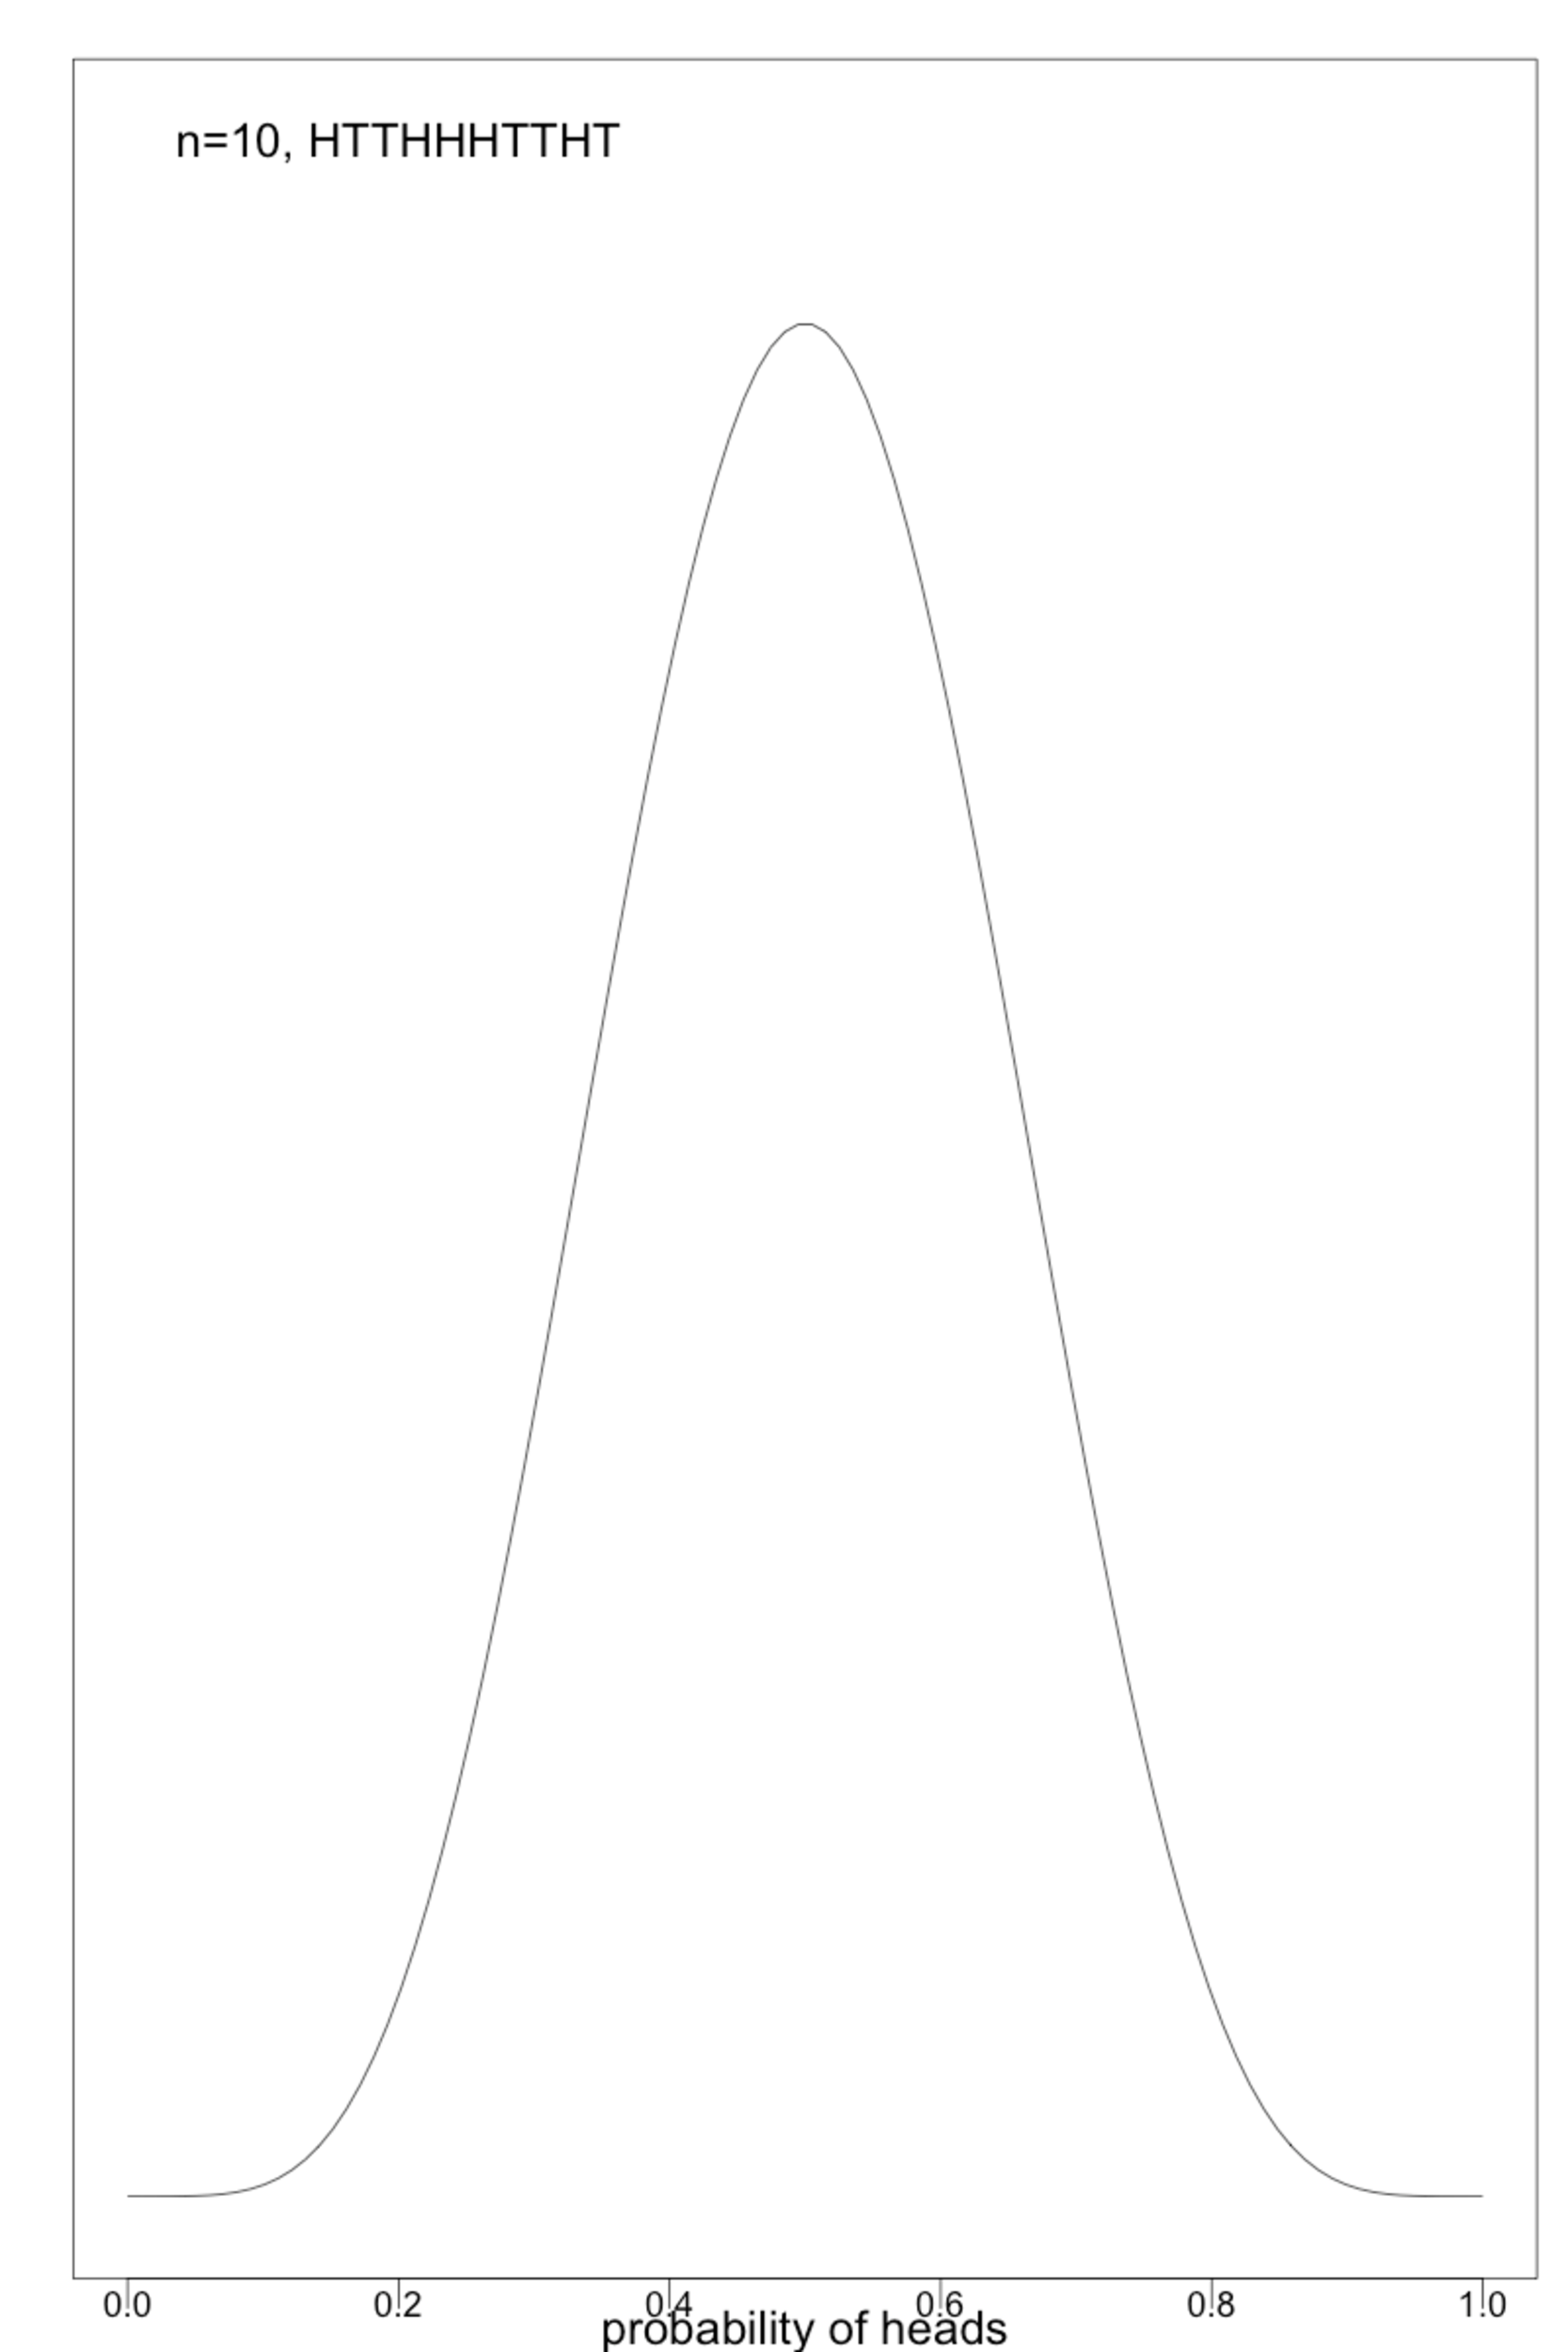
\includegraphics[valign=m, width=100pt]{cointosses/Ten.pdf} $\longrightarrow$
%%    	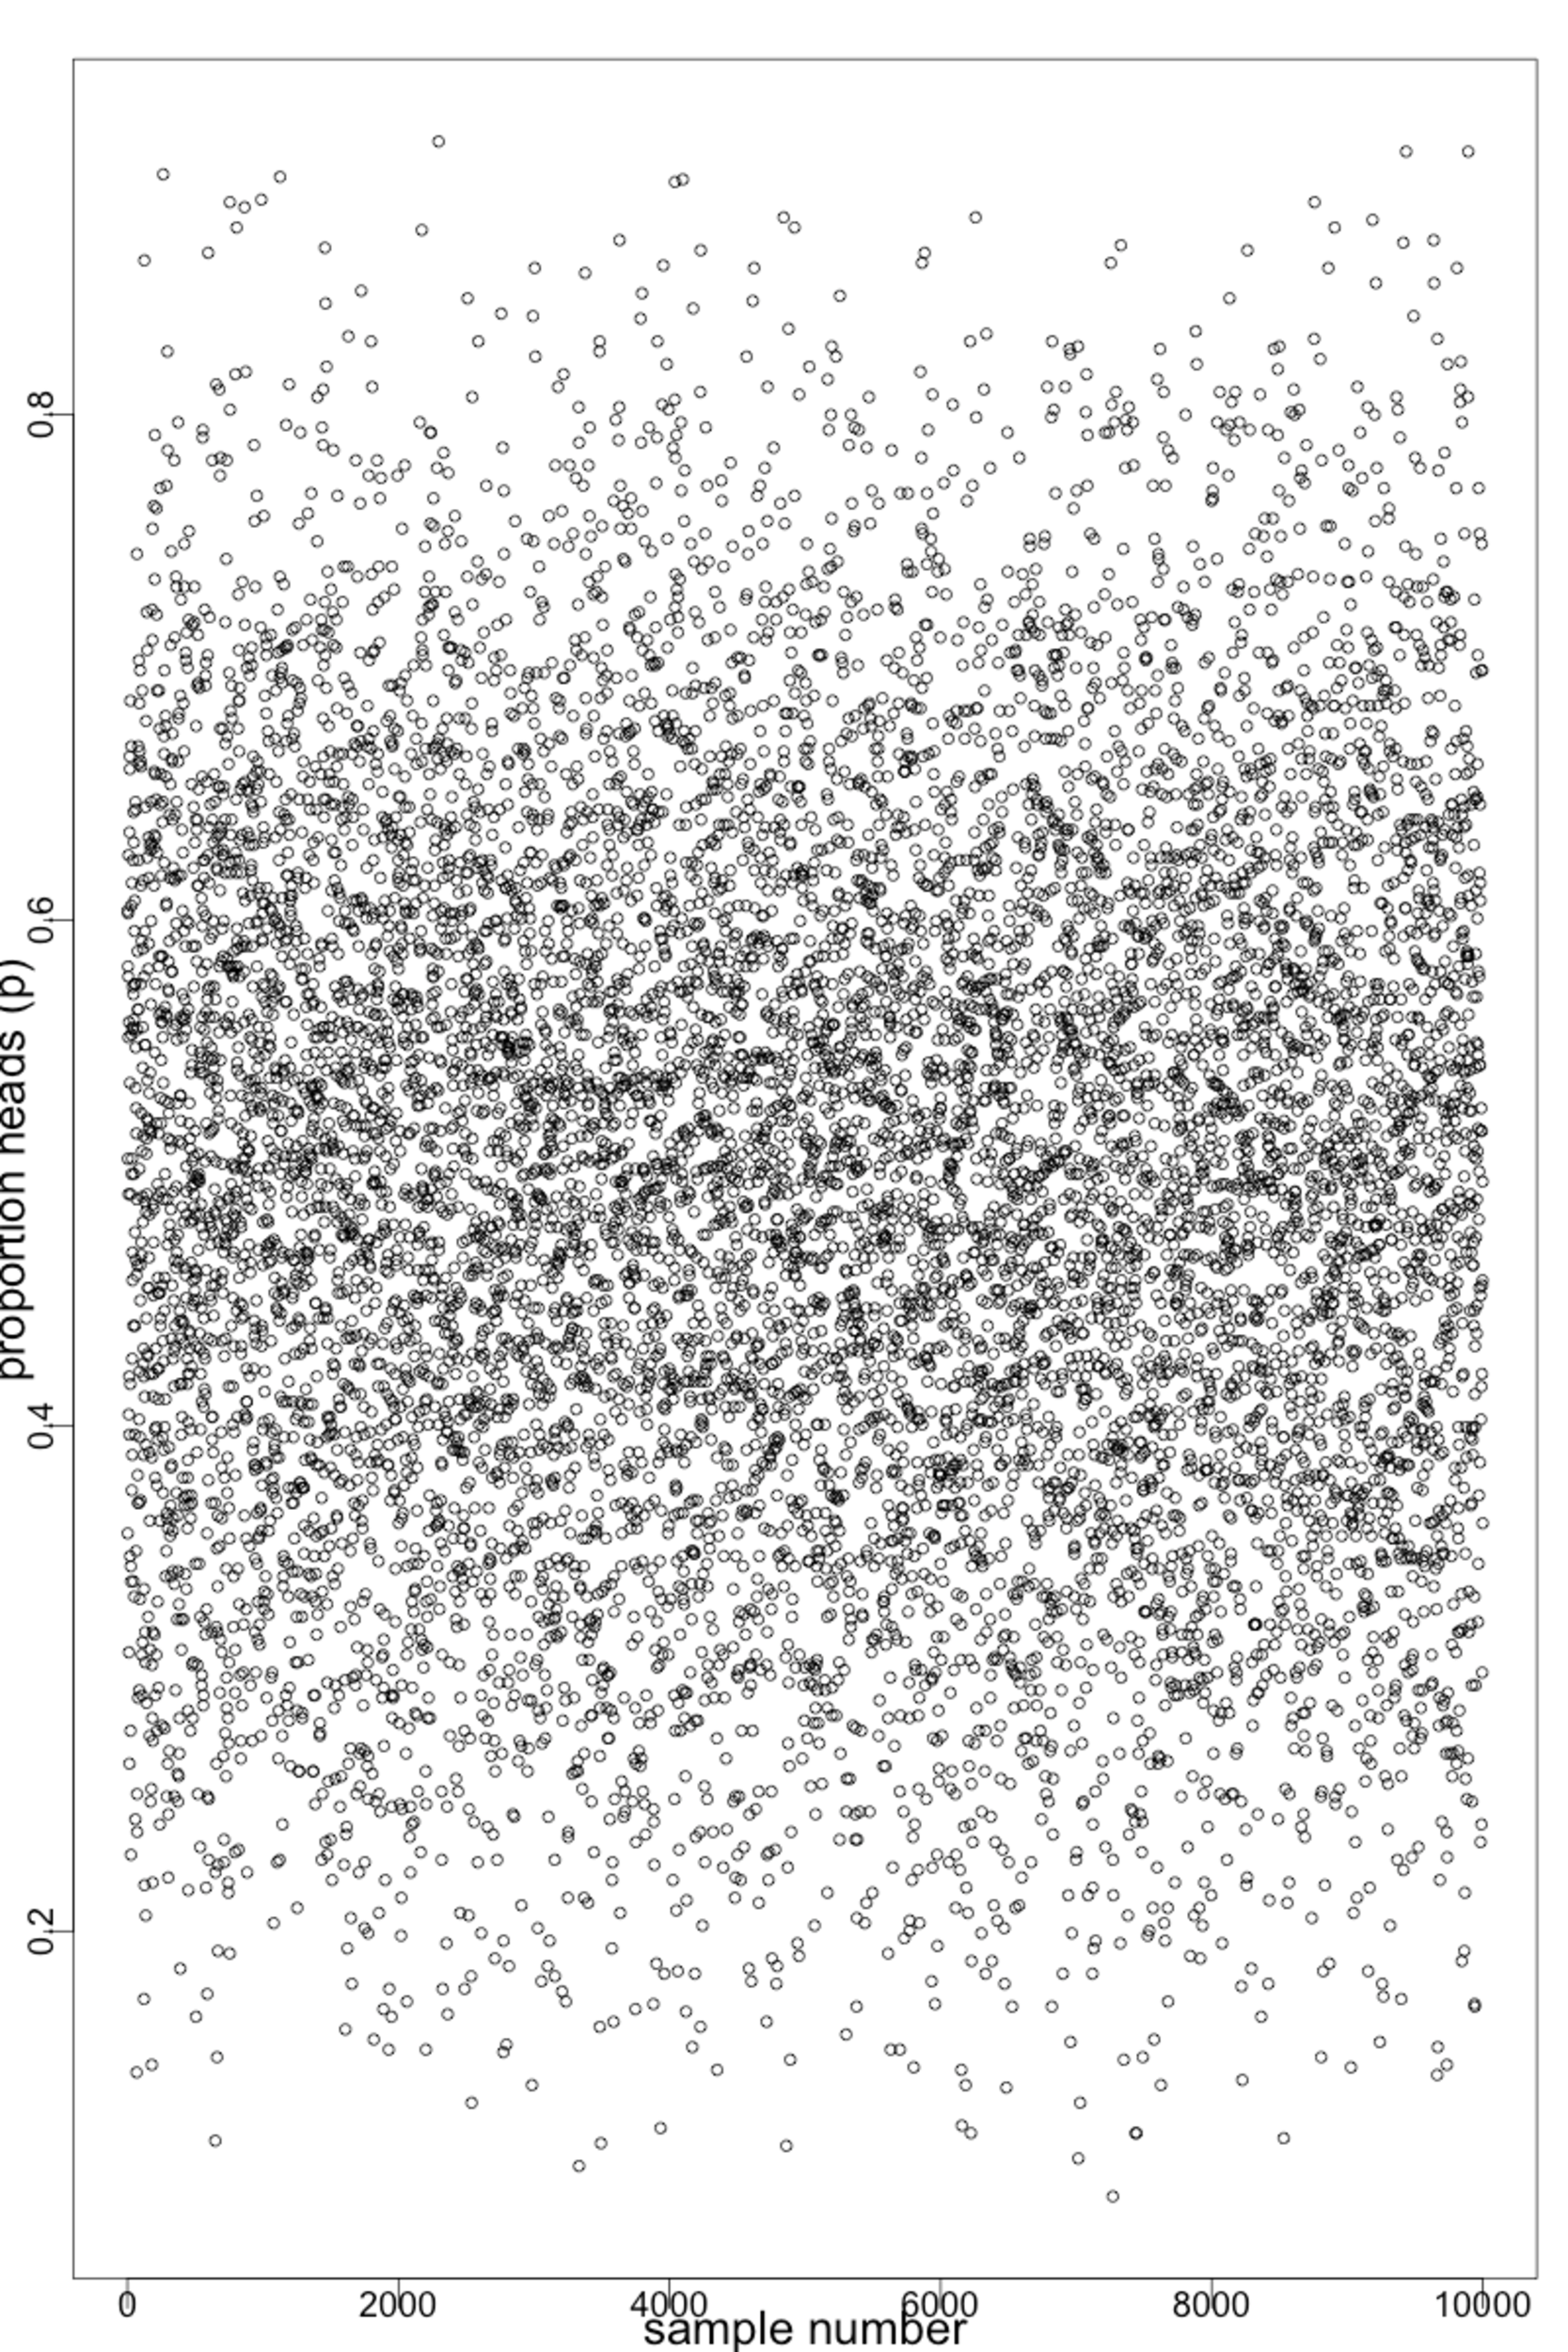
\includegraphics[valign=m, width=100pt]{cointosses/samples.pdf} $\longrightarrow$
%%    	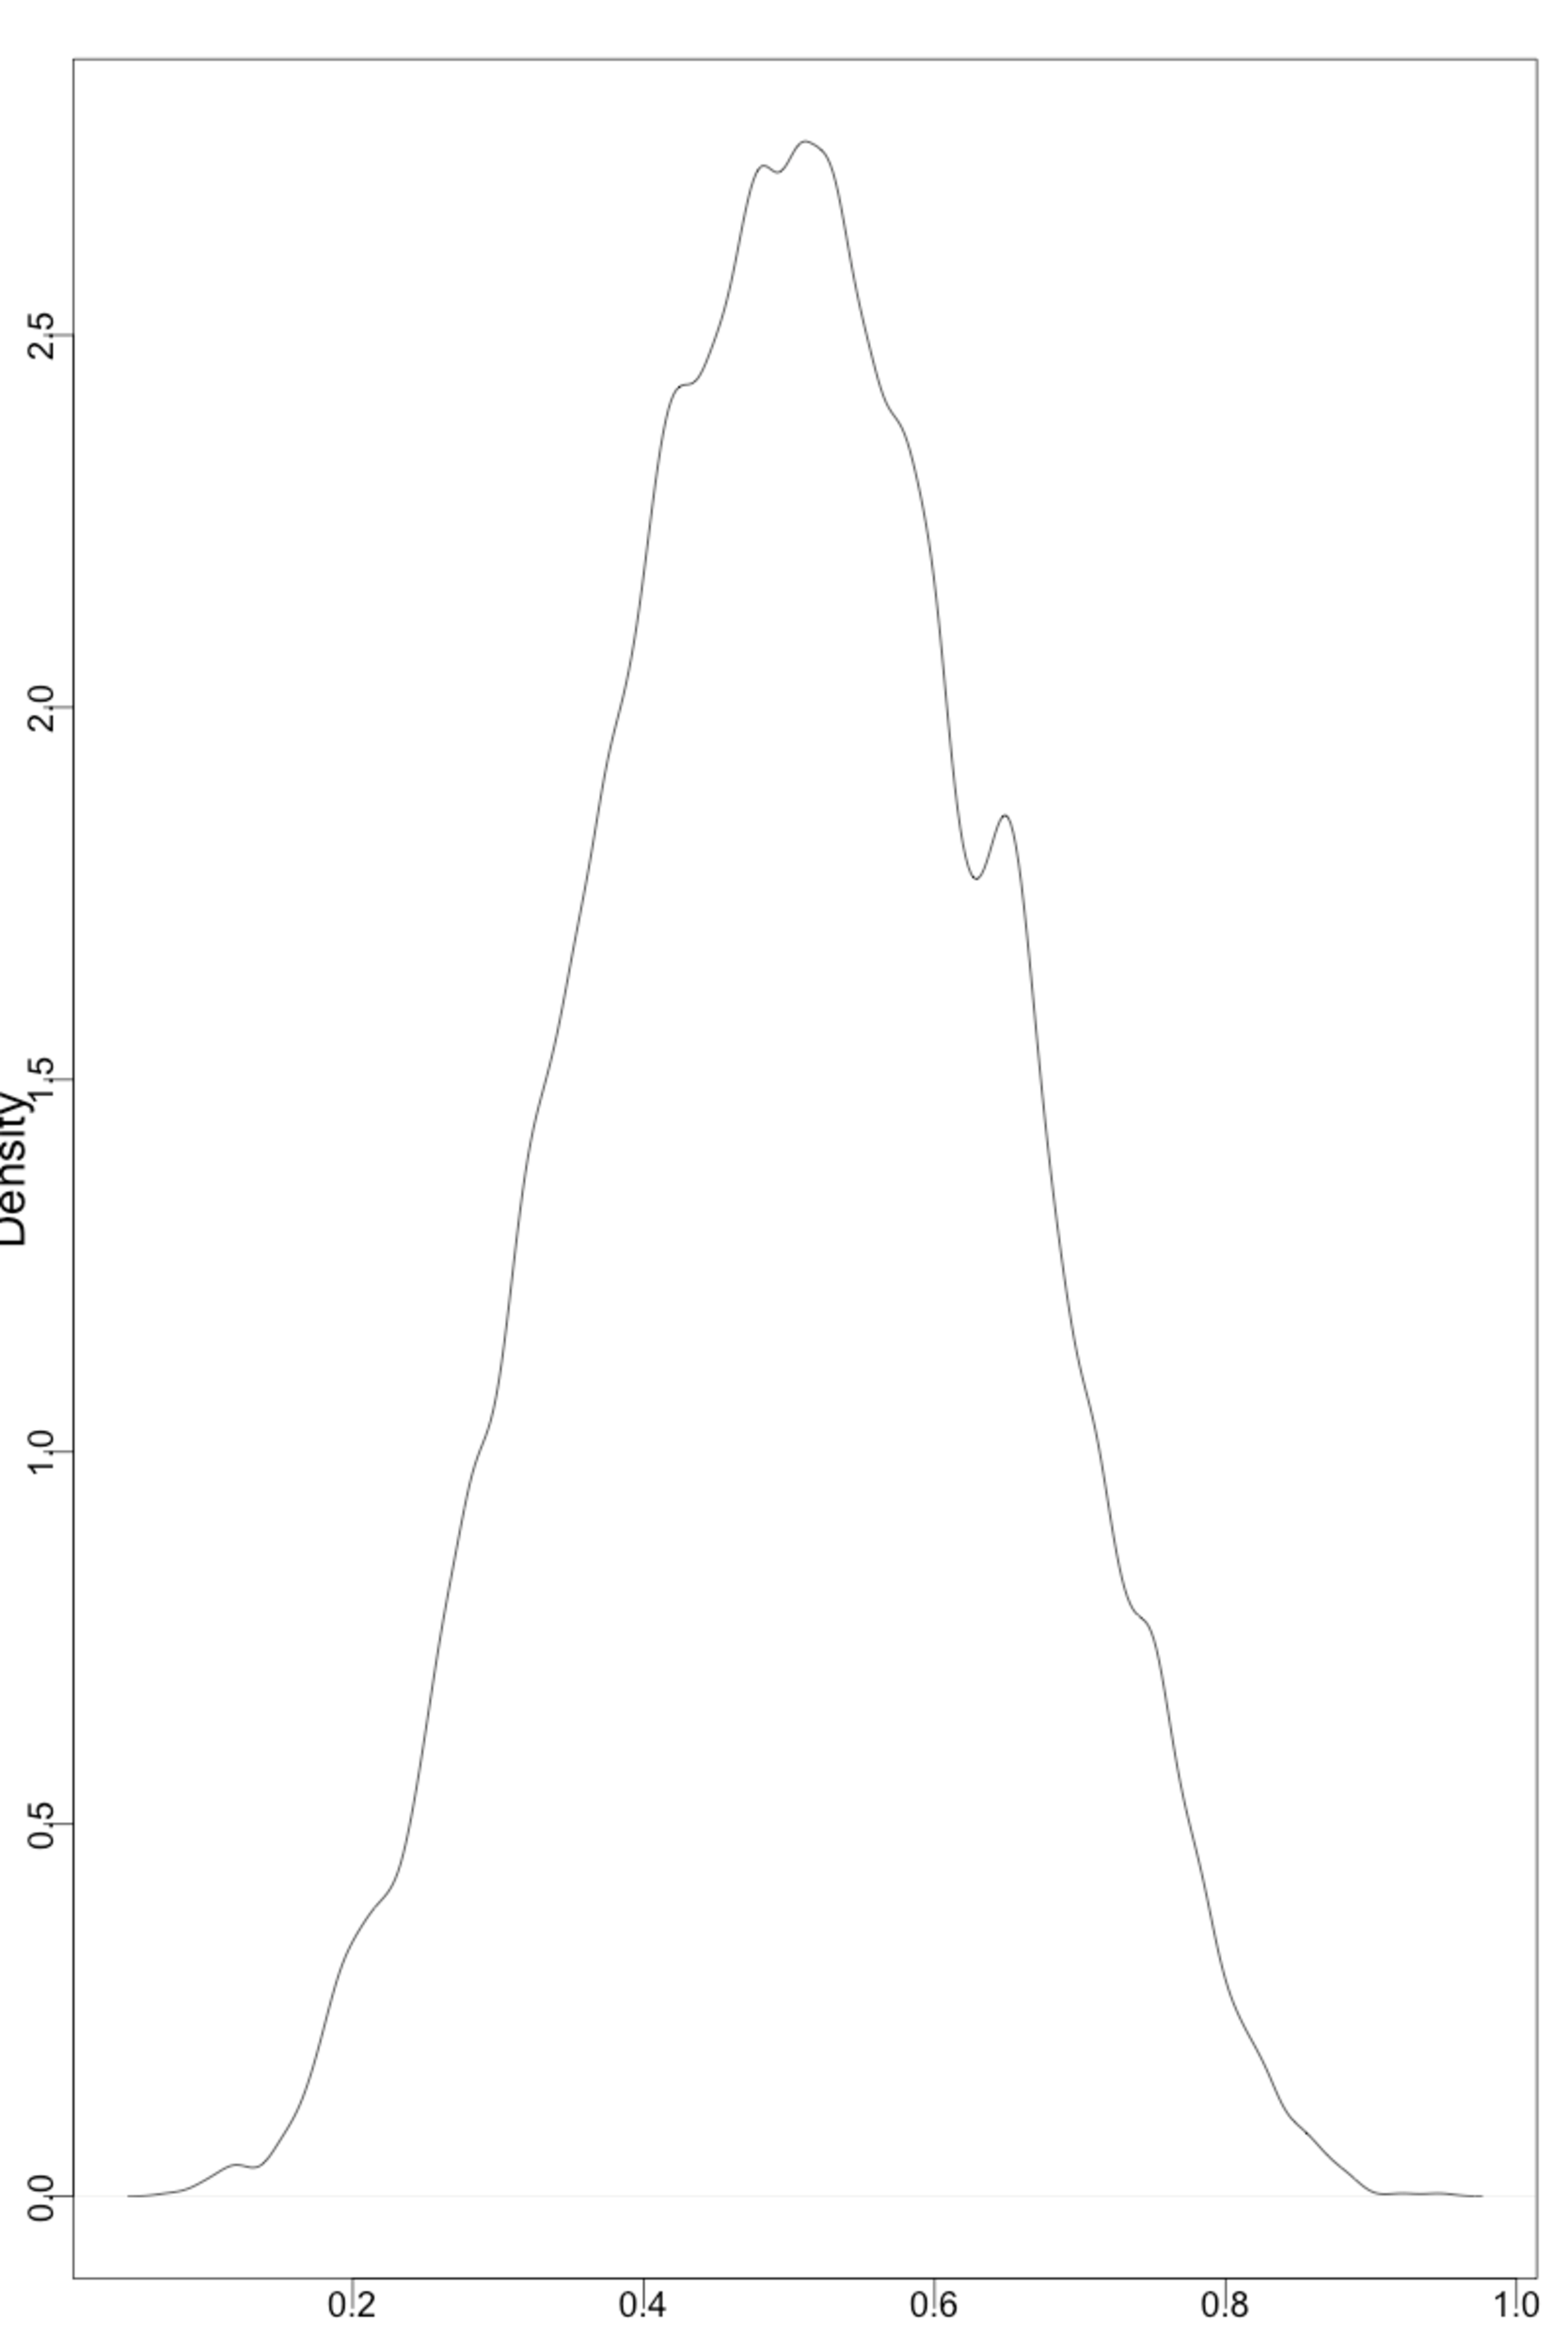
\includegraphics[valign=m, width=100pt]{cointosses/sample_density.pdf}
%%\end{frame}
%	
%
%%\section{Marbles}
%%
%%\begin{frame}
%%    \begin{itemize}
%%    	\item There's a bag that contains four marbles. \pause
%%    	\item The marbles come in two colors: blue and white. \pause
%%    	\item We know there are four marbles in the bag. \pause
%%    	\item We don't know which colors they are. \pause
%%    	\item Five possibilities: \\
%%		\qquad \qquad \qquad 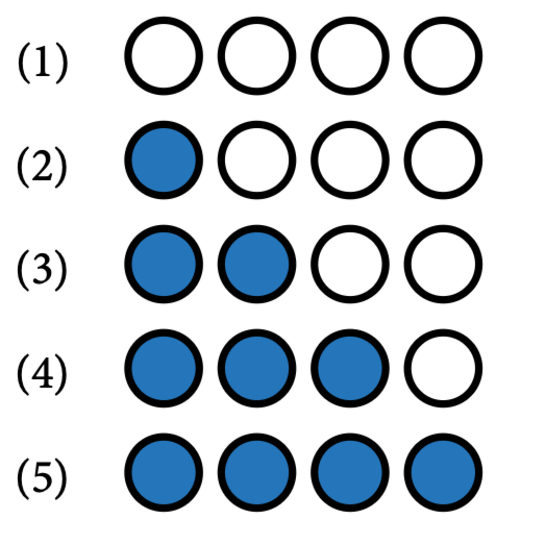
\includegraphics[height=75pt]{MarbleConjectures.pdf}
%%	\item We draw three marbles. \pause
%%	\item We observe: 
\includegraphics[width=35pt]{MarbleObservation.pdf}
%%    \end{itemize}
%%
%%%    \begin{figure}[!ht]
%%%    	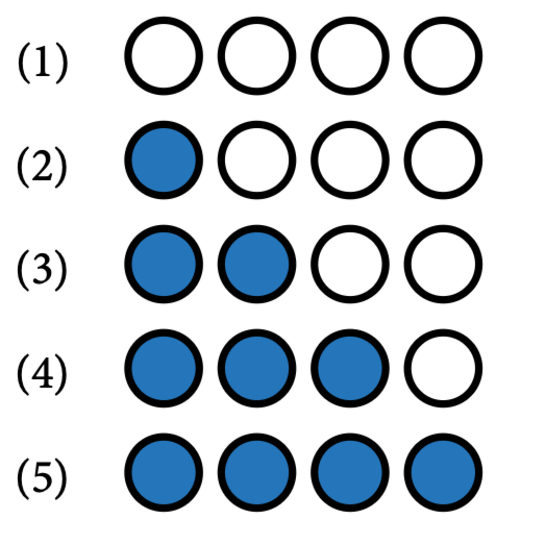
\includegraphics[height=75pt]{MarbleConjectures.pdf}
%%%    \end{figure}
%%\end{frame}
%
%\subsection{Are you a vampire?}
%
%\begin{frame}
%%    \begin{figure}[!ht]
%%    	
\includegraphics[width=100pt]{Vampire.jpg}
%%    \end{figure}
%    
%    \begin{itemize}
%    	\item There is a blood test that correctly detects vampirism 95\% of the time.
%	\begin{itemize}
%		\item \footnotesize A ``95\% success rate''
%	\end{itemize}
%    	\item One percent of the time it incorrectly diagnoses normal people.
%    	\item Vampires are only 0.1\% of the population.
%    	\item Say you test positive for vampirism:
%    	\begin{block}{}
%    		\centering
%    		What's the probability that you \textbf{really} are a vampire?
%    	\end{block}
%    \end{itemize}
%\end{frame}
%
%\begin{frame}
%We are told the following:
%	\begin{itemize}
%		\item $\mathbb{P}$ ( positive test result $\mid$ vampire ) = 0.95
%		\item $\mathbb{P}$ ( positive test result $\mid$ mortal ) = 0.01
%		\item $\mathbb{P}$ ( vampire ) = 0.001
%	\end{itemize}
%	We can now use Bayes' theorem to invert the probability to get $\mathbb{P}$( vampire $\mid$ positive ):
%	\begin{align*}
%		\mathbb{P} ( \text{vampire} \mid \text{positive} ) 	&= \frac{ \mathbb{P} ( \text{positive} \mid \text{vampire} ) \mathbb{P} ( \text{vampire} ) }{ \mathbb{P} ( \text{positive} ) }	\\
%		\mathbb{P} ( \text{positive} ) 					&= \mathbb{P} ( \text{positive} \mid \text{vampire} ) \mathbb{P} ( \text{vampire} ) + \\
%								&\qquad \mathbb{P} ( \text{positive} \mid \text{mortal} ) \left( 1 - \mathbb{P} ( \text{vampire} ) \right) \\
%												&= (0.95)(0.001) + (0.01)(0.999) = 0.0868
%	\end{align*}
%	Or an 8.7\% chance that the suspect is actually a vampire.
%\end{frame}
%
%\begin{frame}
%Not convinced? Ok let's try it a different way. Here is what we are given:
%	\begin{enumerate}
%		\item In a population of 100,000 people, 100 of them are vampires.
%		\item Of the 100 who are vampires, 95 of them will test positive for vampirism.
%		\item Of the 99,900 mortals, 999 will test positive for vampirism.
%	\end{enumerate}
%	So if we test all 100,000 people, what proportion of those who test positive for vampirism are actually vampires? 
%	\begin{itemize}
%		\item There are 95 + 999 = 1094 people who test positive. 
%		\item Of the 1094, 95 are really vampires. 
%		\item So: $\mathbb{P} ( \text{vampire} \mid \text{positive} ) = \frac{95}{1094} \approx 0.087$!
%	\end{itemize}
%	\begin{block}{Implication}
%		It's important to see here that a test that a ``95\% success rate'' ends up being right only $\approx$ 9\% of the time!
%	\end{block}
%\end{frame}
%
%\begin{frame}{Ten Coin Tosses}{Technical Details}
%	\begin{itemize}
%		\item The uninformed prior for the coin tosses are distributed uniformly between 0 and 1:
%		\begin{equation*}
%			p(H) \sim U(0,1)
%		\end{equation*}
%		\item The binomial likelihood is given by:
%		\begin{equation*}
%			\mathcal{L} \left( H \mid N, p \right) = \frac{N!}{H! (N - H)!} p^H (1 - p)^{N - H}
%		\end{equation*}
%		\item where:
%		\begin{itemize}
%			\item \footnotesize $N$ is the number of tosses, which in our final case was 10;
%			\item $H$ is the observed count of heads, which in our final case was 5;
%			\item $p$ is the probability of heads as defined above.
%			\begin{itemize}
%		 		\item The likelihood generates the data for all values of $p \in 0:1$.
%			\end{itemize}
%		\end{itemize}
%
%	\end{itemize}
%
%
%\end{frame}
%
%%\section{Appendix}
%%
%%\begin{frame}
%	
%
%%\section{Waterworld (An Example)}
%%
%%\begin{frame}
%%    \begin{figure}[!ht]
%%    	
\includegraphics[width=100pt]{Globe.jpg}
%%    \end{figure}
%%
%%\begin{itemize}
%%	\item Suppose you have a globe representing the plant Earth.
%%	\item You would like to estimate how much of the surface is covered in water.
%%	\item You do the following:
%%	\begin{itemize}
%%		\item You toss it in the air and catch it.
%%		\item Wherever your right index finger is, you record land (L) or water (W).
%%	\end{itemize}
%%\end{itemize}
%%
%%\end{frame}

\end{document}